%!TEX root = BCD.tex

%\section*{Results and Discussion}

%\subsection*{Determination of Kinetic and Thermodynamic Parameters}

%Simulation data and the resulting milestoning model were used to calculate 
%both \kon (figure \ref{fig:on_scatter}) and \koff (figure \ref{fig: off_scatter}).
%Values obtained from SEEKR with both GAFF\cite{Wang2004,Wang2006} and Q4MD\cite{Cezard2011} forcefields are compared to experimentally available values \cite{Fukahori2004,Fukahori2006,Nishikawa2002,Nishikawa2006,Rekharsky1998,Barros1998}
%as well as the calculated long timescale MD values from Tang et al\cite{Tang2017}.

%put actual values in table in SI?

%\subsubsection*{On Rates}

\par SEEKR calculations and the long timescale MD simulations struggle to 
reproduce both the values and rank ordering of the experimentally determined \kon's (Fig.~\ref{fig:on_scatter}).
\begin{figure}
	\begin{subfigure}{\linewidth}
	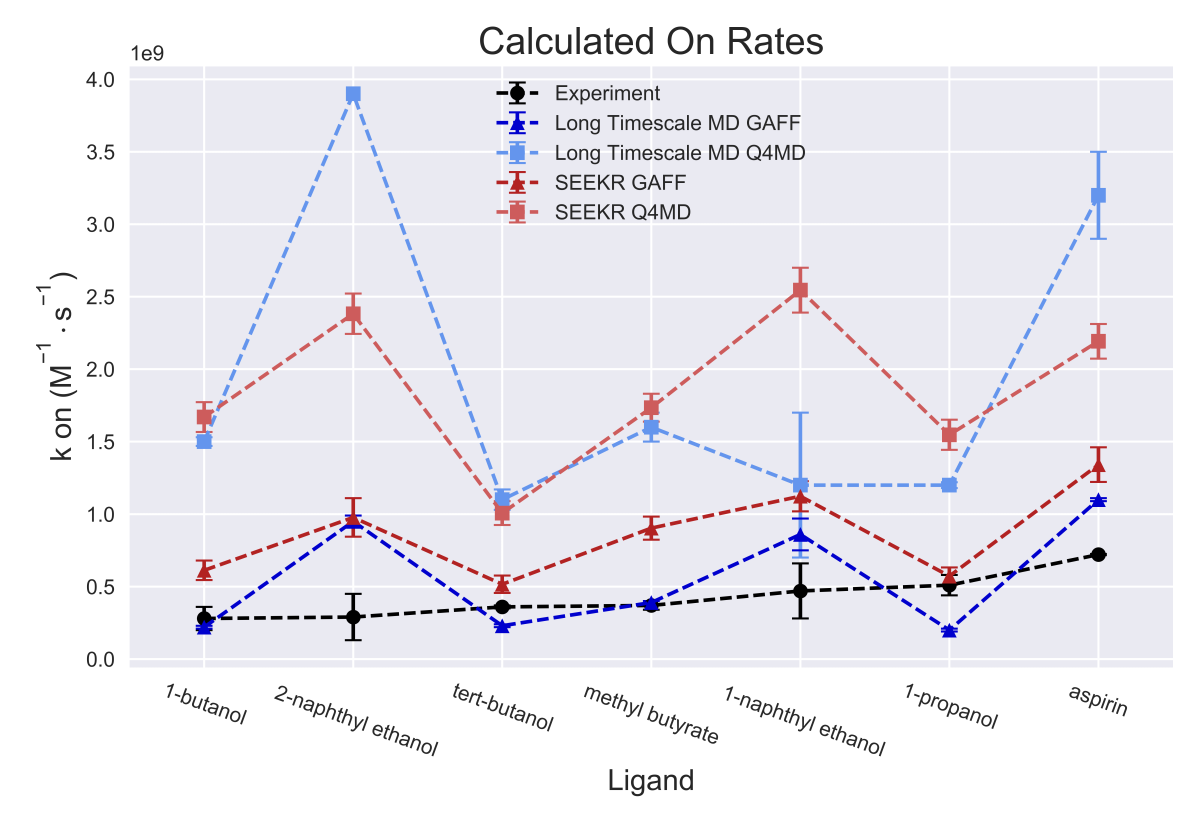
\includegraphics{images/on_scatter_resize.png}
	\caption{}
	\end{subfigure}

	\bigskip
	

	\begin{subfigure}{\linewidth}%<-- changed width
		%\centering
        %\renewcommand\tabularxcolumn[1]{m{#1}}% <-- added
        %\renewcommand\arraystretch{1.3}
        %\setlength\tabcolsep{2pt}% <-- added
    \begin{tabular}{
l  S[table-format = 2.3(3), separate-uncertainty] 
  S[table-format = 2.3(3), separate-uncertainty] 
 }%{\linewidth}%{*{4}{>{\centering\arraybackslash}X}}% <-- changed

\textbf{Method} & \textbf{Kendall} & \textbf{Spearman}  \\
\hline
      SEEKR GAFF      &    -0.20(31)           &    -0.29(40)            \\ 
      SEEKR Q4MD      &    0.14(29)           &    0.14(38)             \\ 
      Long Timescale MD GAFF      &    0.24(26)           &    0.25(29)                     \\ 
      Long Timescale MD Q4MD      &    0.00(28)           &    -0.05(37)                     \\ 
     

    \end{tabular}
        \caption{}
	\end{subfigure}
	\caption{a) Experimental and calculated on rates for SEEKR GAFF and Q4MD forcefields as well as long timescale MD with both forcefields. b) Calculated rank correlation coefficients. Errors are determined with a bootstrapping analysis. }
  \label{fig:on_scatter}
  \end{figure}
However, similar qualitative results are seen with the SEEKR calculations and 
long timescale MD calculations using the same forcefield.
%Chia-en directly from paper "GAFF-CD provided slightly more flexible β-CD, which produced more complicated H-bond
%networks between the free β-CD and water molecules in the first hydration shell, thereby resulting in slower kon and larger desolvation penalty"
On rates calculated using Q4MD are approximately one order of magnitude faster 
than experimental rates, while the GAFF forcefield produces rates closer to the 
experimental values, differing by approximately a factor of 3 or less.

\par Both methods fail to effectively order the ligands by increasing \kon, 
as demonstrated by low or negative Kendall and Spearman rank correlation coefficients.
As the values of all the experimental rates have limited variability (all within 
half an order of magnitude), the sensitivity of the methods as well as the errors 
associated with the calculations and experiments makes differentiation and 
ordering challenging. 
%Both simulation methods appear to show a stronger 
%dependence on the size and mass of the ligands than experiment, with both the 
%GAFF and Q4MD forcefields producing faster rates for larger compounds, a trend 
%not seen in the experimental rates.

%coment on uncharged small systems and how BD may struggle here?

 

%%!TEX root = BCD.tex

%%\documentclass[11pt,letterpaper]{article}

%%\usepackage{color}

%%\setlength{\textwidth}{17cm}
%%\setlength{\textheight}{20.5cm}
%%\setlength{\oddsidemargin}{-.1cm}
%%\setlength{\topmargin}{-2 cm}

%%\renewcommand{\baselinestretch}{1.0}

%%\newcommand{\hl}[1]{\textcolor{red}{#1}}
%\newcommand{\hl}[1]{\textbf{#1}}
%\providecommand{\e}[1]{\ensuremath{\times 10^{#1}}}

%%\begin{document}

\begin{table}

\centering
%\resizebox{\textwidth}{!}
{
\resizebox{\textwidth}{!}{\begin{tabular}{
l S[table-format = 2.3(3)e2, separate-uncertainty] |
l  S[table-format = 2.3(3)e2, separate-uncertainty] |
l S[table-format = 2.3(3)e2, separate-uncertainty]  |
l  S[table-format = 2.3(3)e2, separate-uncertainty] }

% \resizebox{\textwidth}{!}{\begin{tabular}{
% l S[table-format = 4.2(4)e8, separate-uncertainty, table-figures-uncertainty = 4.2] |
% l  S[table-format = 4.2e8, separate-uncertainty, table-figures-uncertainty = 4.2] |
% l S[table-format = 4.2e8, separate-uncertainty, table-figures-uncertainty = 4.2]  |
% l  S[table-format = 4.2e8, separate-uncertainty, table-figures-uncertainty = 4.2] |}

%\multicolumn{8}{c}{\kon rates}
\hline

 \multicolumn{2}{c}{\textbf{Experiment}} & \multicolumn{2}{c}{\textbf{SEEKR}} & \multicolumn{2}{c}{\textbf{Brute Force MD (GAFF)}} & \multicolumn{2}{c}{\textbf{Brute Force MD (Q4MD)}} \\ 
 \hline \hline


 \multirow{2}{*}{\textbf{ligand}} & \kon  & \multirow{2}{*}{\textbf{ligand}}	& \kon  & \multirow{2}{*}{\textbf{ligand}}	& \kon   & \multirow{2}{*}{\textbf{ligand}}	& \kon   \\
 & {(\si{\per\molar\per\second})} & & {(\si{\per\molar\per\second})} & & {(\si{\per\molar\per\second})} & & {(\si{\per\molar\per\second})} \\



 \hline

1-butanol & 2.8(8)e8 & \color{red}{1-propanol} & 6.53(50)e8 & \color{red}{1-propanol}	& 2.00(10)e8 & \color{red}{\textit{tert}-butanol} & 11.00(70)e8 \\ 

2-naphthylethanol &	2.90(190)e8	& \color{red}{\textit{tert}-butanol} 	& 7.25(47)e8	& \color{red}{1-butanol}		& 2.20(10)e8 & \color{red}{1-propanol} 	& 12.00(20)e8 \\

\textit{tert}-butanol &	3.60(10)e8 	& \color{red}{1-butanol} &	9.66(63)e8 	&\textit{tert}-butanol&	2.30(10)e8 	& \color{red}{1-naphthylethanol} &	12.00(500)e8 \\

methyl butyrate & 3.70(30)e8 &	methyl butyrate & 11.11(57)e8 &	methyl butyrate &	3.90(10)e8 & \color{red}{1-butanol} & 15.00(30)e8 \\

 1-naphthylethanol & 4.70(180)e8 & 1-naphthylethanol & 13.06(118)e8 & 1-naphthylethanol & 8.60(110)e8 &	\color{red}{methyl butyrate}& 16.00(100)e8 \\

1-propanol & 5.10(70)e8 & \color{red}{aspirin} &	16.29(74)e8 & \color{red}{2-naphthylethanol} & 9.50(40)e8 & \color{red}{aspirin} &	32.00(300)e8 \\


aspirin & 7.21(4)e8 & \color{red}{2-naphthylethanol} & 16.89(79)e8 &	aspirin & 11.00(10)e8 &	\color{red}{2-naphthylethanol} &	39.00e8 \\

\hline
&&\si{\tau} & 0.048(270) & \si{\tau} & 0.24(26) & \si{\tau} & 0.27(24) \\

\hline

\end{tabular}}
}
\caption{ Comparison of \kon values from experiment, SEEKR calculations, and brute force MD simulations with two different forcefields\cite{Tang2017}.
For each method, guest molecules are ranked in order of increasing rates.Ligands that are ordered incorrectly with respect to experiment are colored red. Kendall rank correlation coefficients (\si{\tau}) are also reported for each method.}
\label{table:kon-results}
\end{table}

%%\end{document}

 %add Q4MD and correct values if using

%\subsubsection*{Off Rates}



\par Unlike the experimental \kon's, \koff's for the seven guest 
molecules span multiple orders of magnitude, making them a better target for 
ranking the compounds with SEEKR.
%consider rewording this! 
Again, off rates calculated with SEEKR are in good agreement with the long 
timescale MD simulations using the same forcefield (Fig.~\ref{fig: off_scatter}). Rates calculated using the 
GAFF forcefield are consistently faster than experiment by approximately one 
order of magnitude. 
\begin{figure}
	\begin{subfigure}{\linewidth}
	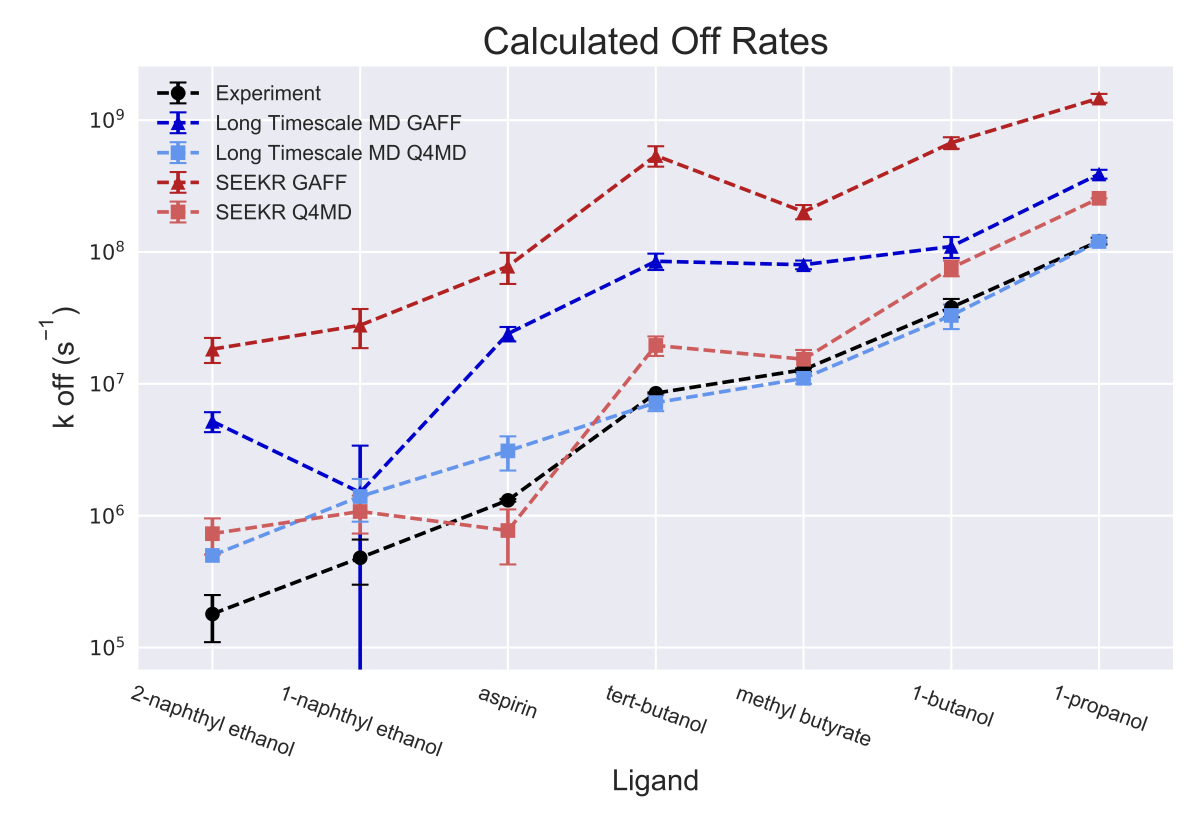
\includegraphics{images/off_scatter_resize.png}
	\caption{}
	\end{subfigure}

	\bigskip
	

	\begin{subfigure}{\linewidth}%<-- changed width
		%\centering
        %\renewcommand\tabularxcolumn[1]{m{#1}}% <-- added
        %\renewcommand\arraystretch{1.3}
        %\setlength\tabcolsep{2pt}% <-- added
    \begin{tabular}{
l  S[table-format = 2.3(3), separate-uncertainty] 
  S[table-format = 2.3(3), separate-uncertainty] 
 }%{\linewidth}%{*{4}{>{\centering\arraybackslash}X}}% <-- changed

\textbf{Method} & \textbf{Kendall} & \textbf{Spearman}  \\
\hline
      SEEKR GAFF      &    0.90(06)           &    0.96(04)            \\ 
      SEEKR Q4MD      &    0.81(09)           &    0.93(05)             \\ 
      Long Timescale MD GAFF      &    0.81(09)           &    0.93(04)                     \\ 
      Long Timescale MD Q4MD      &    01.00(05)           &    1.00(03)                     \\ 
     

    \end{tabular}
        \caption{}
	\end{subfigure}
	\caption{a) Experimental and calculated off rates for SEEKR GAFF and Q4MD forcefields as well as long timescale MD with both forcefields. b) Calculated rank correlation coefficients. Errors are determined with a bootstrapping analysis. }
	\label{fig: off_scatter}
\end{figure}
This trend is seen in both the long timescale MD and SEEKR, 
but is more pronounced in the SEEKR calculations. The Q4MD forcefield, however, 
more accurately reproduces the magnitude of the experimental values with both 
SEEKR and long timescale MD. SEEKR calculations with both Q4MD and GAFF 
forcefields were effective for ranking the compounds by increasing off rates, as evidenced by high rank correlation values.
%SEEKR with GAFF had a Kendall's $\tau = 0.90 \pm 0.06$ only mis-ordering the 
%tert-butanol and methyl butyrate ligands. The rank correlation coefficient for 
%SEEKR with Q4MD was slightly lower, $\tau = 0.81 \pm 0.09$ due to the additional 
%mis-ordering of the naphthyl ethanol ligands. 
The smaller magnitudes of the Q4MD 
values potentially contribute to this forcefield's difficulty to differentiate 
between compounds with similar rates, where the larger values associated with 
the GAFF forcefield allow for more variability in the rate value without changing 
the overall ordering. Both the GAFF and Q4MD forcefields successfully differentiate 
the three tighter binding compounds from the four weaker binding, with the tighter binding compounds 
all having slower off rates and a difference of one order of magnitude between 
the fastest tightly binding compound and the slowest weakly binding compound. This suggests that SEEKR 
could be useful for identifying and separating long residence time ligands from 
shorter residence time ligands and then further discriminating the compounds 
through ranking by \koff.


%%!TEX root = BCD.tex

%%\documentclass[11pt,letterpaper]{article}

%%\usepackage{color}

%%\setlength{\textwidth}{17cm}
%%\setlength{\textheight}{20.5cm}
%%\setlength{\oddsidemargin}{-.1cm}
%%\setlength{\topmargin}{-2 cm}

%%\renewcommand{\baselinestretch}{1.0}

%%\newcommand{\hl}[1]{\textcolor{red}{#1}}
%\newcommand{\hl}[1]{\textbf{#1}}
%\providecommand{\e}[1]{\ensuremath{\times 10^{#1}}}

%%\begin{document}

\begin{table}

\centering
%\resizebox{\textwidth}{!}
{
%\resizebox{\textwidth}{!}{\begin{tabular}{l S@{\pm} S l S @{\,\( \pm \)\,} S l S @{\,\( \pm \)\,} S l S@{\,\( \pm \)\,} S}
\resizebox{\textwidth}{!}{\begin{tabular}{
l S[table-format = 4.2(3)e2, separate-uncertainty] |
l  S[table-format = 4.2(4)e2, separate-uncertainty] |
l S[table-format = 4.2(4)e2, separate-uncertainty]  |
l  S[table-format = 2.3(1)e2, separate-uncertainty] } 

%\multicolumn{8}{c}{\kon rates}
\hline
 \multicolumn{2}{c}{\textbf{Experiment}} & \multicolumn{2}{c}{\textbf{SEEKR}} & \multicolumn{2}{c}{\textbf{Brute Force MD (GAFF)}} & \multicolumn{2}{c}{\textbf{Brute Force MD (Q4MD)}} \\ 
 \hline \hline

 \multirow{2}{*}{\textbf{ligand}} & \koff  & \multirow{2}{*}{\textbf{ligand}}	& \koff  & \multirow{2}{*}{\textbf{ligand}}	& \koff   & \multirow{2}{*}{\textbf{ligand}}	& \koff   \\
 & {(\si{\per\second})} & & {(\si{\per\second})} & & {(\si{\per\second})} & & {(\si{\per\second})} \\



 \hline

2-naphthylethanol &	1.8(7)e6 &	\color{red}{1-naphthylethanol} & 	0.87(34)e6 &	 \color{red}{1-naphthylethanol}	& 1.50(190)e6 & 	2-naphthylethanol	& 0.5  \\
 1-naphthylethanol & 0.48(18)e6 & 	\color{red}{2-naphthylethanol} &	3.43(72)e6	& \color{red}{2-naphthylethanol}	& 5.20(90)e6	 & 1-naphthylethanol& 	1.4(5)e6 \\
aspirin & 	1.31(3)e6 &	aspirin & 	49.31(710)e6 & 	aspirin &	24.00(300)e6 & 	aspirin & 	3.1(9)e6 \\
\textit{tert}-butanol	& 8.50(10)e6 &	\color{red}{methyl butyrate} &	158.35(1550)e6 &	\color{red}{methyl butyrate} &	80.00(600)e6	& \textit{tert}-butanol &	7.2(10)e6 \\
methyl butyrate &	12.80(30)e6 & 	\color{red}{\textit{tert}-butanol} &	258.74(2793)e6 &	\color{red}{\textit{tert}-butanol} &	85.00(1200)e6 &	methyl butyrate &	11(1)e6 \\
1-butanol &	38.00(600)e6 &	1-butanol &	512.16(3745)e6 &	1-butanol &	110.00(2000)e6 &	1-butanol &	33(7)e6 \\
1-propanol &	121.00(700)e6 &	1-propanol &	1495.42(7686)e6 &	1-propanol &	390.00(3000)e6 &	1-propanol&	120(2)e6 \\
\hline

&&\si{\tau} & 0.81(5) & \si{\tau} & 0.81(9) & \si{\tau} & 1.00(4) \\

\hline

\end{tabular}}
}
\caption{ Comparison of \koff values from experiment, SEEKR calculations, and brute force MD simulations with two different forcefields\cite{Tang2017}.
For each method, guest molecules are ranked in order of increasing rates. Ligands that are ordered incorrectly with respect to experiment are colored red. Kendall rank correlation coefficients (\si{\tau}) are also reported for each method.}
\label{table:koff-results}
\end{table}

%%\end{document} %add Q4MD and correct values if using

%\subsubsection*{Binding Free Energy}
\par An additional benefit of kinetics calculations with SEEKR is that binding 
free energies can also be obtained from the same simulations (Fig.~\ref{fig:dg_scatter}). 
\begin{figure}
	\begin{subfigure}{\linewidth}
	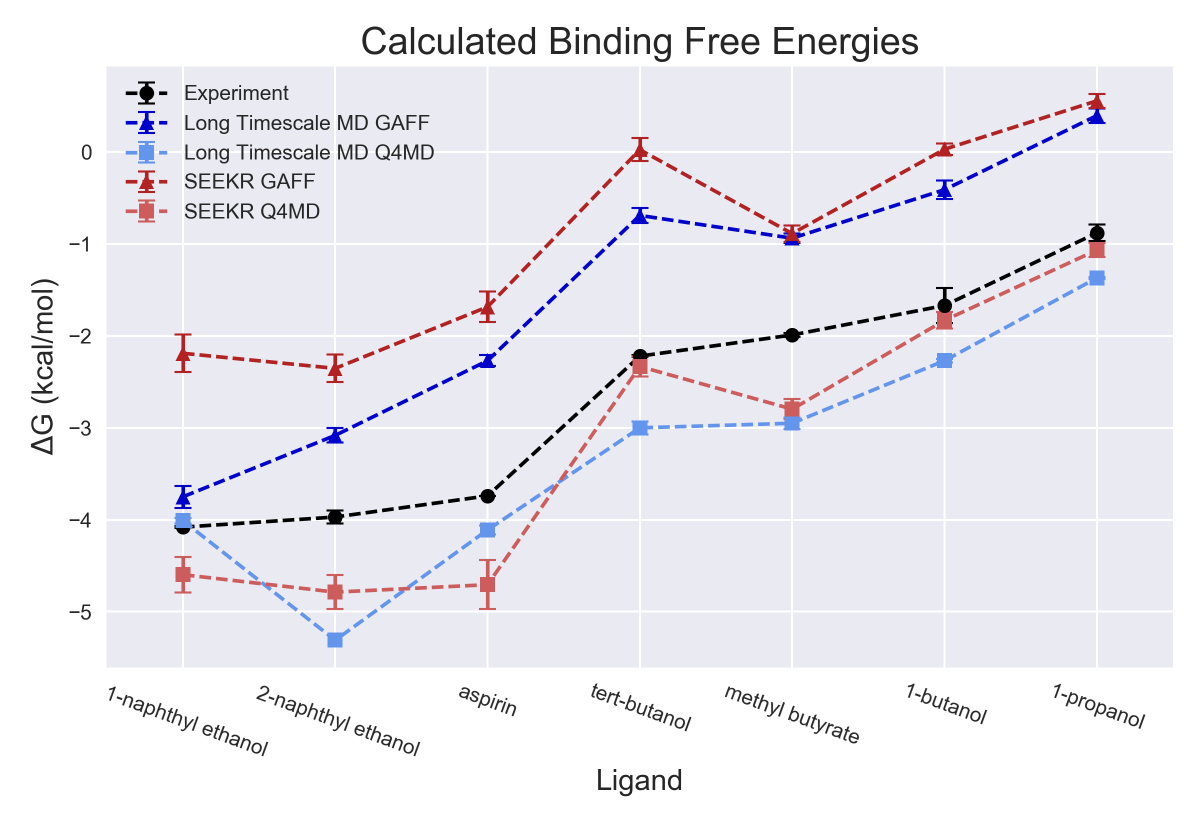
\includegraphics{images/dg_scatter_resize.png}
	\caption{}
	\end{subfigure}
	\bigskip
	\begin{subfigure}{\linewidth}%<-- changed width
		\centering
        %\renewcommand\tabularxcolumn[1]{m{#1}}% <-- added
        %\renewcommand\arraystretch{1.3}
        %\setlength\tabcolsep{2pt}% <-- added
	    \begin{tabular}{
	    	l  S[table-format = 2.3(3), separate-uncertainty] 
	  		S[table-format = 2.3(3), separate-uncertainty] 
	 	}%{\linewidth}%{*{4}{>{\centering\arraybackslash}X}}% <-- changed

			\textbf{Method} & \textbf{Kendall} & \textbf{Spearman}  \\
			\hline
	        SEEKR GAFF      &    0.88(08)           &    0.96(05)            \\ 
	        SEEKR Q4MD      &    0.73(10)           &    0.89(06)             \\ 
	        Long Timescale MD GAFF      &    0.90(07)           &    0.96(04)                     \\ 
	        Long Timescale MD Q4MD      &    0.87(11)           &    0.94(06)                     \\ 
	     

	    \end{tabular}
        \caption{}
	\end{subfigure}
	\caption{a) Experimental and calculated binding free energies for SEEKR GAFF and Q4MD forcefields as well as long timescale MD with both forcefields. b) Calculated rank correlation coefficients. Errors are determined with a bootstrapping analysis. }
	
	\label{fig:dg_scatter}
\end{figure}
Binding free energies calculated using the rate constants %$\Delta G= -RTln(k_{\textrm{on}}/k_{\textrm{off}})$, 
are most heavily influenced by the \koff for these ligands, as this value is more variable, where 
the \kon's for all ligands are more similar. Therefore, similar trends are observed 
for the calculated binding free energies as were observed for the off rates.
Binding free energies can also be calculated using the stationary probabilities 
for each milestone, rather than the rate constants, and produce similar results.
The GAFF forcefield consistently underestimates the binding free energies in both 
SEEKR and the long timescale MD, resulting from the consistent underestimation 
of the magnitudes of the \koff's. The magnitudes of the binding free 
energies calculated using Q4MD are in much better agreement with the experimental 
values, differing by 1 kcal or less. SEEKR with both Q4MD and GAFF successfully 
differentiates the three known tighter binding compounds from the four weaker binding compounds.
%Experimentally, there is a difference of 1.52 kcal/mol between the two groups.
%The GAFF calculation underestimates this difference, calculating a difference of 
%$0.79 \pm 0.19$ kcal/mol between the aspirin and methyl butyrate ligands while SEEKR 
%with Q4MD slightly overestimates the difference, calculating a difference of 
%$1.8 \pm 0.11$  kcal/mol between 1-naphthyl ethanol and methyl butyrate. Again 
%this suggests that SEEKR is a useful tool for differentiating tight binders 
%from weaker binders. 
SEEKR can also further discriminate ligands 
by its effective ranking %of ligands 
by binding free energies, demonstrated by high rank correlation values.

%producing Kendal 
%rank correlation values of $0.88 \pm 0.08$ for GAFF and $0.73 \pm 0.1$ for Q4MD.



%%!TEX root = BCD.tex

%%\documentclass[11pt,letterpaper]{article}

%%\usepackage{color}

%%\setlength{\textwidth}{17cm}
%%\setlength{\textheight}{20.5cm}
%%\setlength{\oddsidemargin}{-.1cm}
%%\setlength{\topmargin}{-2 cm}

%%\renewcommand{\baselinestretch}{1.0}

%%\newcommand{\hl}[1]{\textcolor{red}{#1}}
%\newcommand{\hl}[1]{\textbf{#1}}
%\providecommand{\e}[1]{\ensuremath{\times 10^{#1}}}

%%\begin{document}

\begin{table}

\centering
%\resizebox{\textwidth}{!}
{
\resizebox{\textwidth}{!}{\begin{tabular}{
l S[table-format = 1.2(2), separate-uncertainty] |
l  S[table-format = 1.2(2), separate-uncertainty] |
l S[table-format = 1.2(2), separate-uncertainty]  |
l  S[table-format = 1.2(2), separate-uncertainty] }

% \resizebox{\textwidth}{!}{\begin{tabular}{
% l S[table-format = 4.2(4)e8, separate-uncertainty, table-figures-uncertainty = 4.2] |
% l  S[table-format = 4.2e8, separate-uncertainty, table-figures-uncertainty = 4.2] |
% l S[table-format = 4.2e8, separate-uncertainty, table-figures-uncertainty = 4.2]  |
% l  S[table-format = 4.2e8, separate-uncertainty, table-figures-uncertainty = 4.2] |}

%\multicolumn{8}{c}{\kon rates}
\hline

 \multicolumn{2}{c}{\textbf{Experiment}} & \multicolumn{2}{c}{\textbf{SEEKR}} & \multicolumn{2}{c}{\textbf{Brute Force MD (GAFF)}} & \multicolumn{2}{c}{\textbf{Brute Force MD (Q4MD)}} \\ 
 \hline \hline


 \multirow{2}{*}{\textbf{ligand}} & $\Delta G$  & \multirow{2}{*}{\textbf{ligand}}	& $\Delta G$  & \multirow{2}{*}{\textbf{ligand}}	& $\Delta G$   & \multirow{2}{*}{\textbf{ligand}}	& $\Delta G$   \\
 & {(\si{\kcal\per\mol})} & & {(\si{\kcal\per\mol})} & & {(\si{\kcal\per\mol})} & & {(\si{\kcal\per\mol})} \\



 \hline

1-naphthylethanol & -4.08(1) & 1-naphthylethanol & -4.33(24) & 1-naphthylethanol	& -3.75(12) & \color{red}{2-naphthylethanol} & -5.31 \\ 

2-naphthylethanol &	-3.97(7)	& 2-naphthylethanol 	& -3.67(13)	& 2-naphthylethanol		& -3.08(8) & \color{red}{aspirin} 	& -4.11(5) \\

aspirin &	-3.74(00) 	& aspirin &	-2.07(9) 	& aspirin &	-2.27(6) 	& \color{red}{1-naphthylethanol} &	-4.01(03) \\

\textit{tert}-butanol & -2.22(1) &	\color{red}{methyl butyrate} & -1.15(7) &	\color{red}{methyl butyrate} &	-0.94(5) & \textit{tert}-butanol & -3.00(7) \\

 methyl butyrate & -1.99(2) & \color{red}{\textit{tert}-butanol} & -0.61(7) & \color{red}{\textit{tert}-butanol} & -0.69(8) &	methyl butyrate & -2.95(6) \\

1-butanol & -1.67(19) & 1-butanol &	-0.38(6) & 1-butanol & -0.41(10) & 1-butanol &	-2.27(2) \\


1-propanol & -0.88(9) & 1-propanol & 0.49(6) &	1-propanol & 0.40(8) &	1-propanol &	-1.37(1) \\

\hline
&&\si{\tau} & 0.90(7) & \si{\tau} & 0.90(7) & \si{\tau} & 0.87(10) \\

\hline

\end{tabular}}
}
\caption{ Comparison of \kon values from experiment, SEEKR calculations, and brute force MD simulations with two different forcefields\cite{Tang2017}.
For each method, guest molecules are ranked in order of increasing rates.Ligands that are ordered incorrectly with respect to experiment are colored red. Kendall rank correlation coefficients (\si{\tau}) are also reported for each method.}
\label{table:dG-results}
\end{table}

%%\end{document}


\par A key aspect of future development of the SEEKR software is the systematic 
development of methodological best-practices as well as the elucidation of the 
sensitivity of calculated kinetic parameters to various SEEKR input conditions.

%\subsubsection*{Sampling}
While it is possible to determine the kinetics for small systems like 
$\beta$-cyclodextrin using conventional long timescale MD simulations, increasing 
system size soon makes this inefficient or even impossible. 
%The advantage of the 
%SEEKR approach is twofold; 1) reducing the  simulation time required to obtain 
%accurate kinetics and 2) reducing the overall time required for calculations by 
%employing a highly parallel approach. The current bottleneck for SEEKR calculations 
%is obtaining the equilibrium distribution, which still requires relatively long MD simulations on the order of hundreds of nanoseconds per milestone. It is therefore of great interest to reduce the amount 
%of simulation necessary for achieving converged rate values.
The convergence of \kon and \koff were assessed by calculating the rate 
constants as a function of the reversal trajectory number at increasing intervals 
of 50 reversal numbers (with 10 trajectories initiated for each reversal number).
The reversal number is a direct measure of the equilibrium simulation length, as 
reversals are initiated from evenly spaced configurations of the equilibrium distribution.
In general, both the on and off rates appear converged in less than the maximum 
number of reversals available. Approximately half the total reversals 
(4000 of 8000) were sufficient for obtaining reasonably converged rate constants. 
This suggests that the total simulation cost to obtain a similar result could be 
as little as 2 ${\mu}s$ per ligand, rather than 3.8 ${\mu}s$.

%\begin{figure}
\begin{subfigure}{0.3\linewidth}
	\centering
	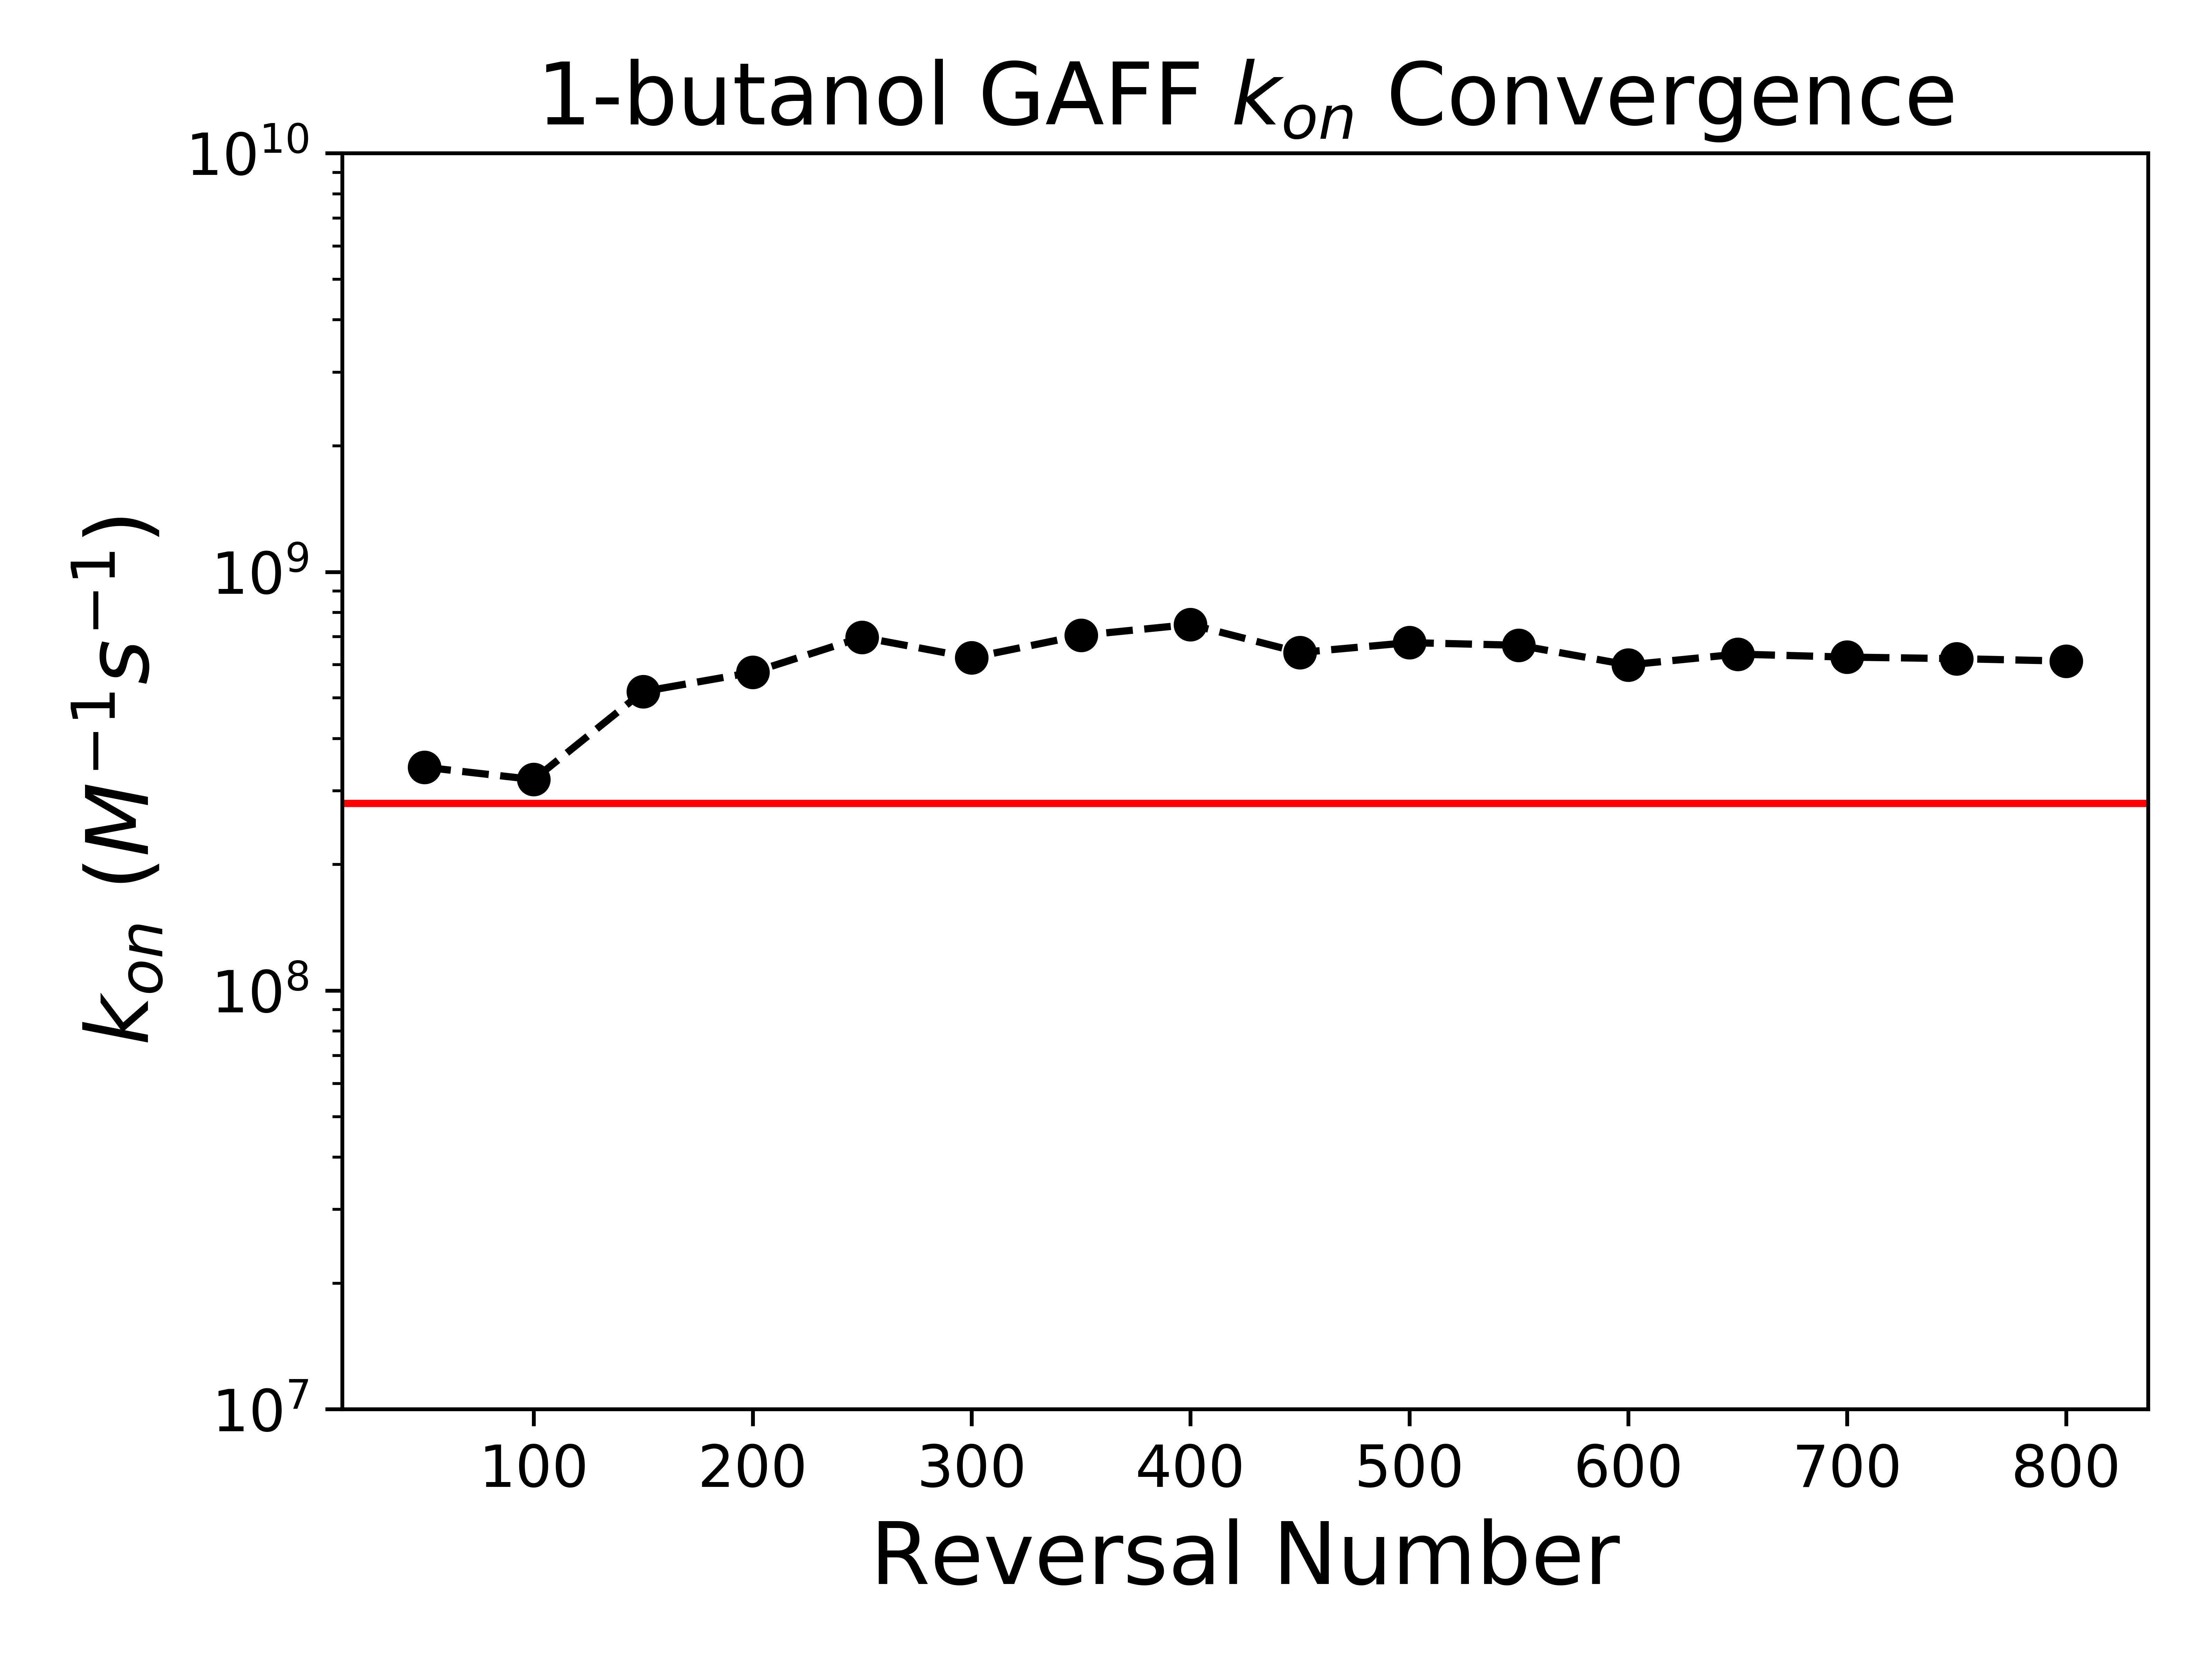
\includegraphics[width=\linewidth]{high_res_images/gaff_rate_conv_images/1-butanol_gaff_on_conv.png}
	\end{subfigure}%
\begin{subfigure}{0.3\linewidth}
		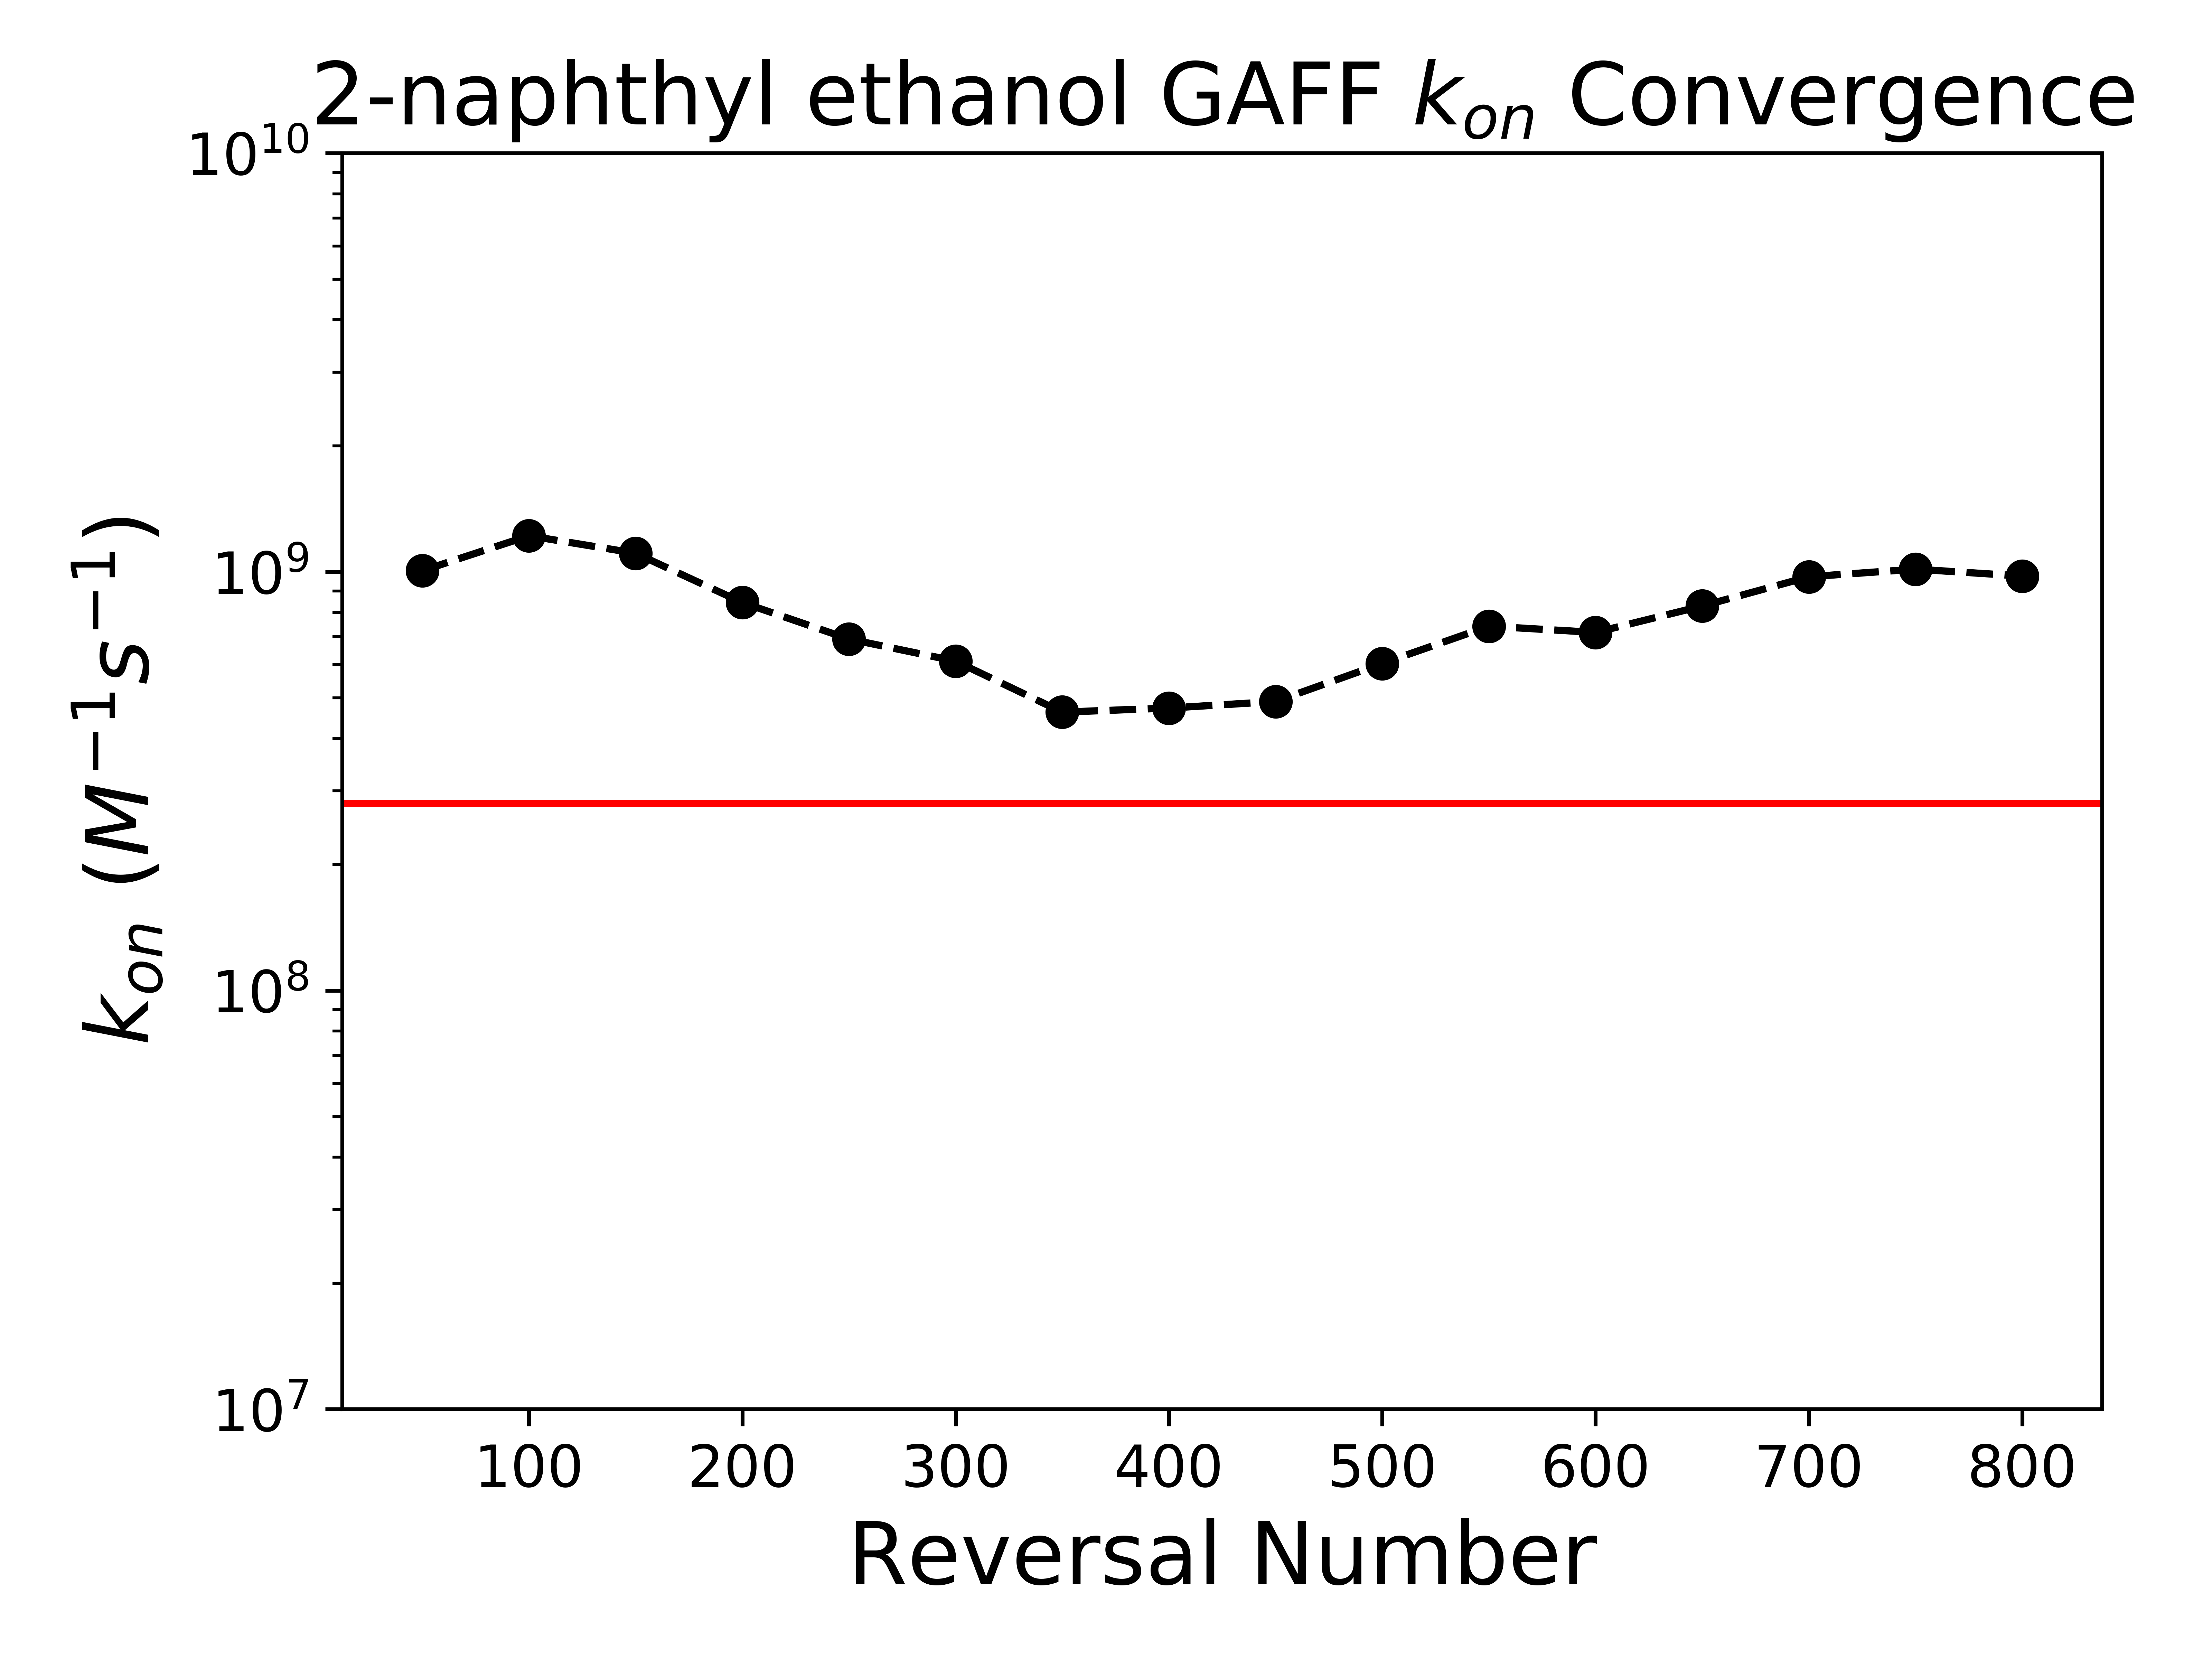
\includegraphics[width=\linewidth]{high_res_images/gaff_rate_conv_images/2-naphthylethanol_gaff_on_conv.png}
\end{subfigure}%
	\begin{subfigure}{0.3\linewidth}
		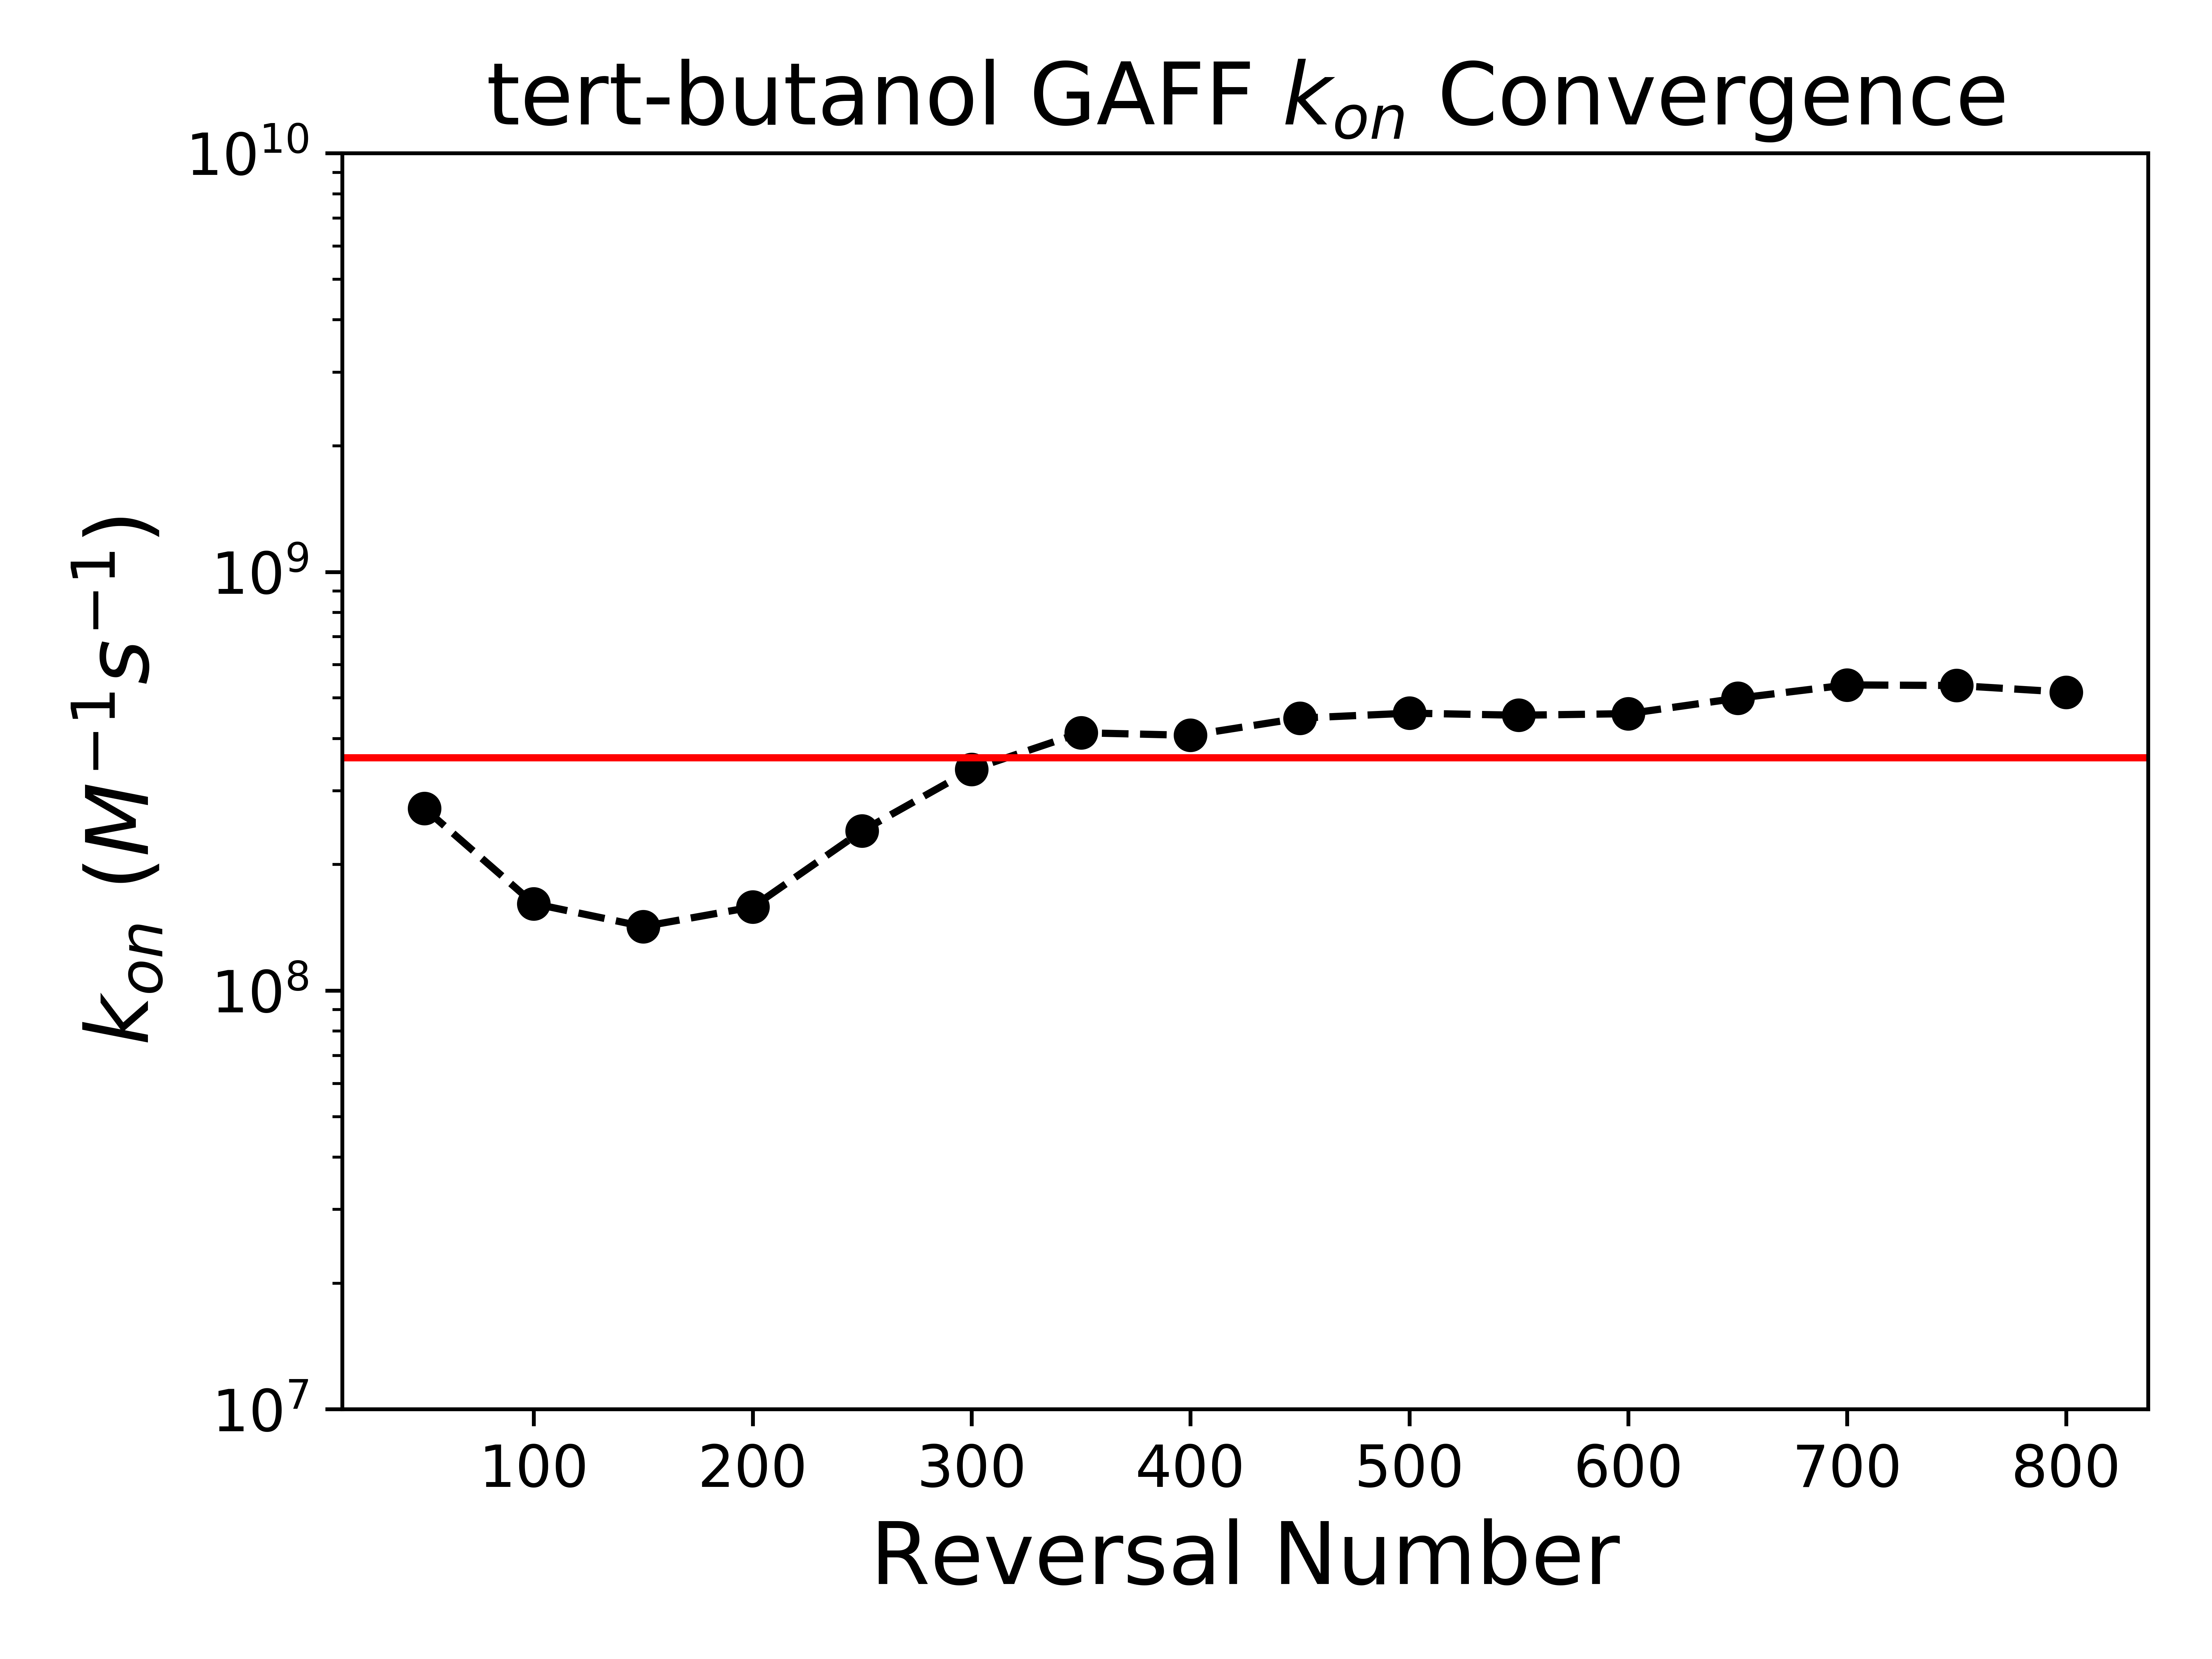
\includegraphics[width=\linewidth]{high_res_images/gaff_rate_conv_images/tert-butanol_gaff_on_conv.png}
	\end{subfigure}
	\begin{subfigure}{0.3\linewidth}
		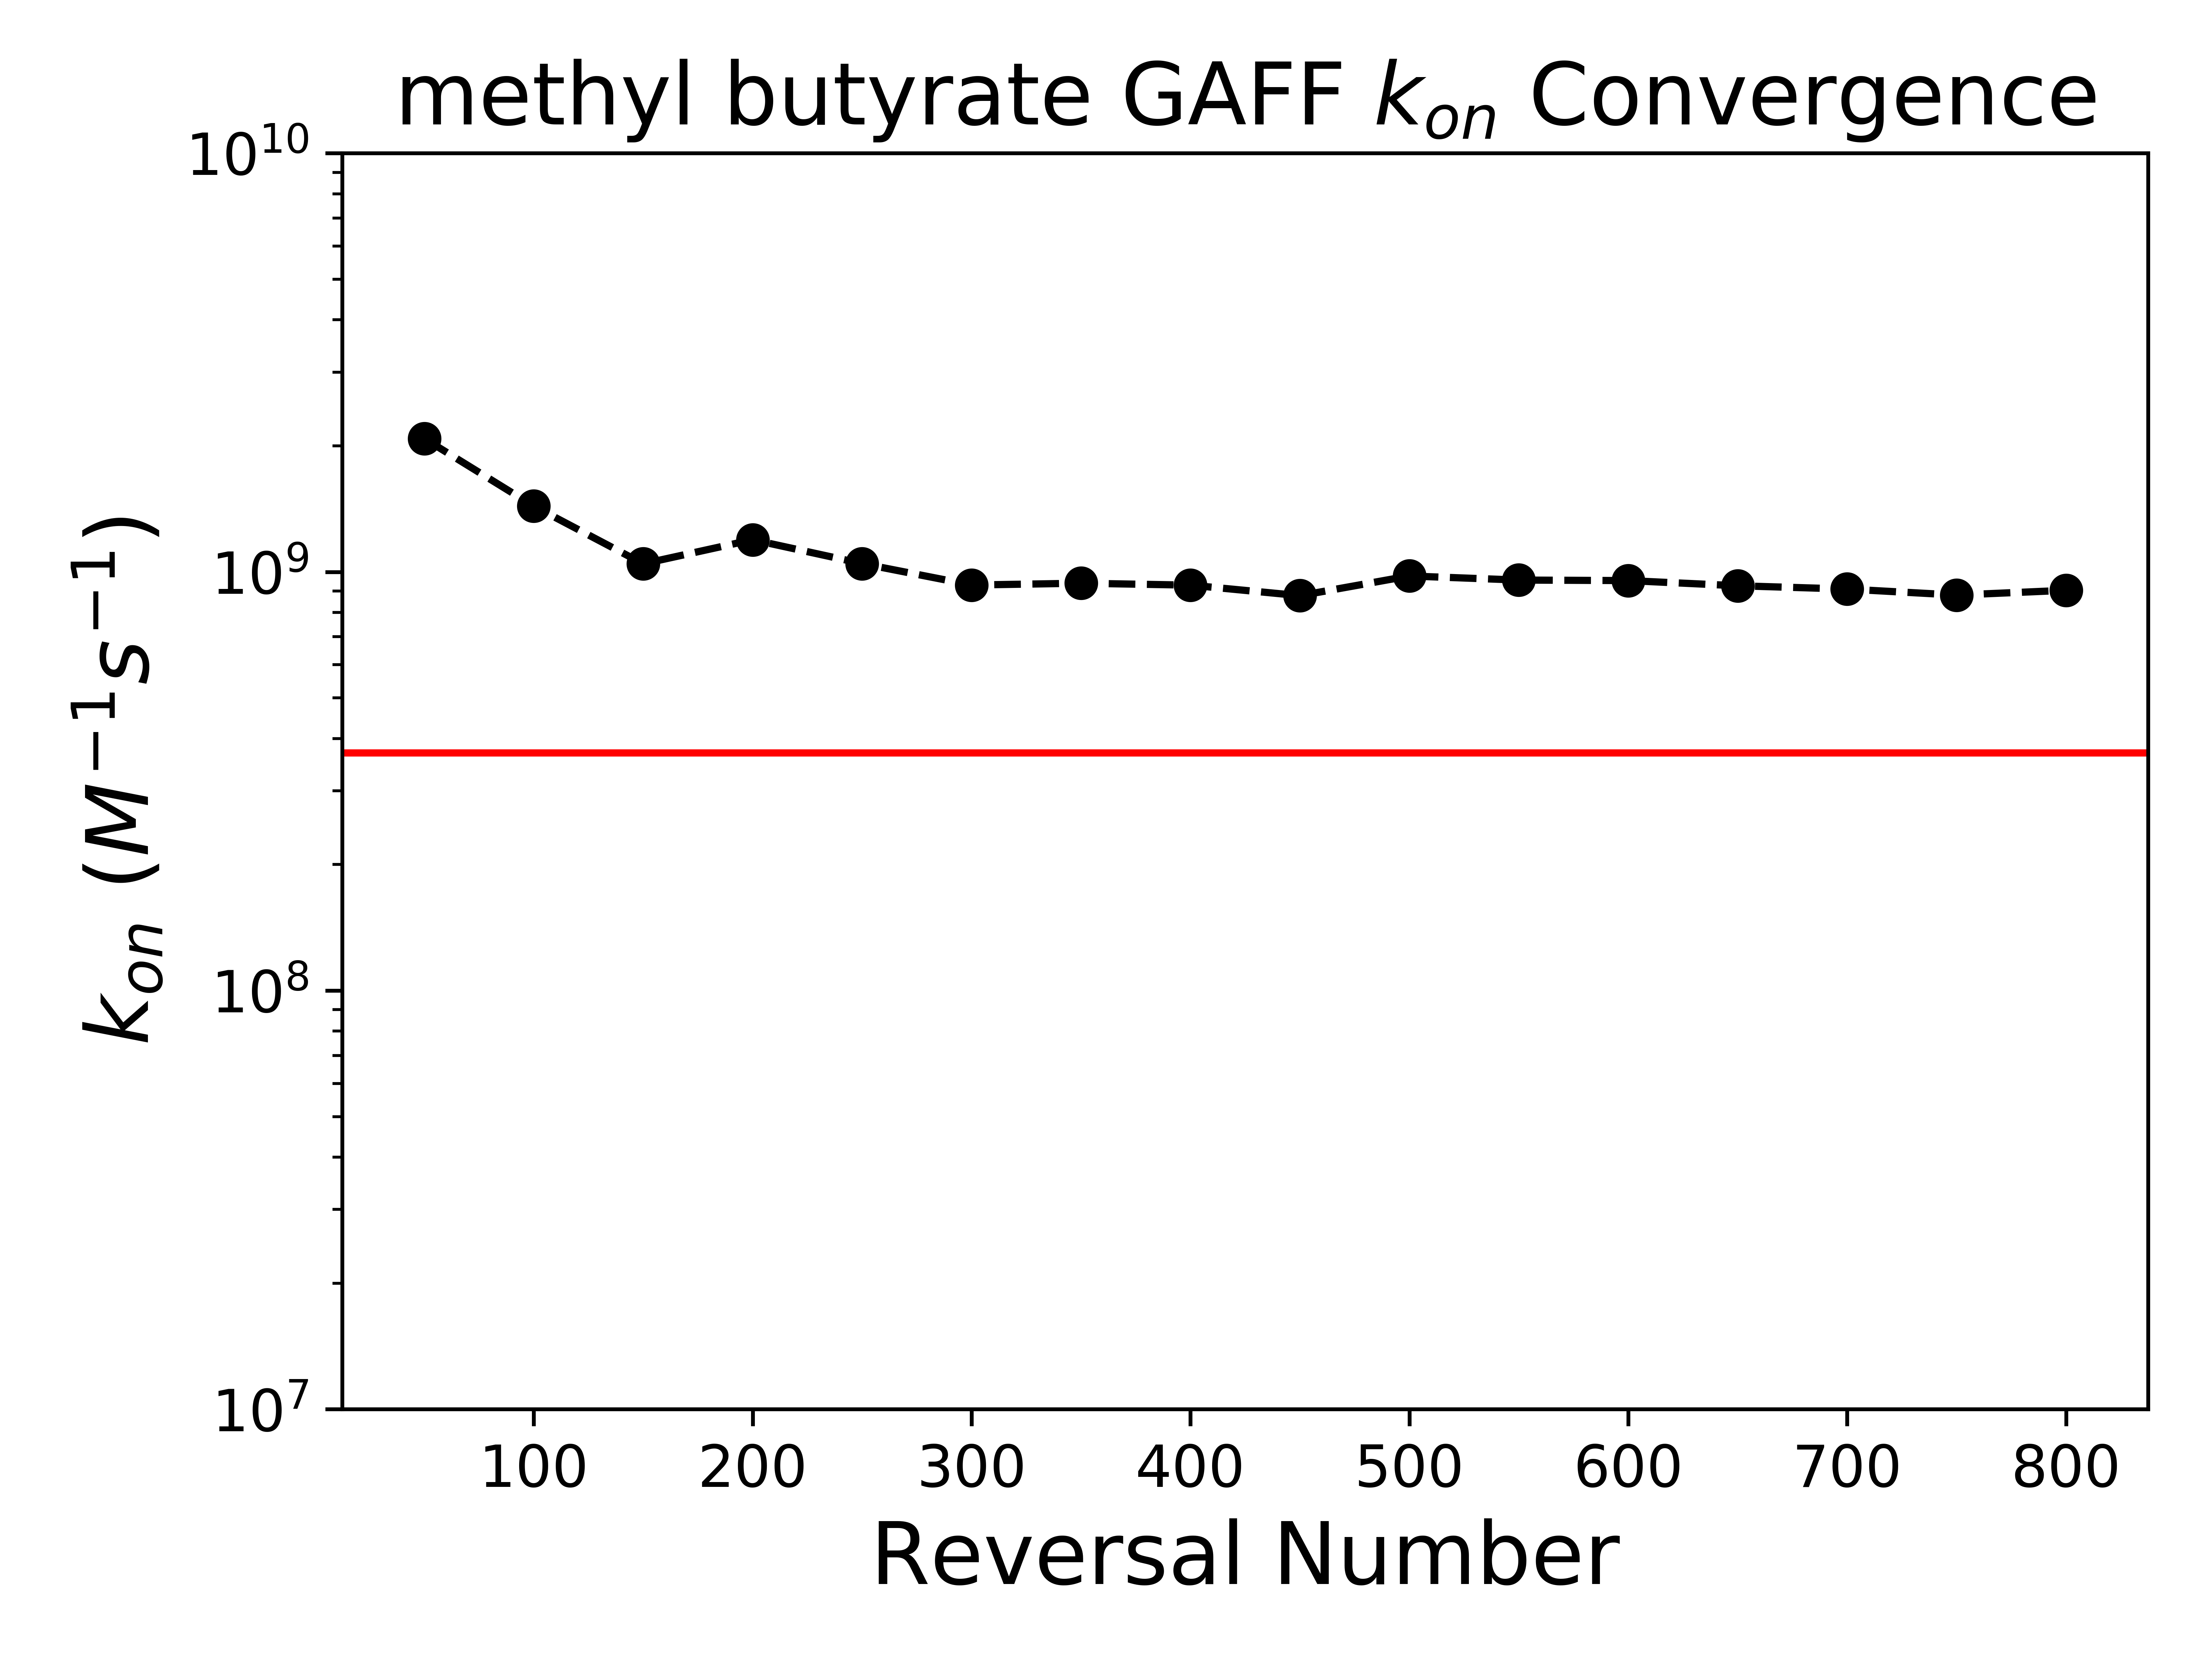
\includegraphics[width=\linewidth]{high_res_images/gaff_rate_conv_images/methylbutyrate_gaff_on_conv.png}
	\end{subfigure}
	\begin{subfigure}{0.3\linewidth}
		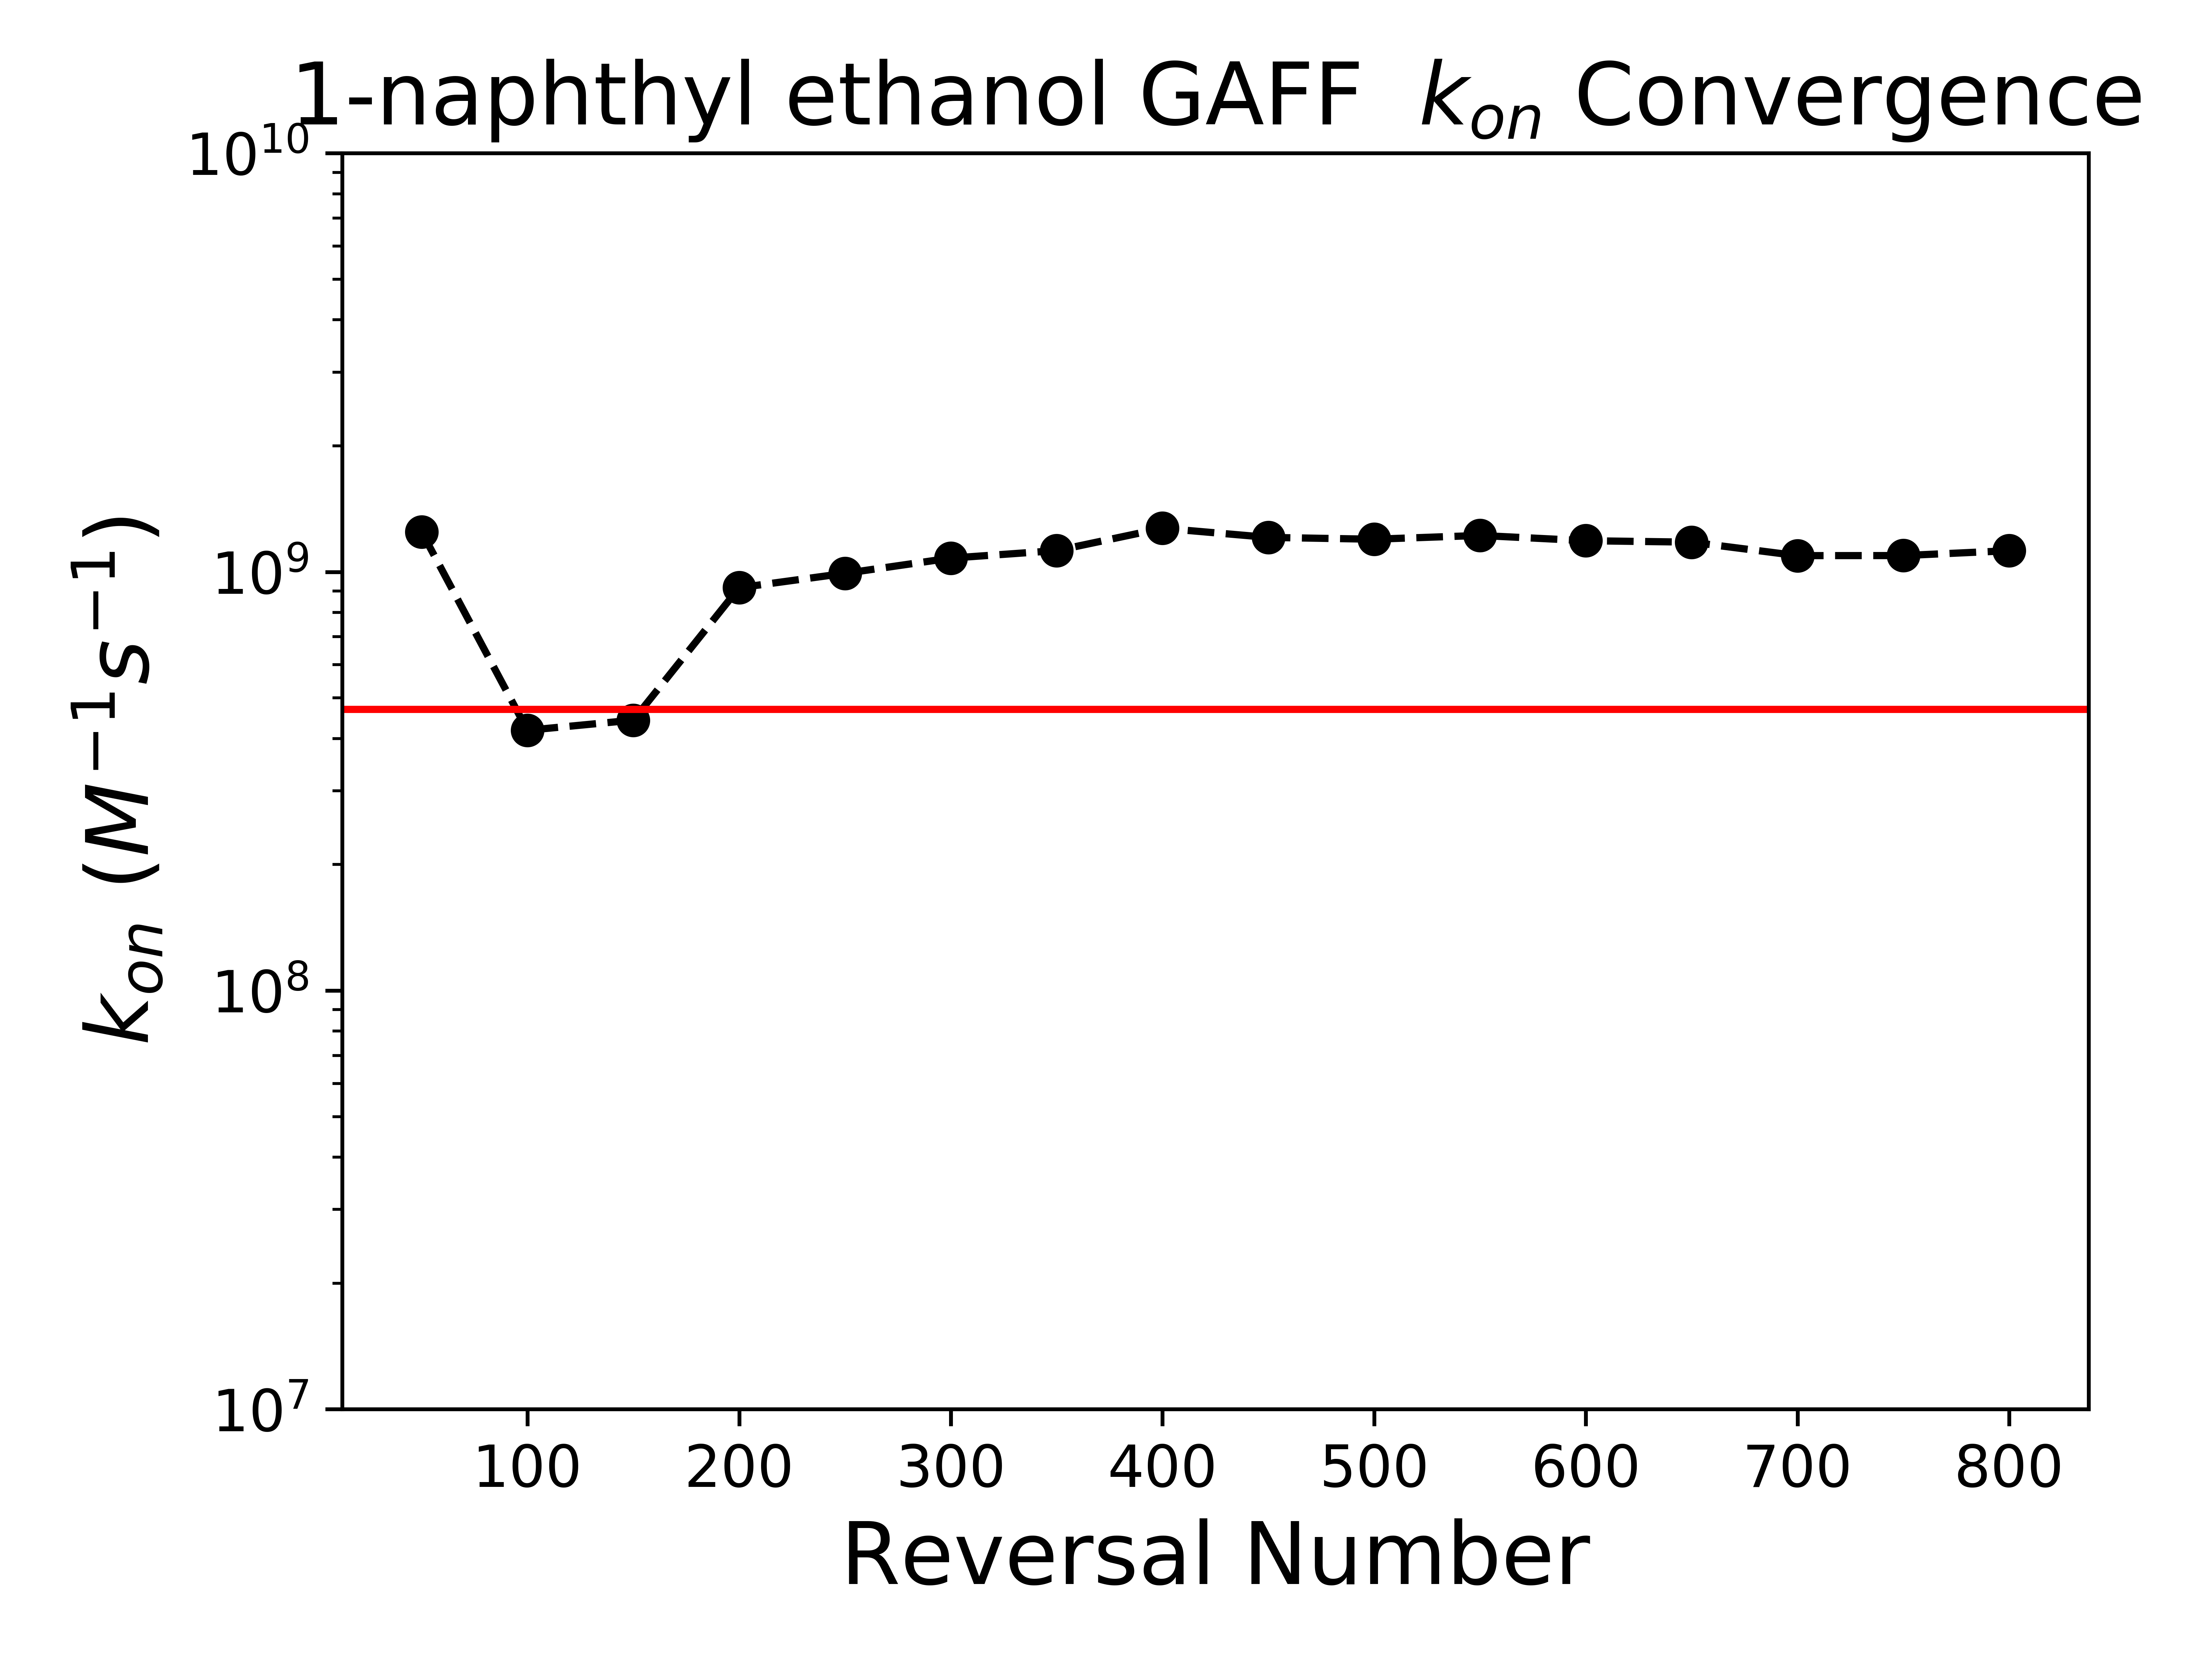
\includegraphics[width=\linewidth]{high_res_images/gaff_rate_conv_images/1-naphthylethanol_gaff_on_conv.png}
	\end{subfigure}
	\begin{subfigure}{0.3\linewidth}
		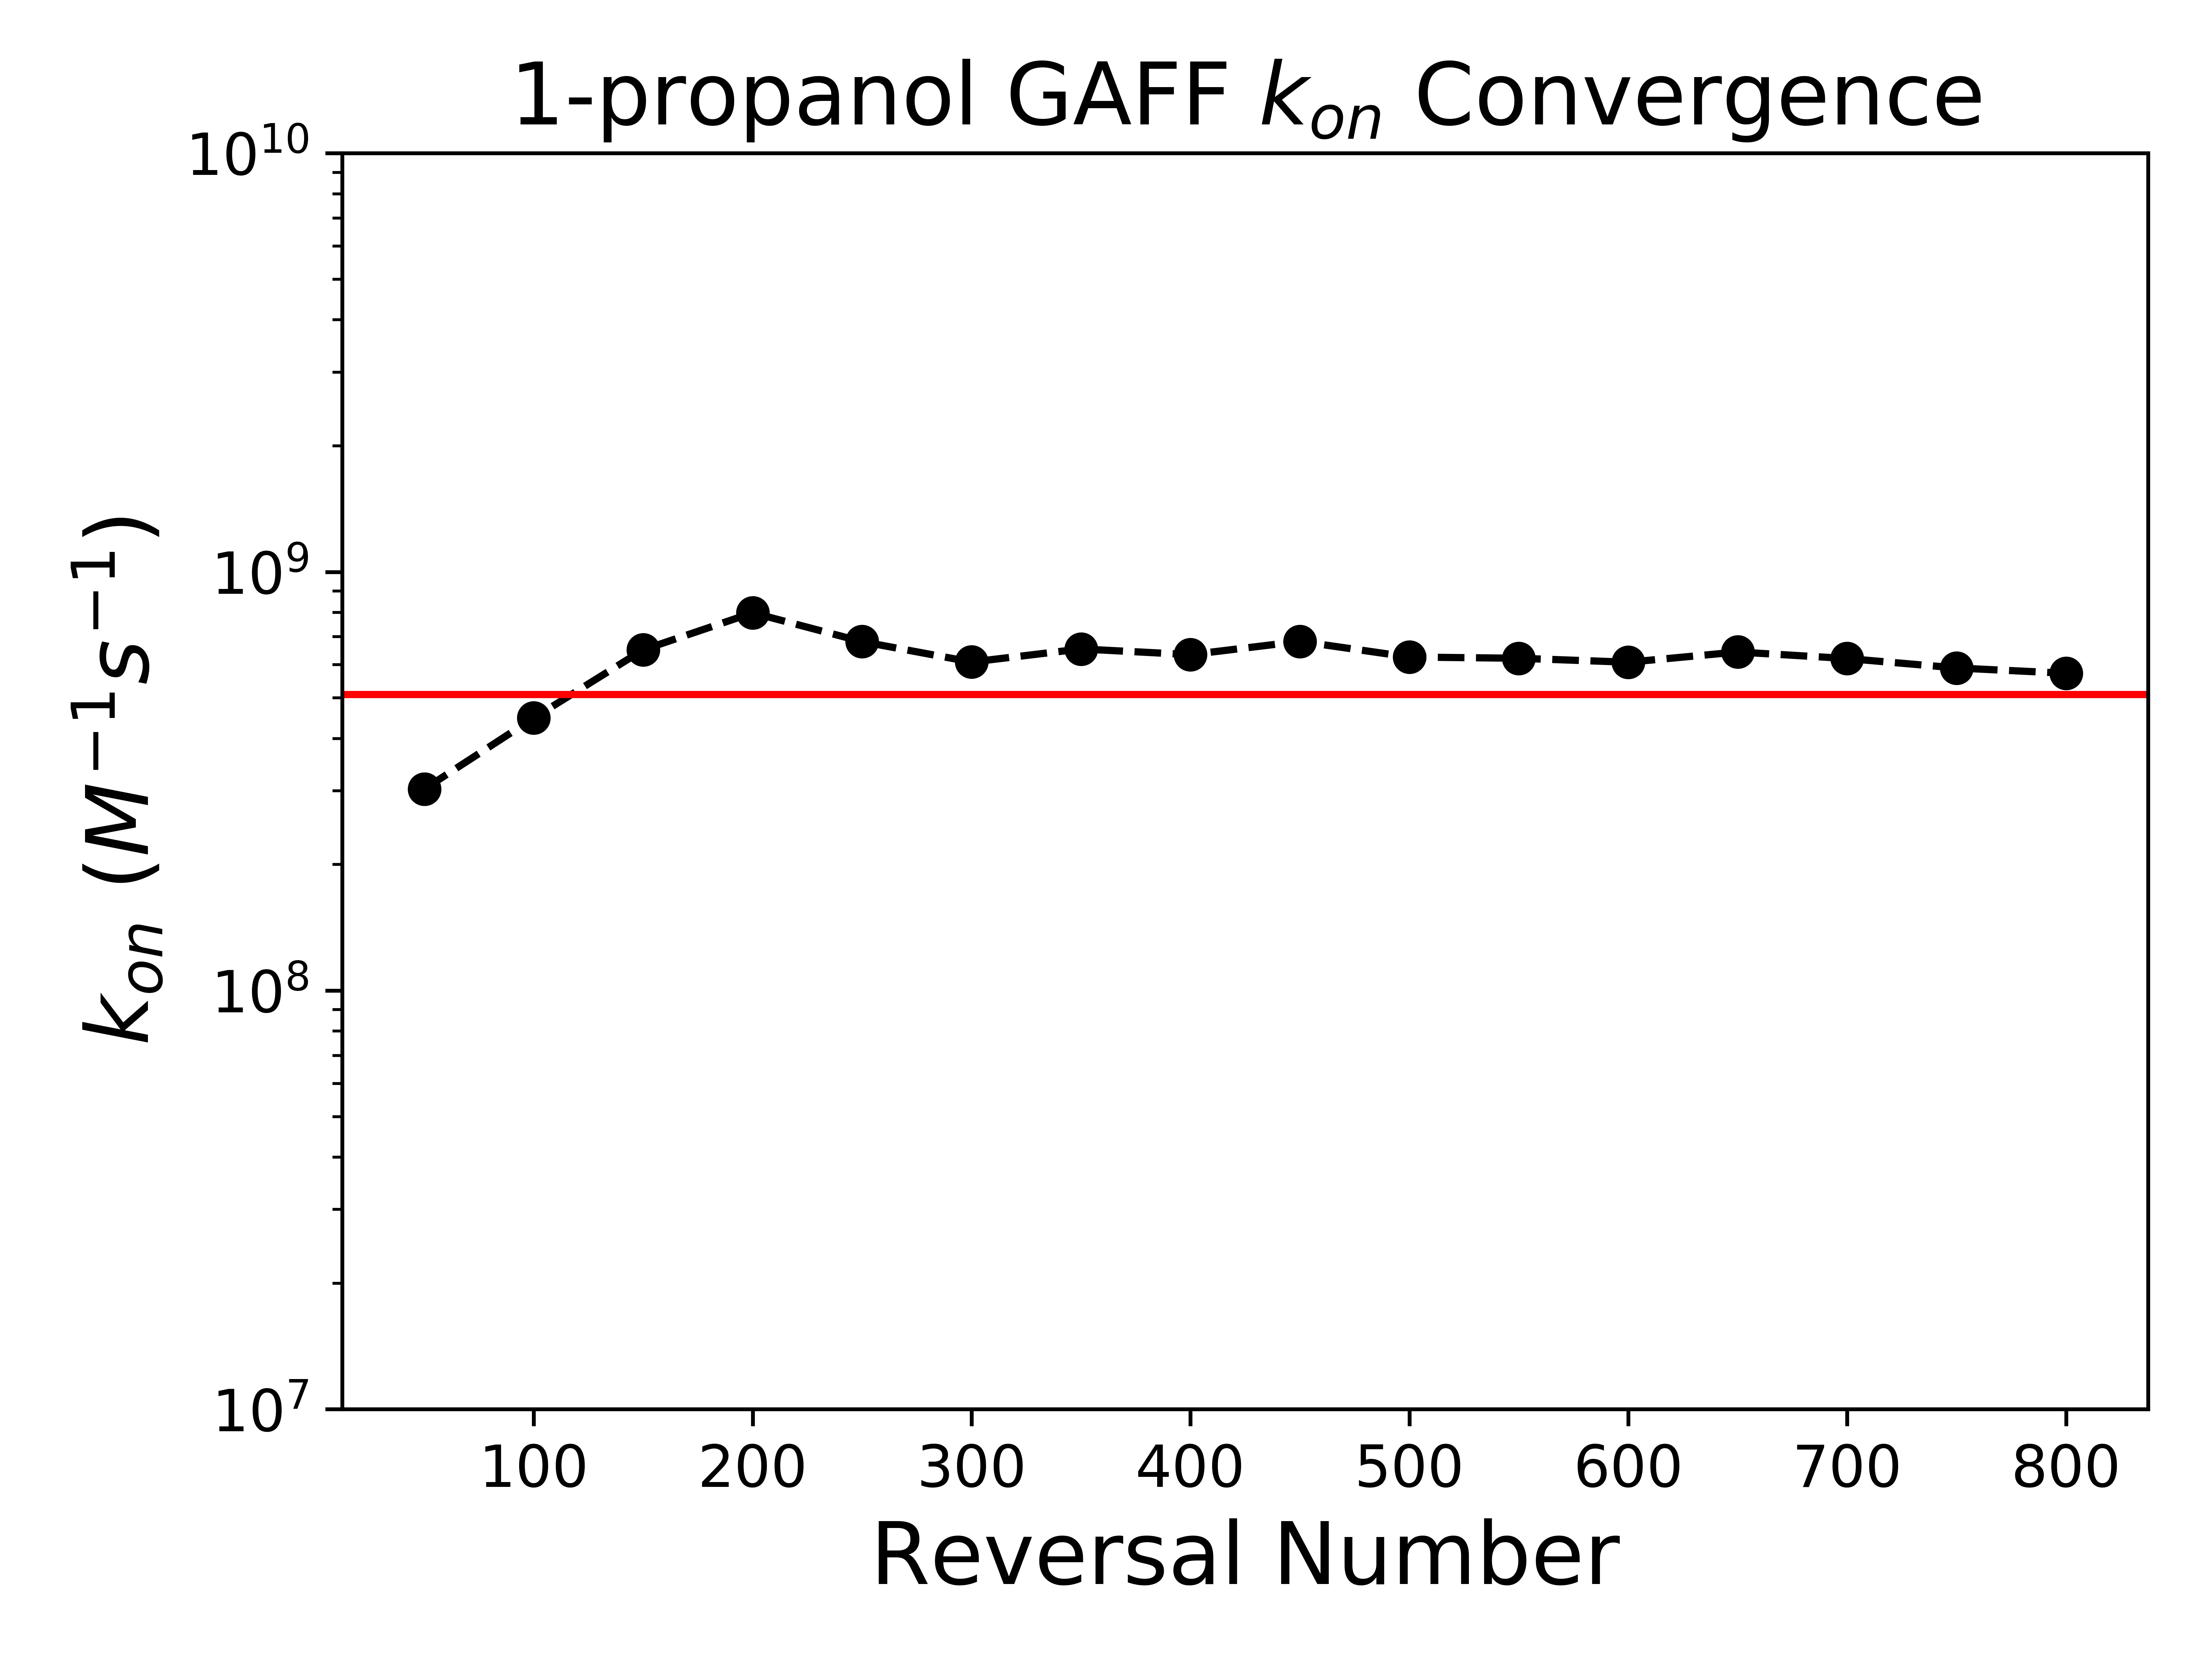
\includegraphics[width=\linewidth]{high_res_images/gaff_rate_conv_images/1-propanol_gaff_on_conv.png}
	\end{subfigure}
	\begin{subfigure}{0.3\linewidth}
		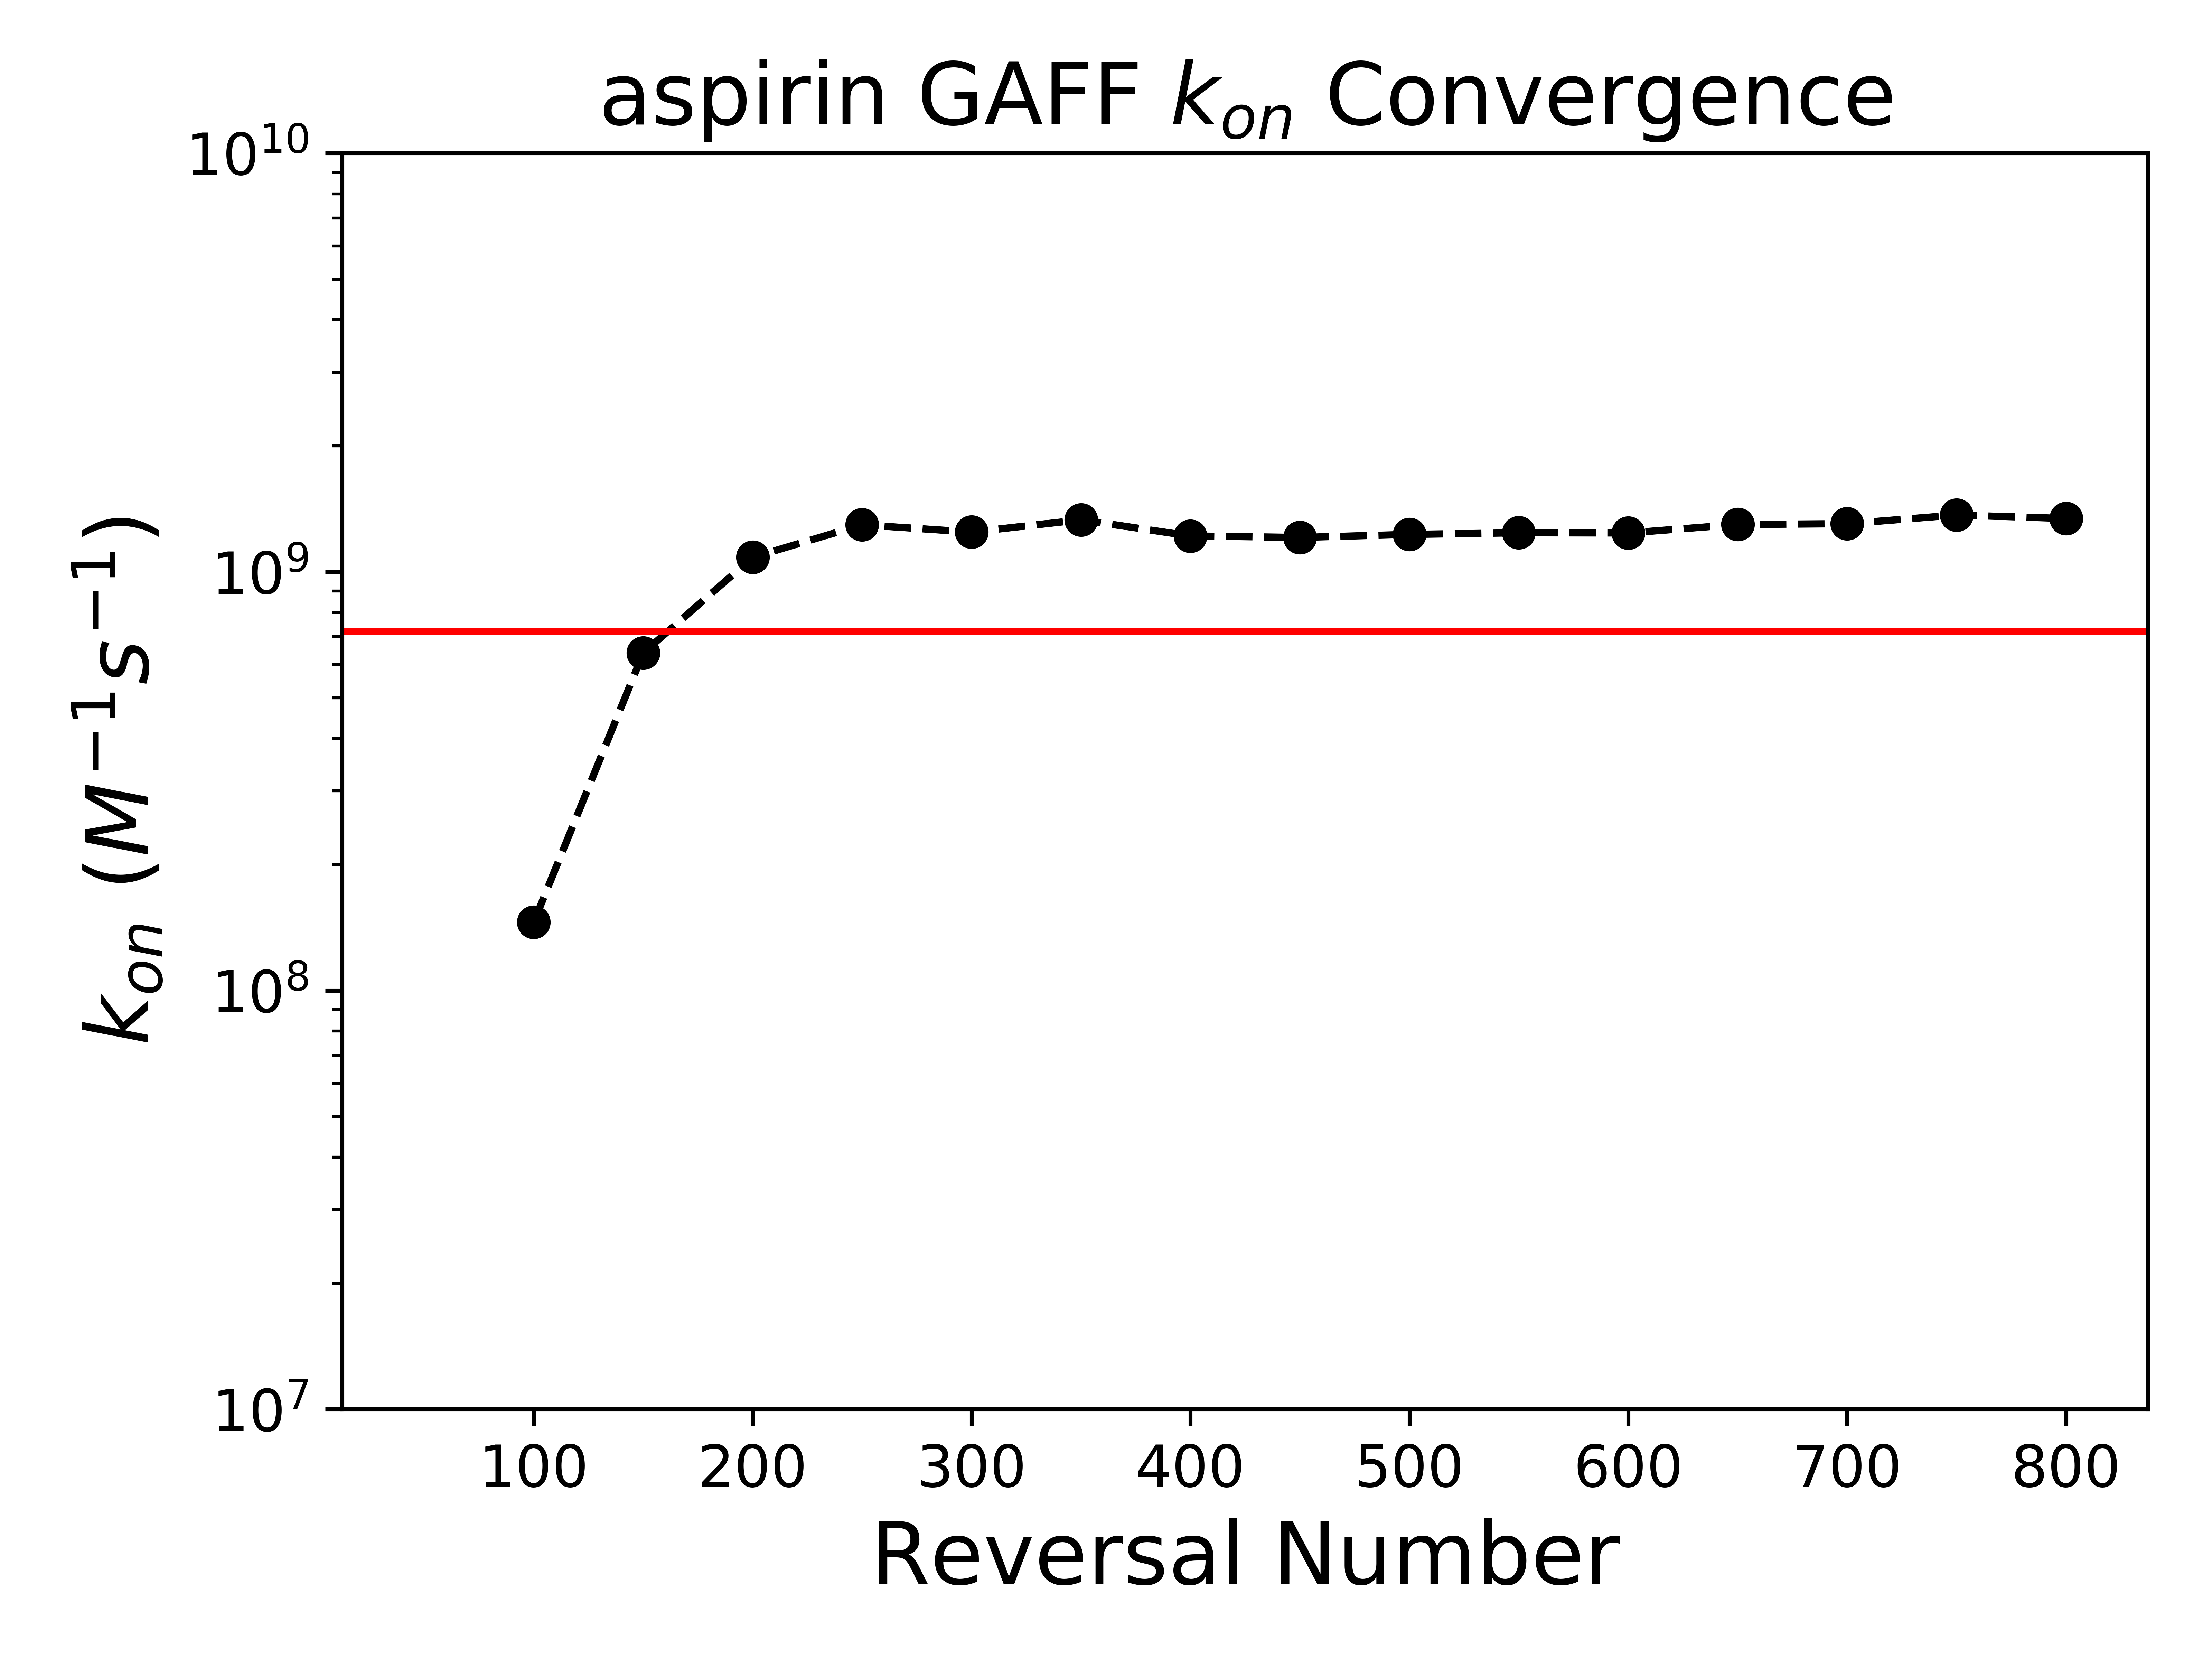
\includegraphics[width=\linewidth]{high_res_images/gaff_rate_conv_images/aspirin_gaff_on_conv.png}
	\end{subfigure}
	\caption{Convergence of on rates as a function of the number of reversals included using the GAFF forcefield}
\end{figure}
%\begin{figure}
\centering
	\begin{subfigure}{0.3\linewidth}
	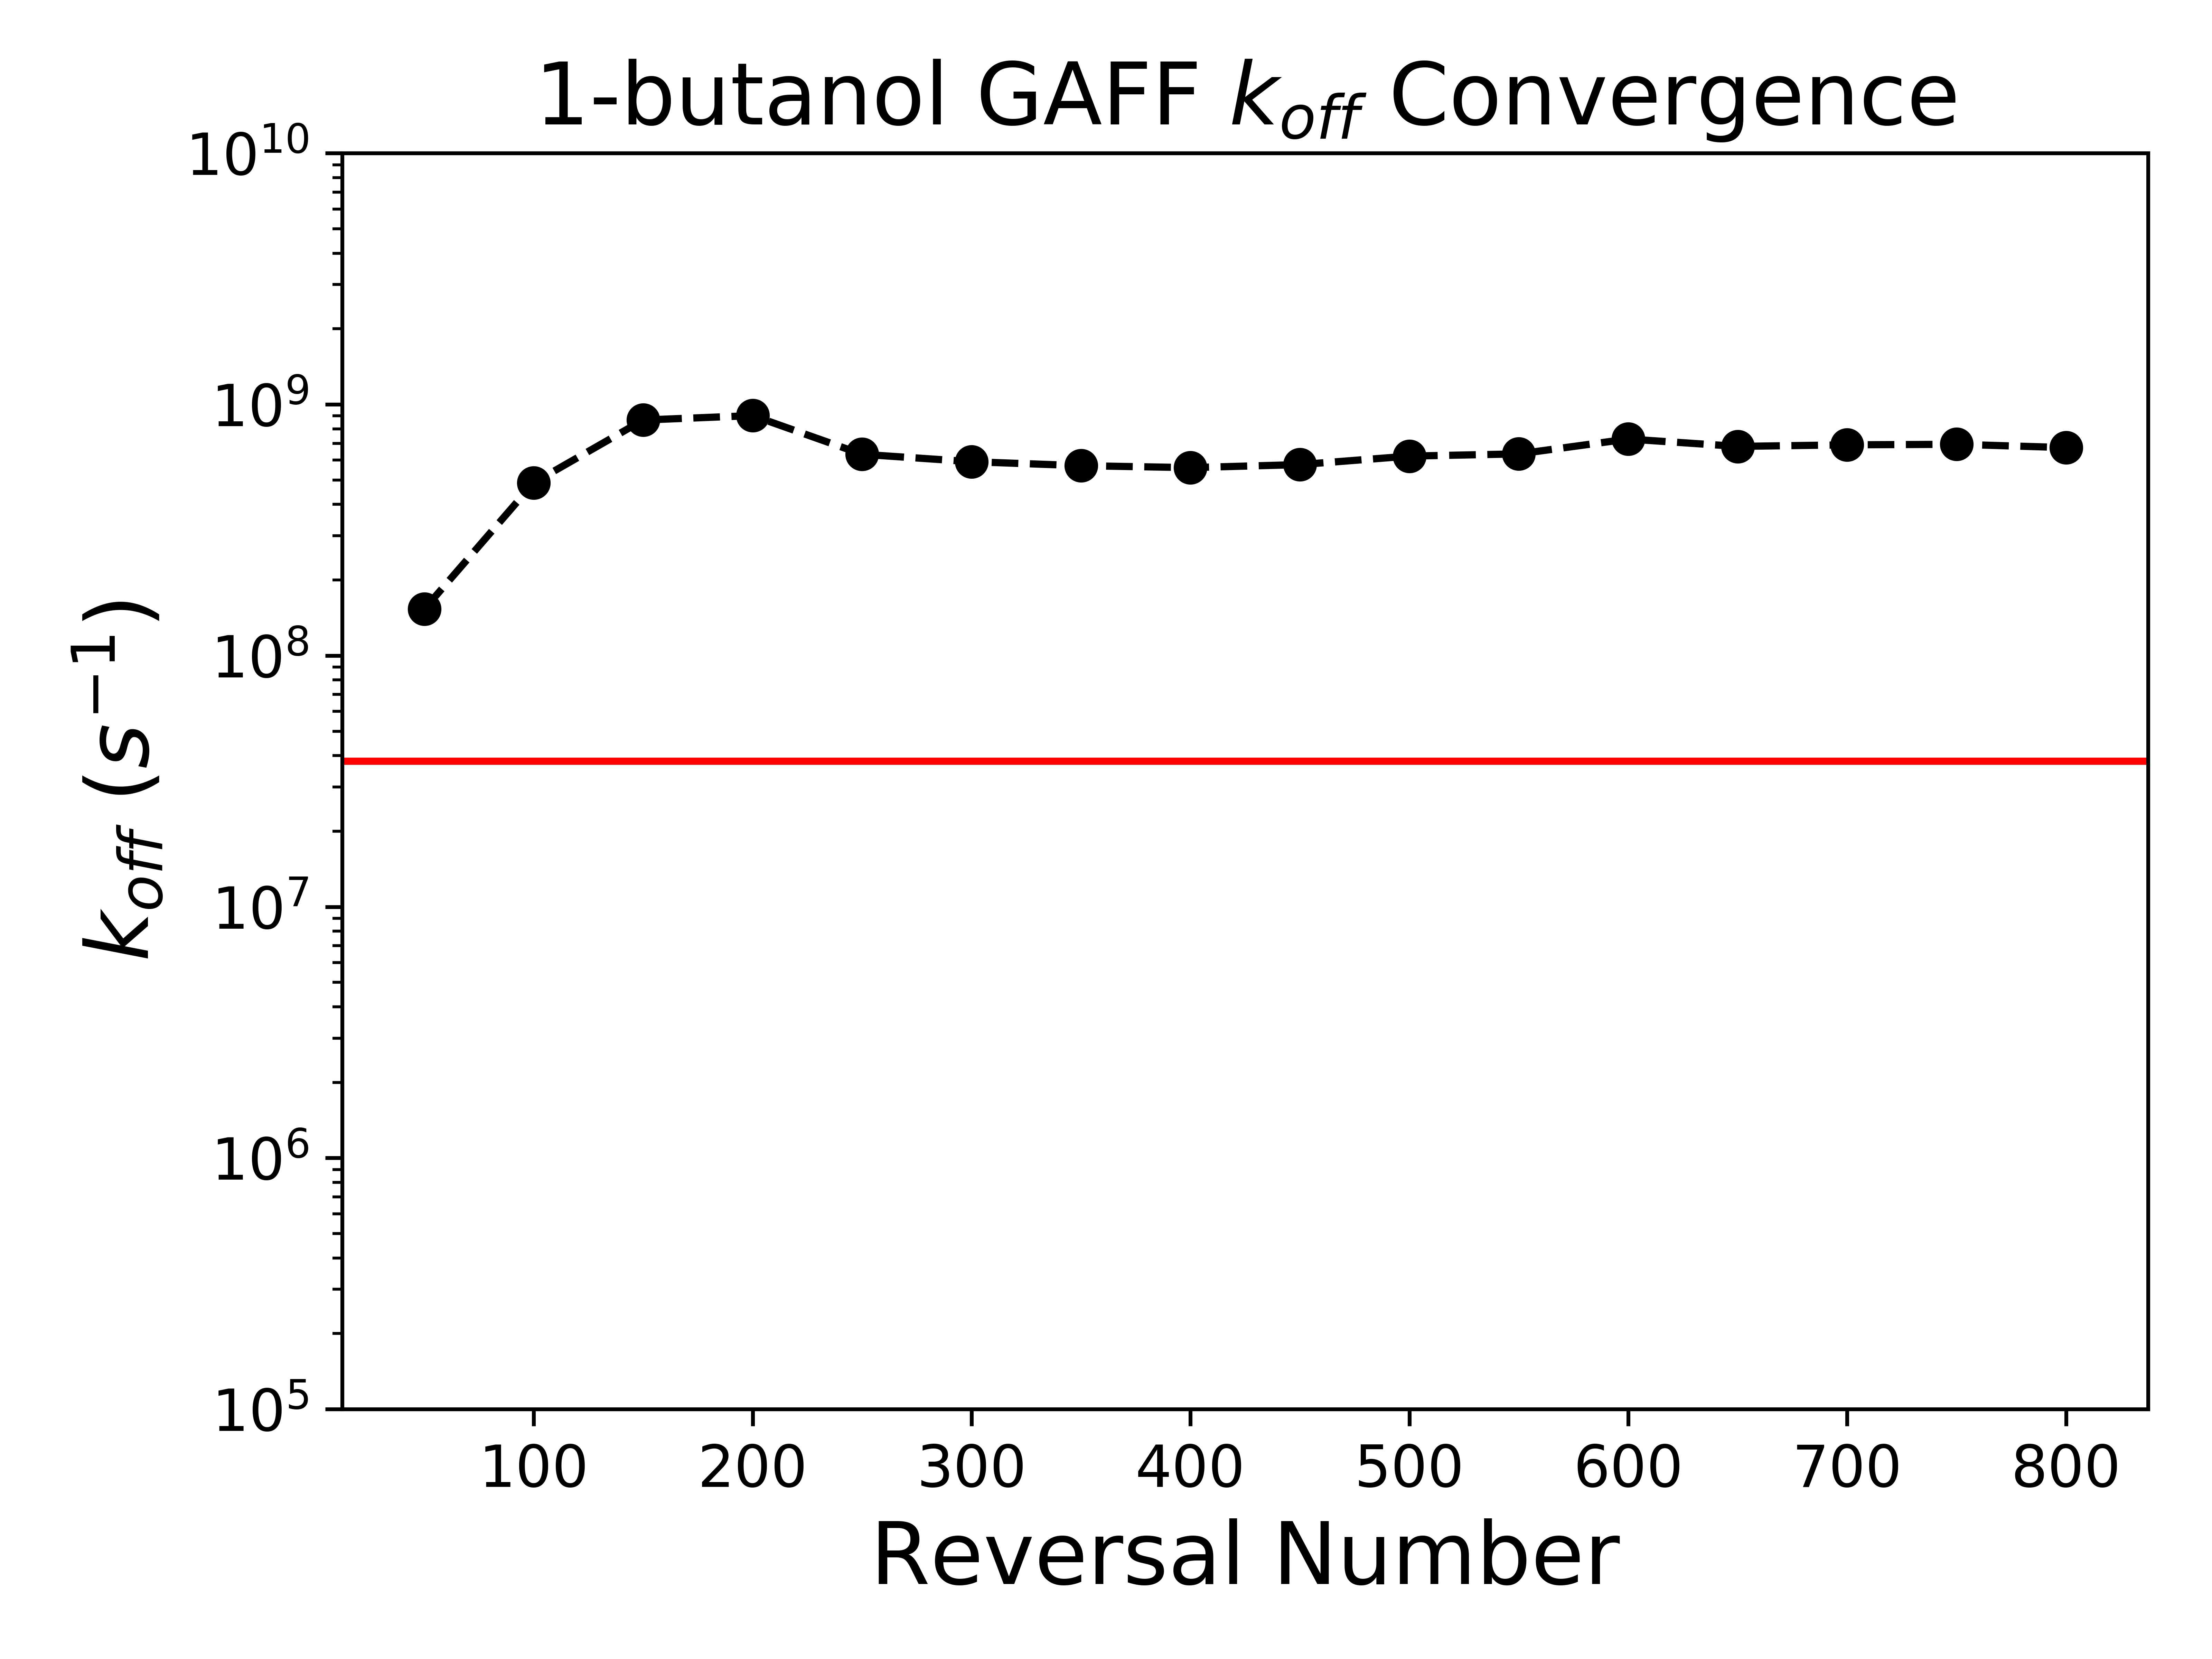
\includegraphics[width=\linewidth]{high_res_images/gaff_rate_conv_images/1-butanol_gaff_off_conv.png}
	\end{subfigure}%
	\begin{subfigure}{0.3\linewidth}
		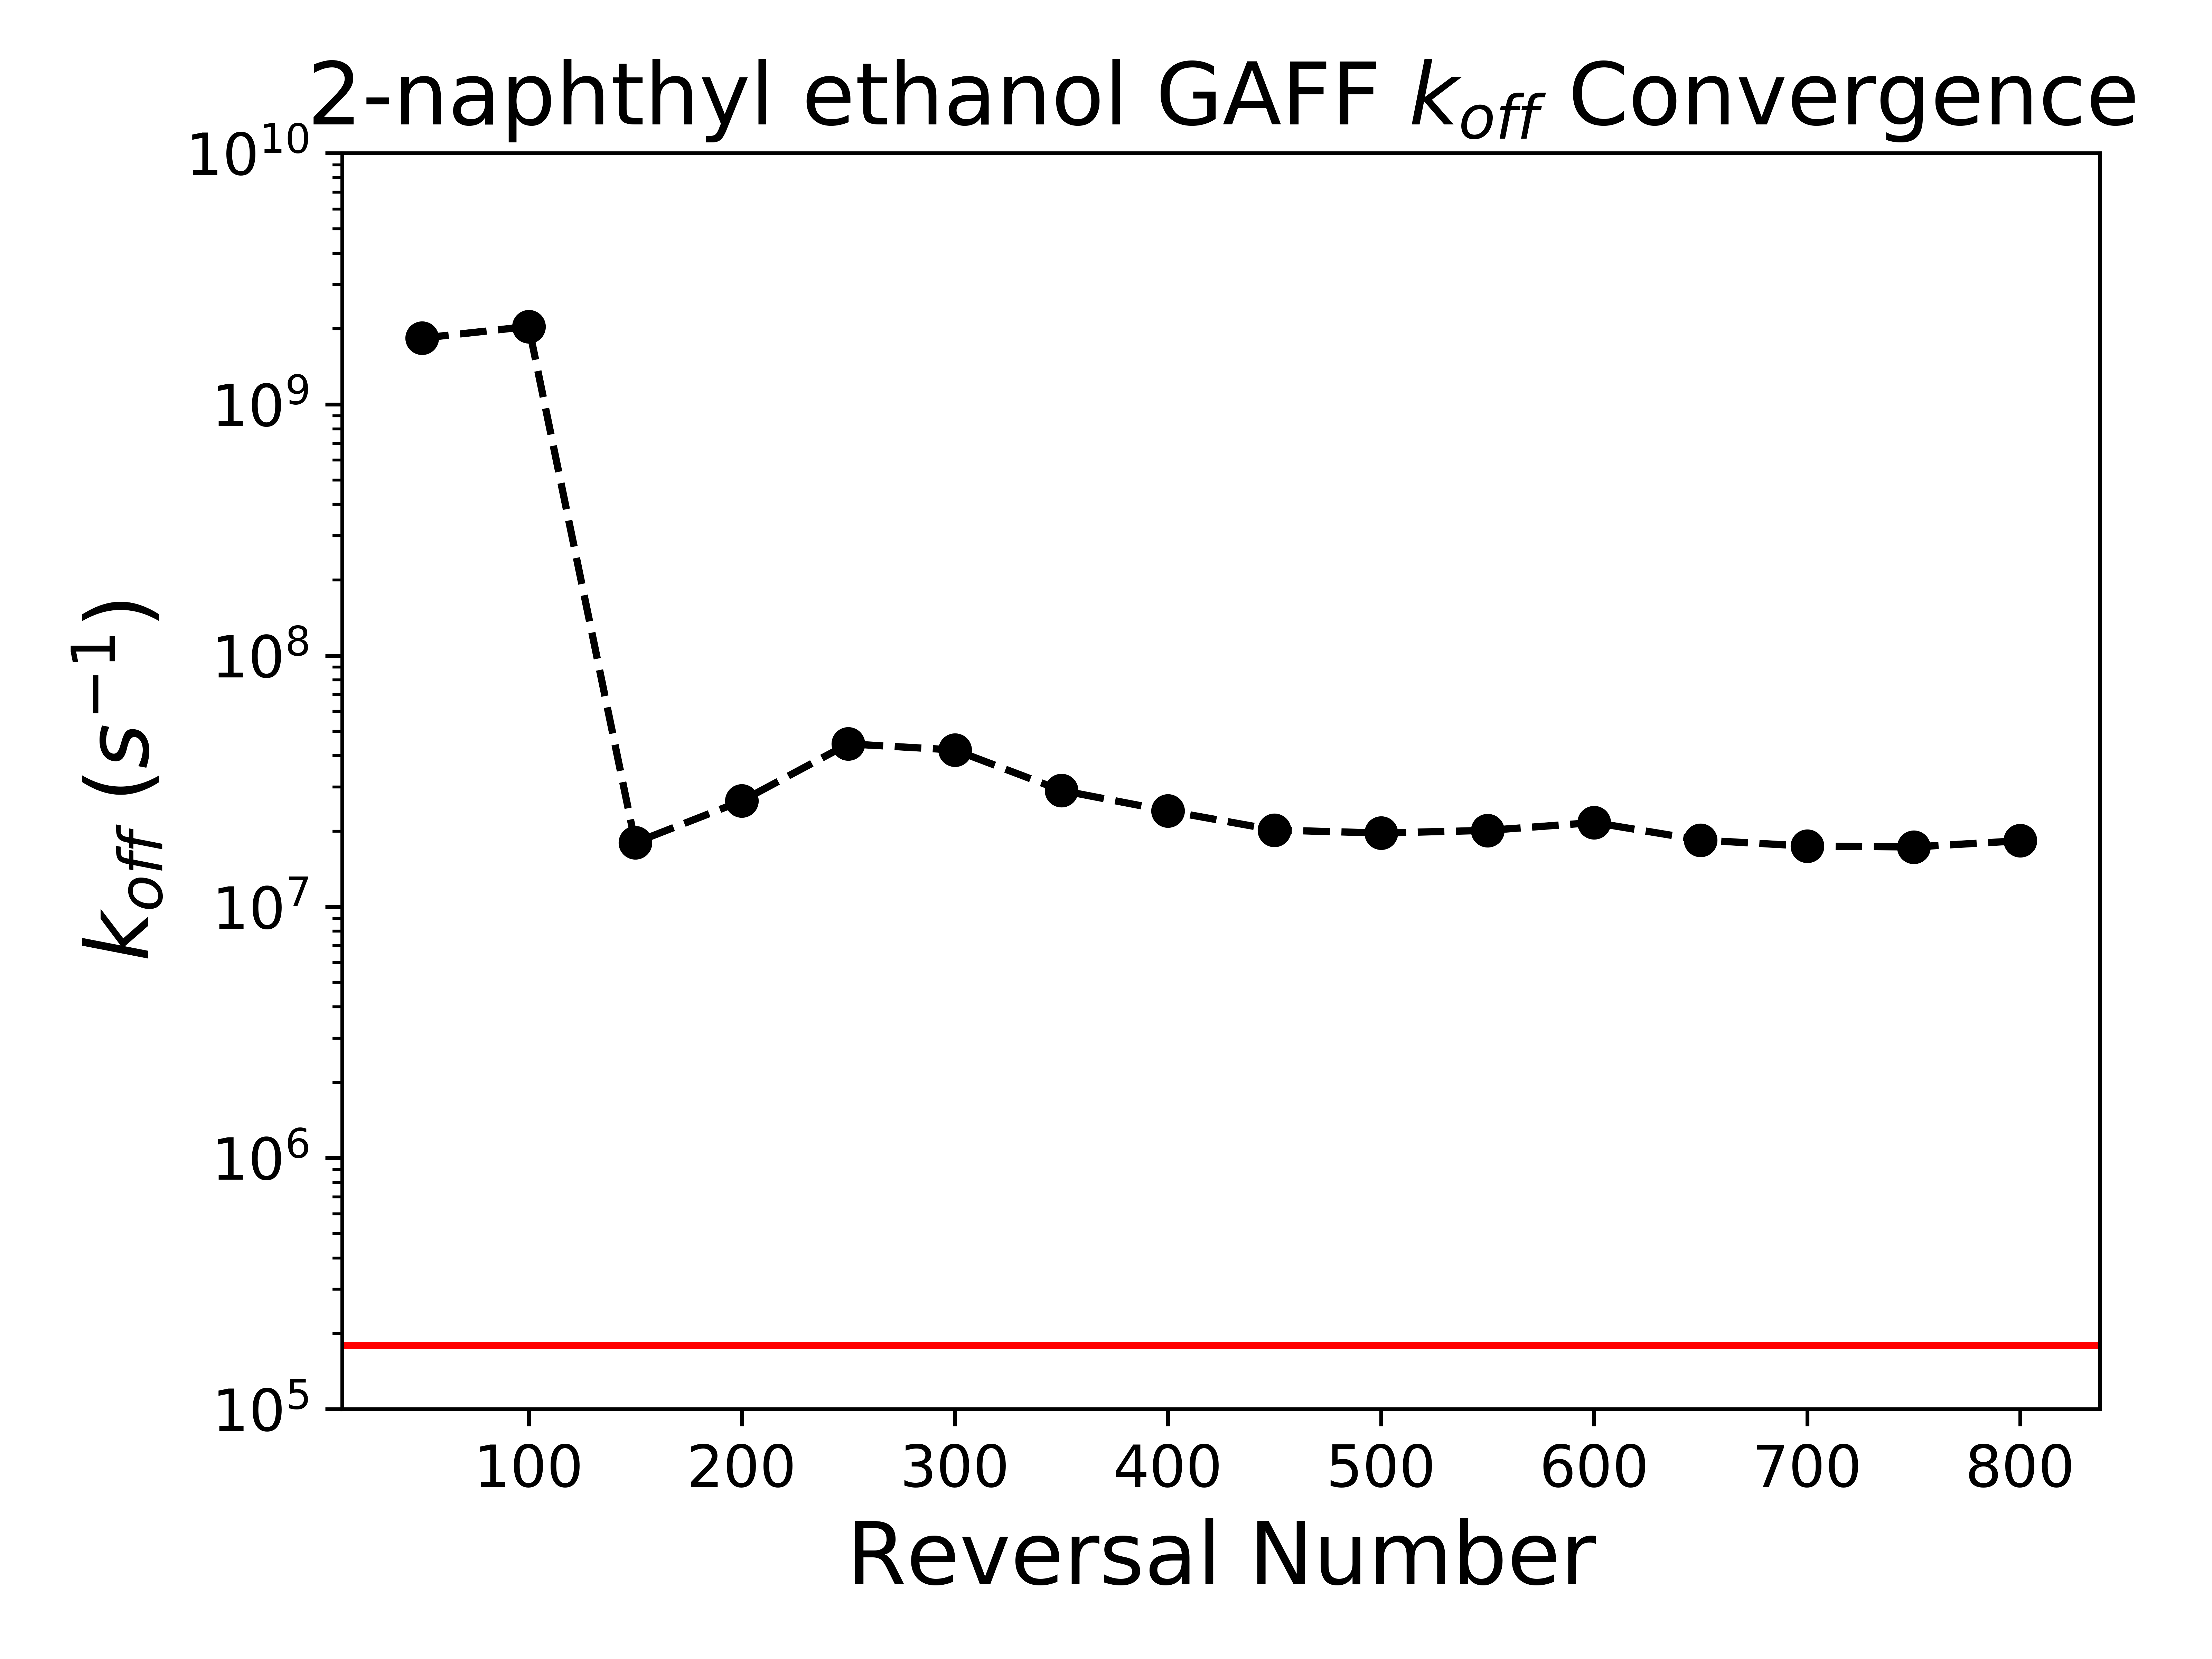
\includegraphics[width=\linewidth]{high_res_images/gaff_rate_conv_images/2-naphthylethanol_gaff_off_conv.png}
	\end{subfigure}%
	\begin{subfigure}{0.3\linewidth}
		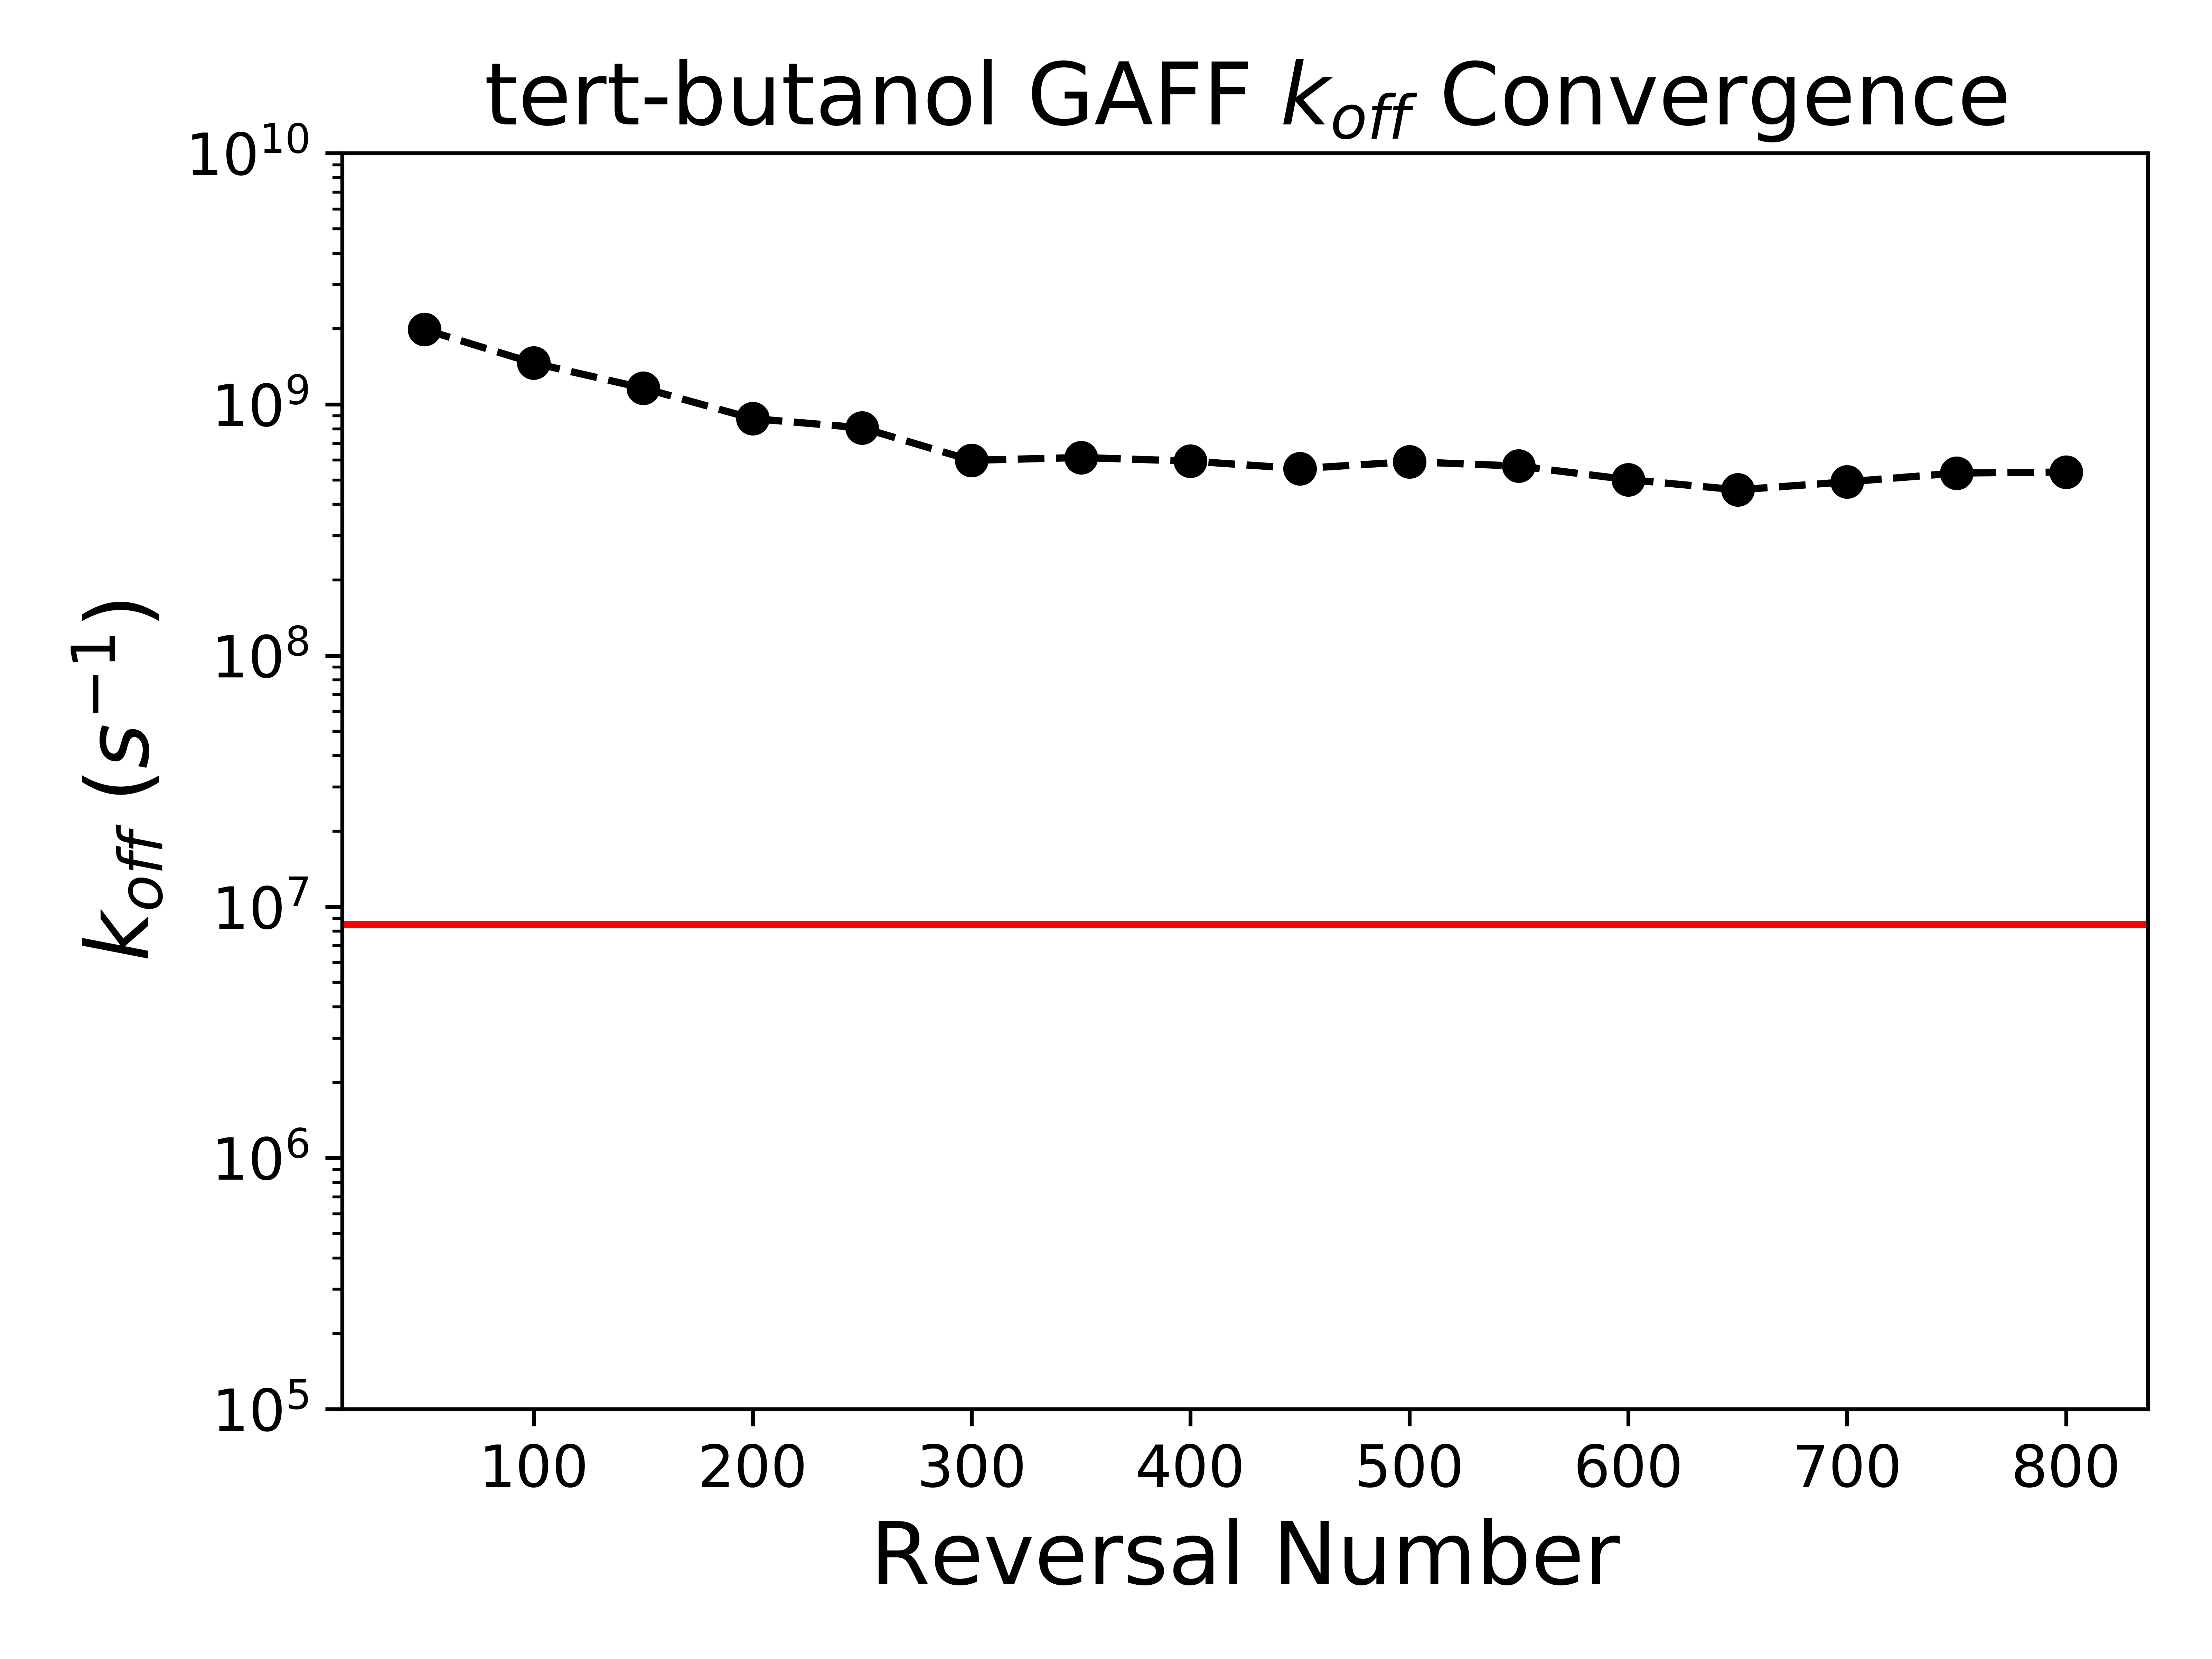
\includegraphics[width=\linewidth]{high_res_images/gaff_rate_conv_images/tert-butanol_gaff_off_conv.png}
	\end{subfigure}
	\begin{subfigure}{0.3\linewidth}
		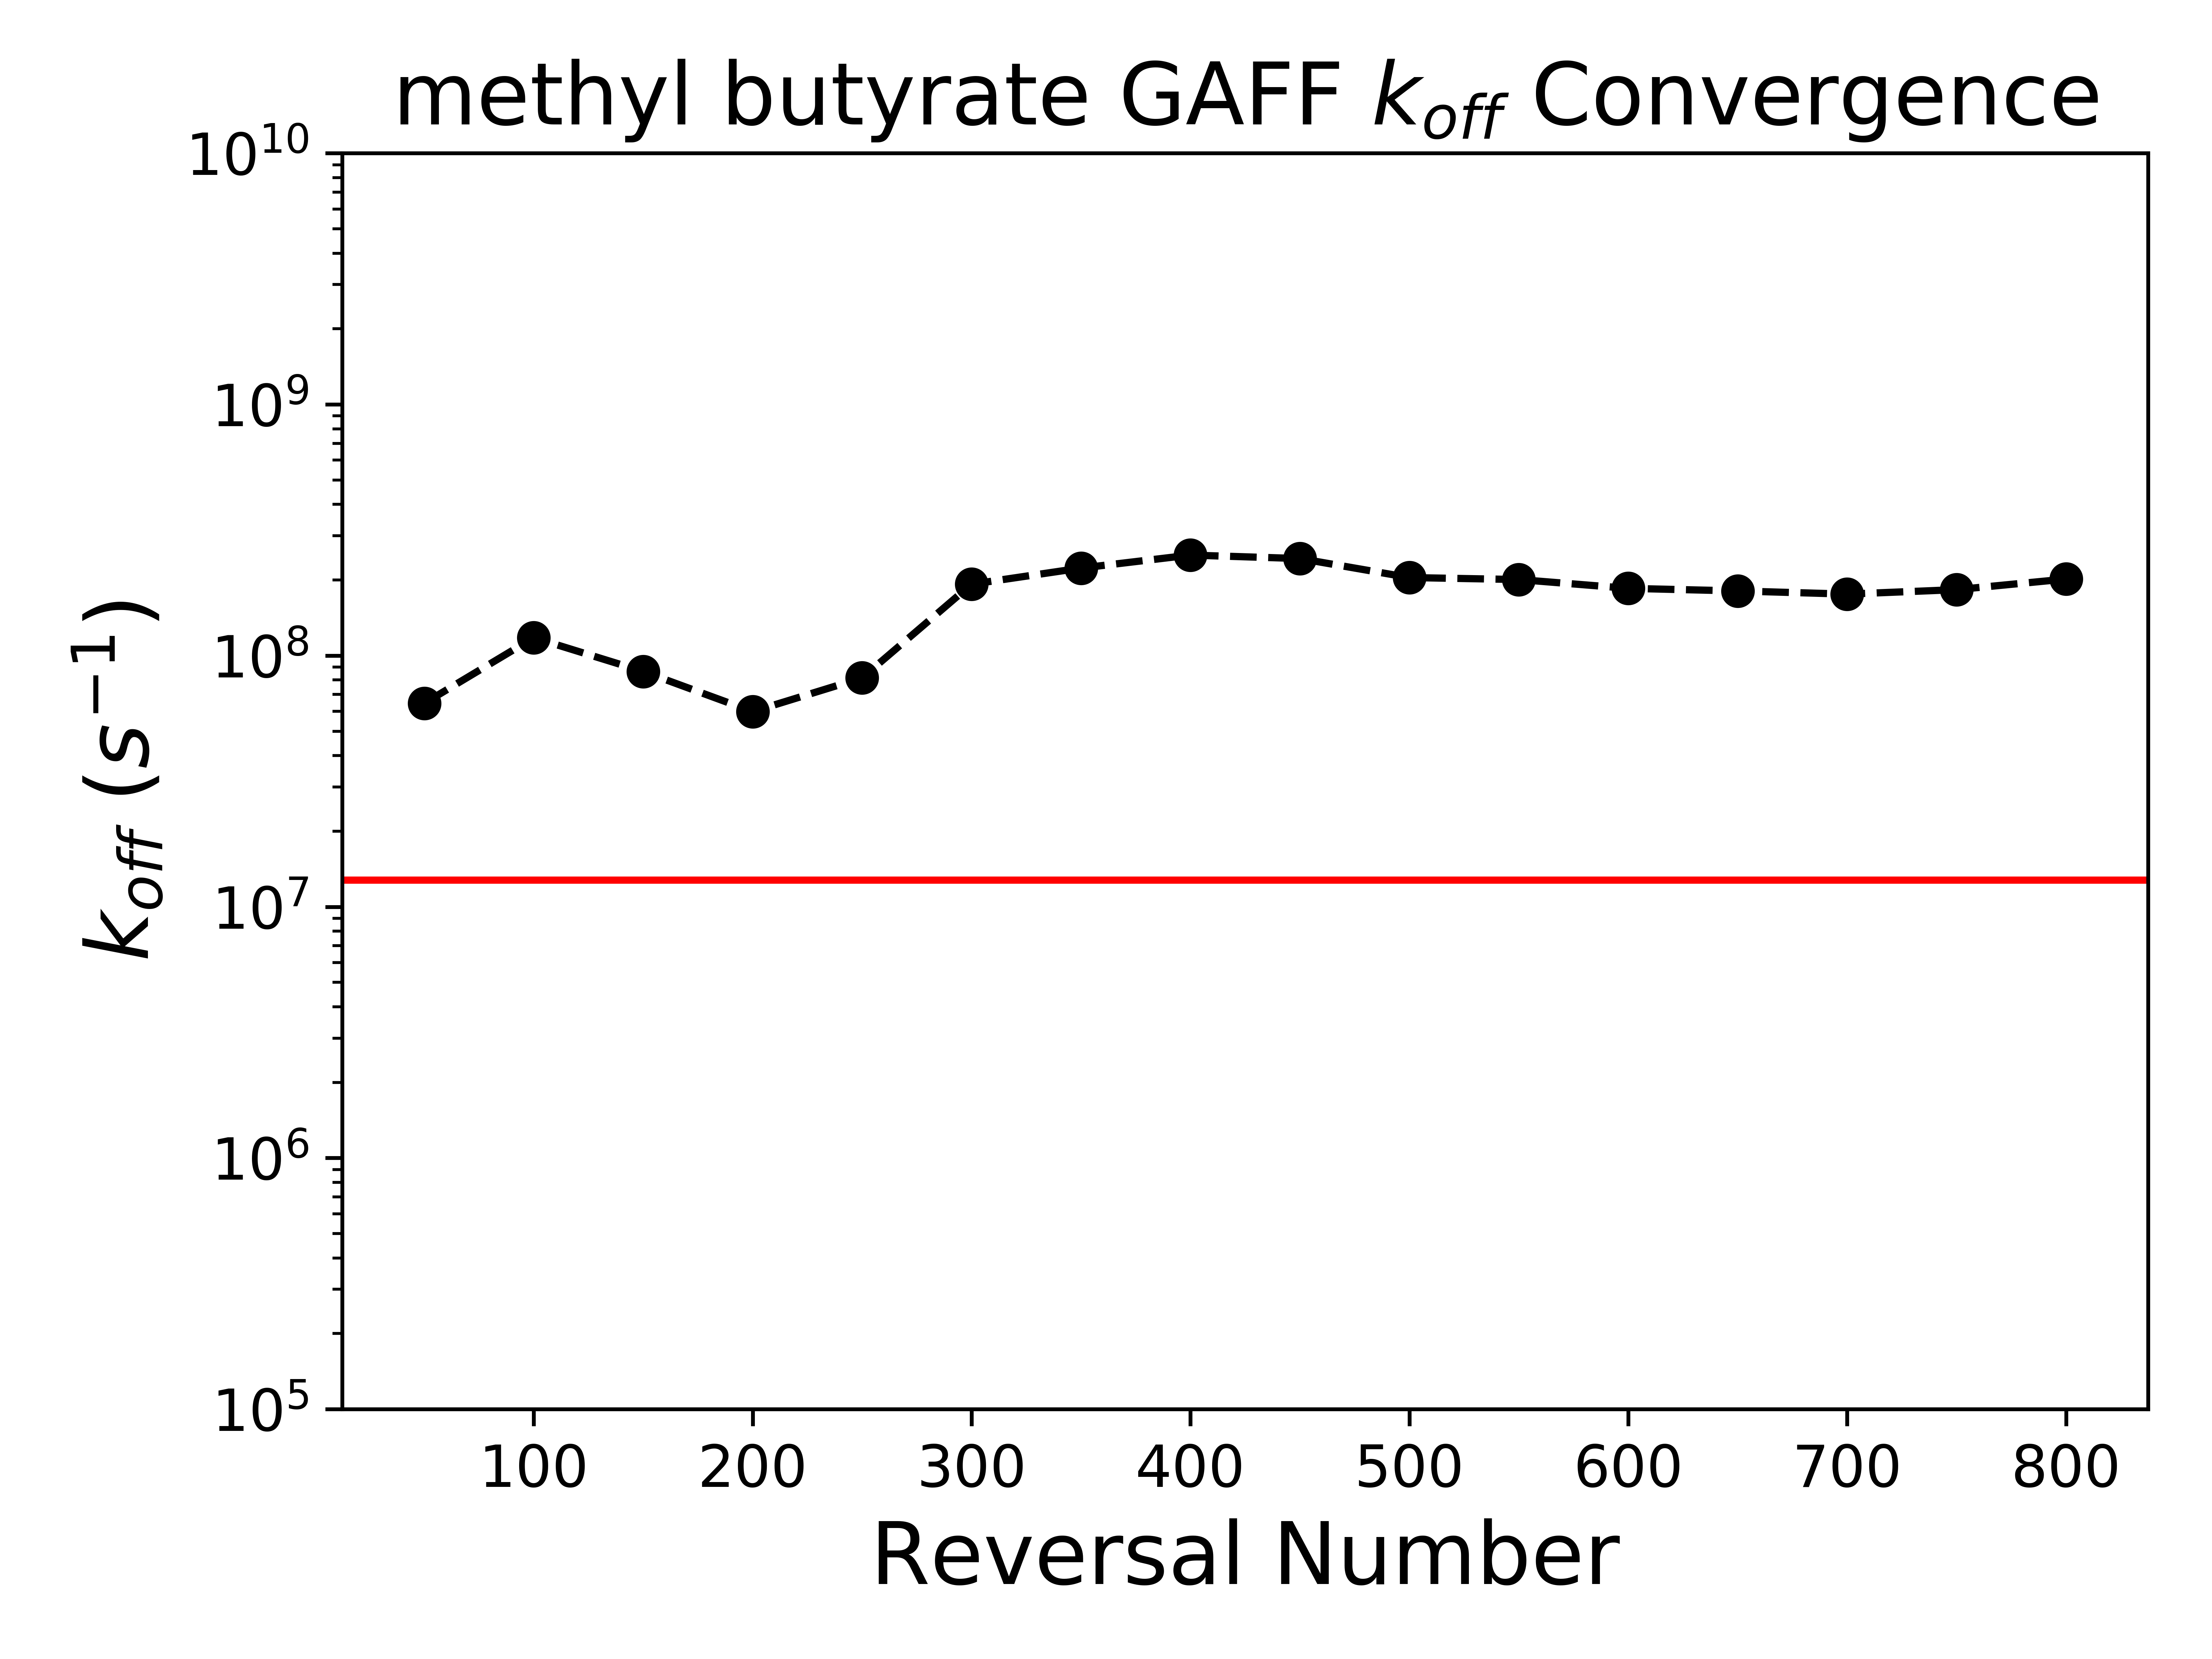
\includegraphics[width=\linewidth]{high_res_images/gaff_rate_conv_images/methylbutyrate_gaff_off_conv.png}
	\end{subfigure}
	\begin{subfigure}{0.3\linewidth}
		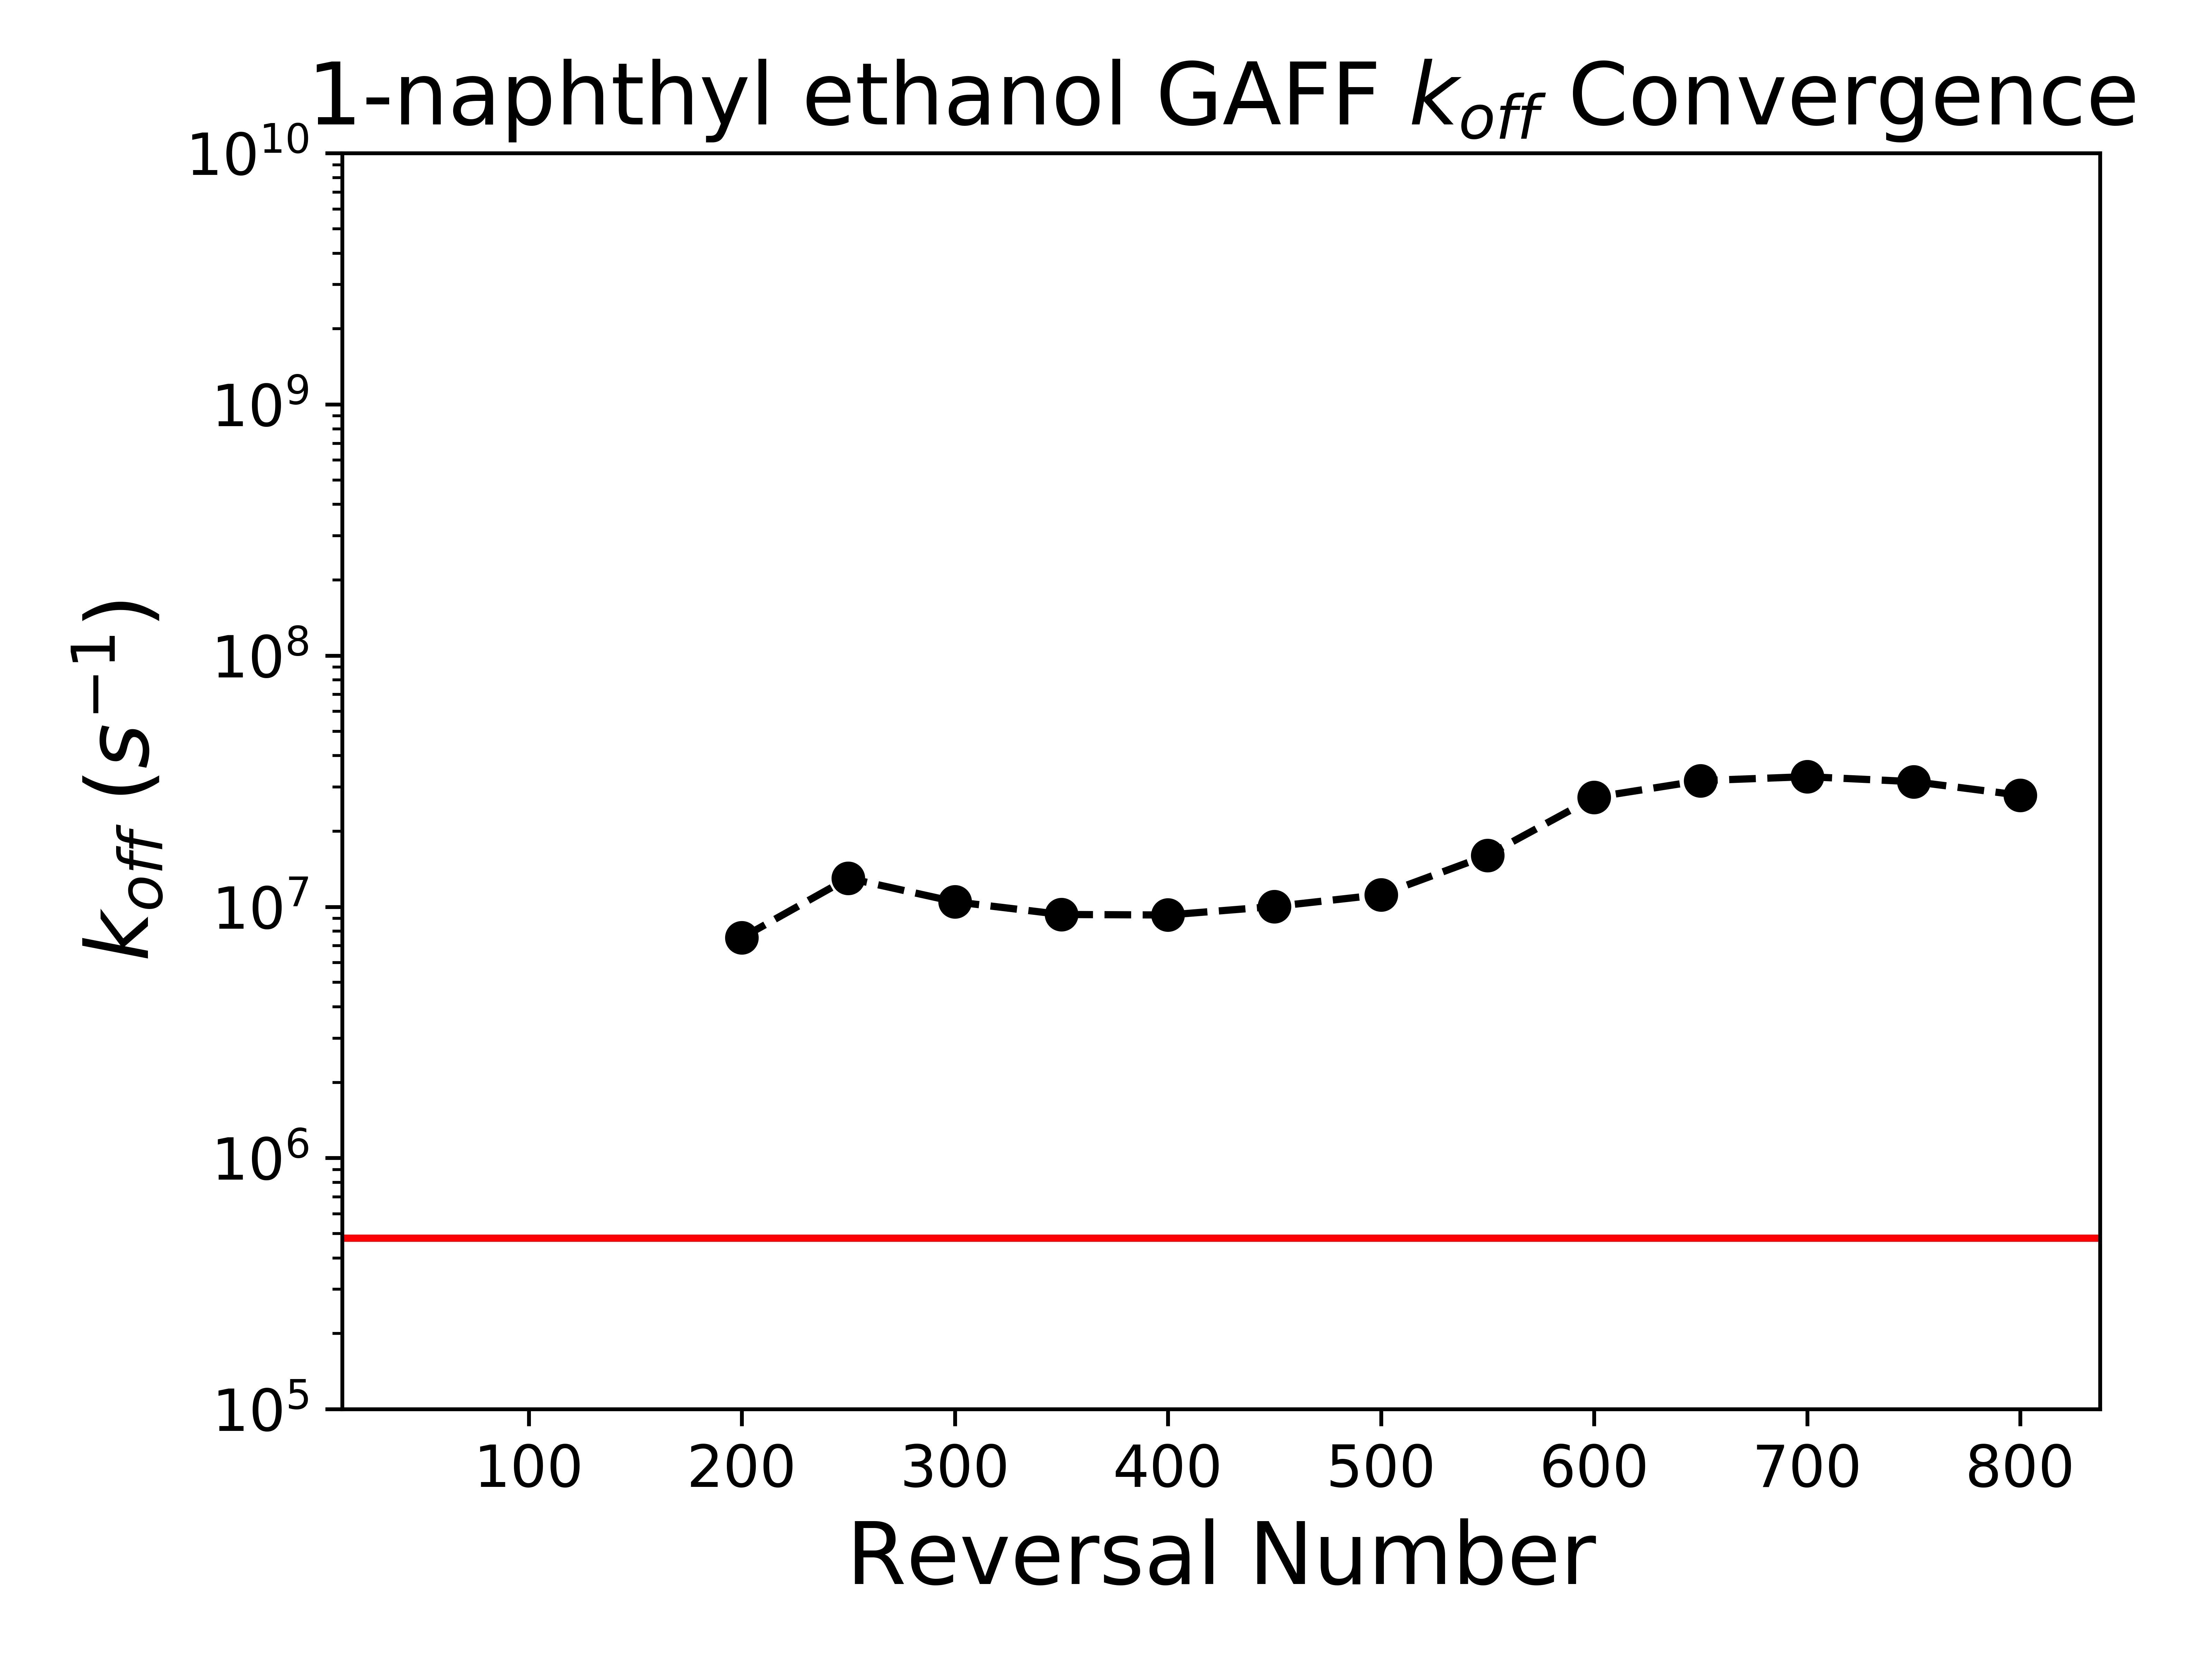
\includegraphics[width=\linewidth]{high_res_images/gaff_rate_conv_images/1-naphthylethanol_gaff_off_conv.png}
	\end{subfigure}
	\begin{subfigure}{0.3\linewidth}
		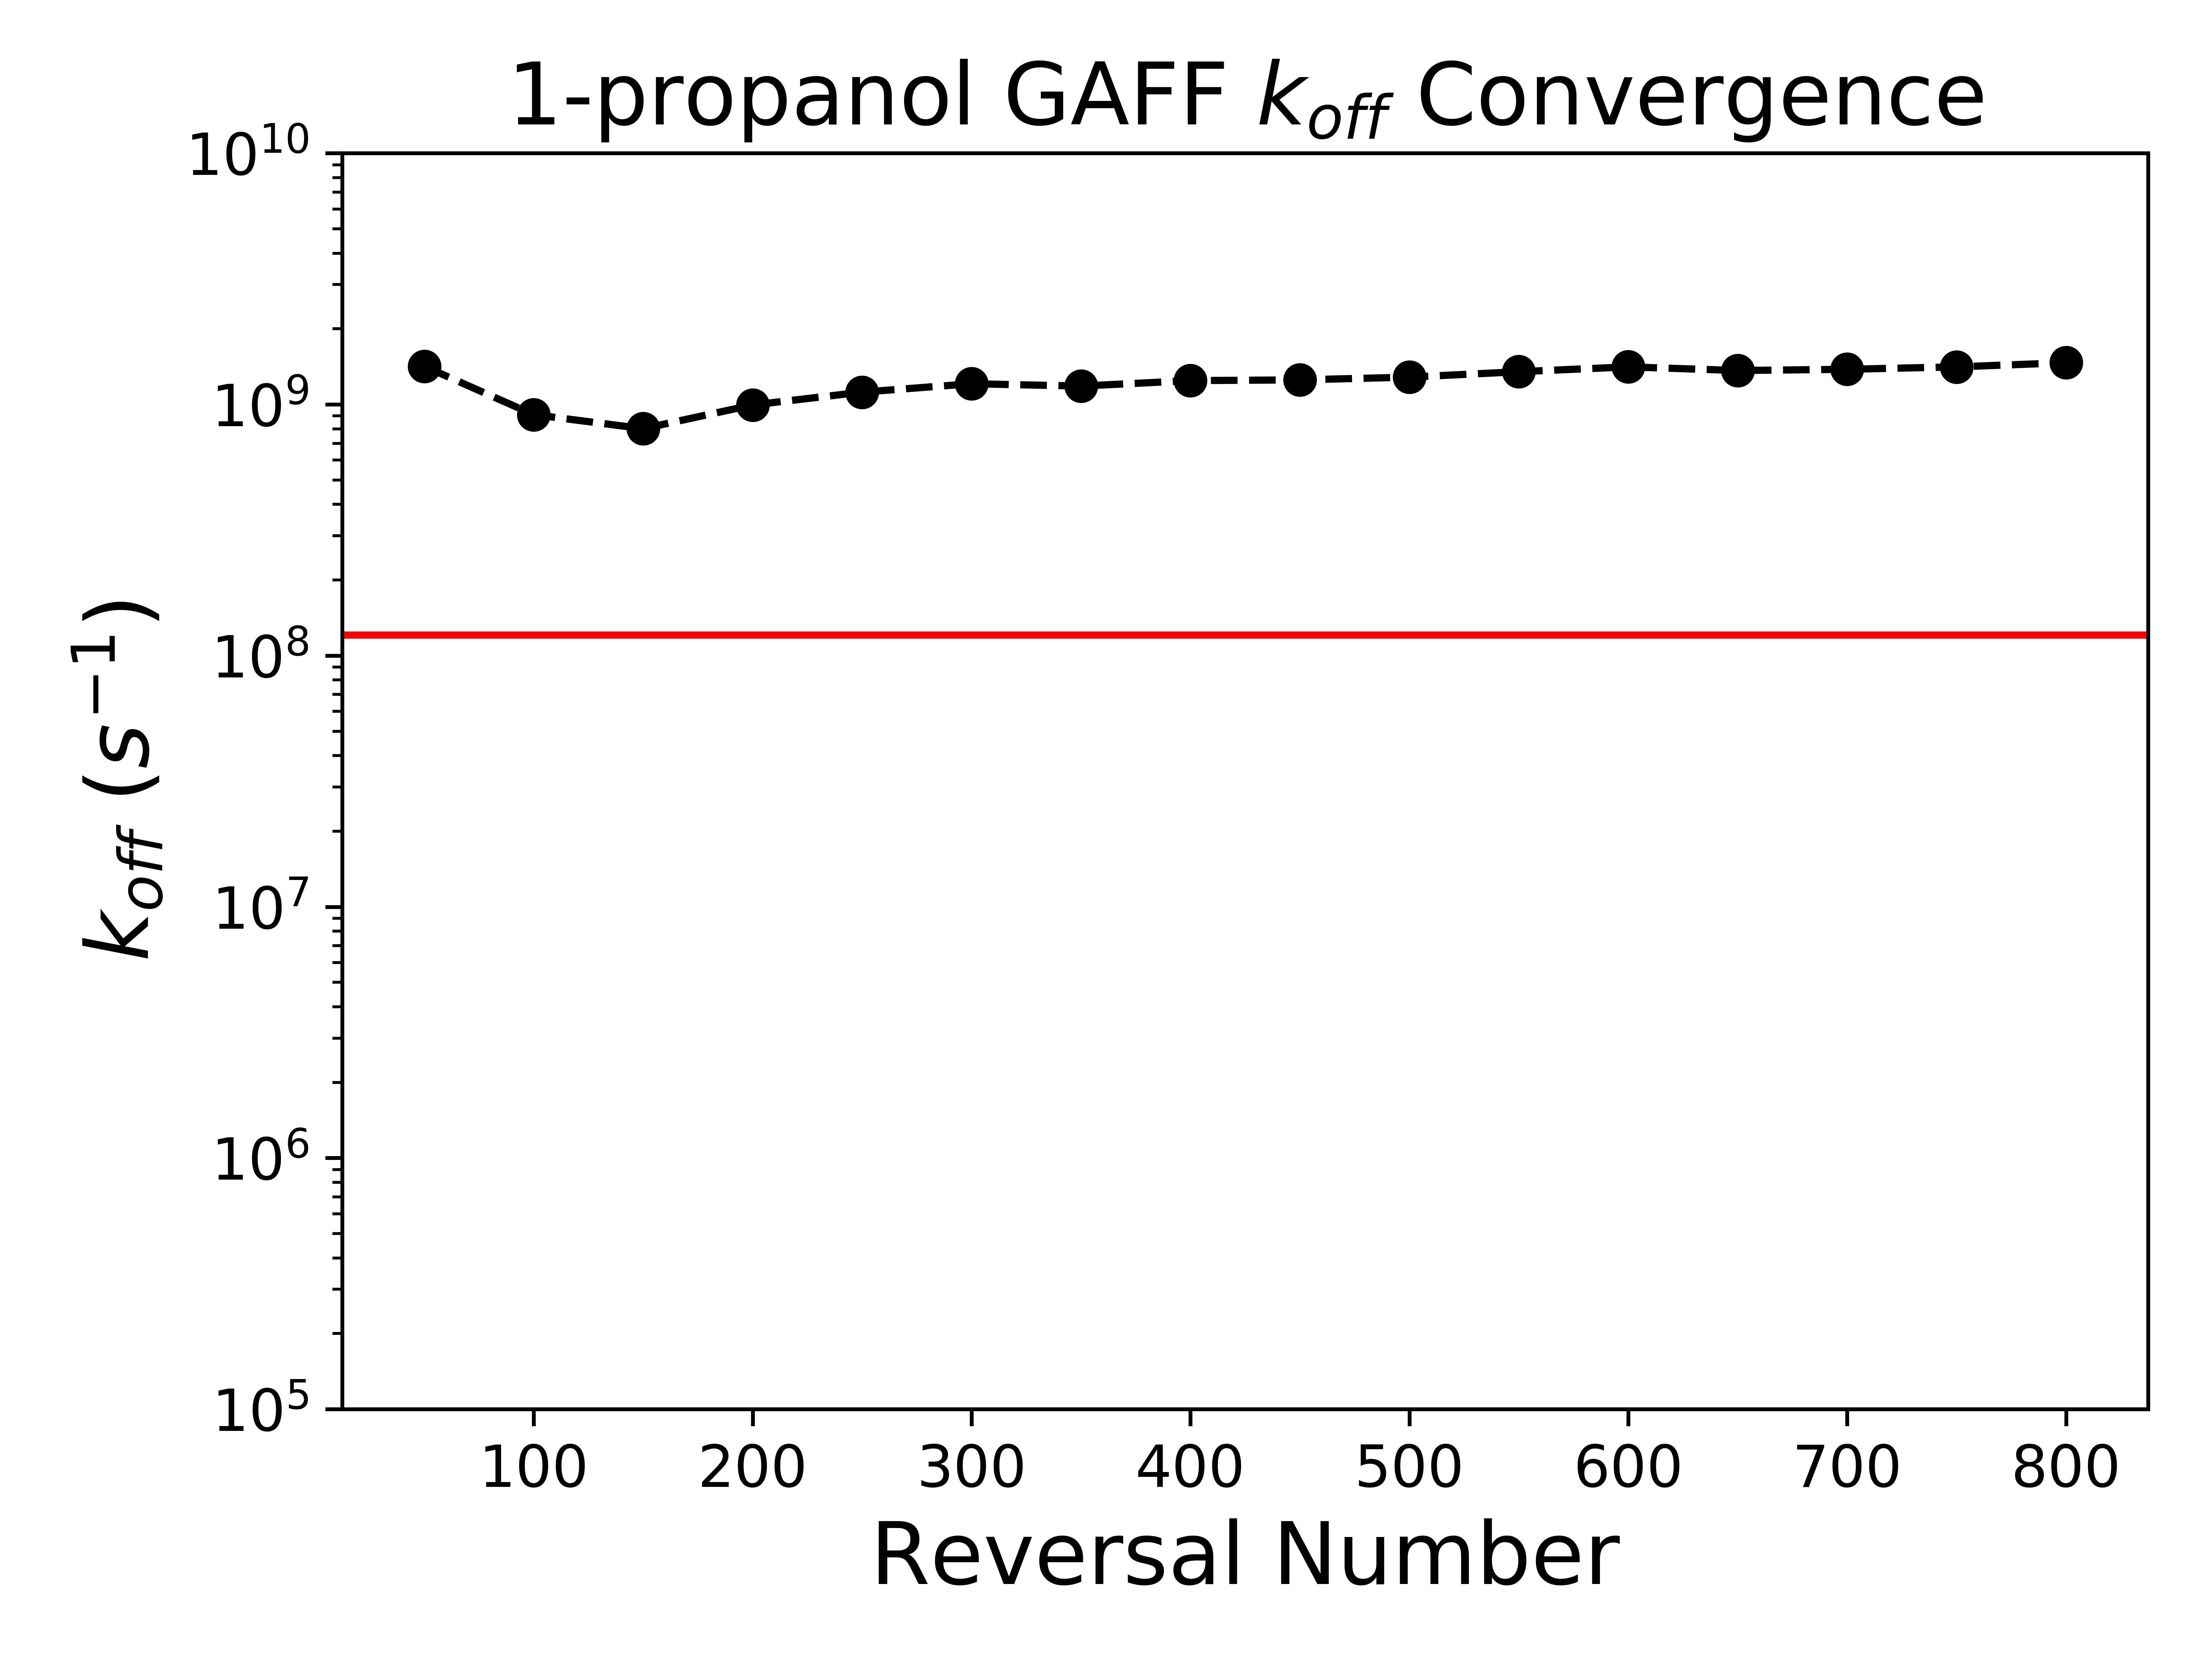
\includegraphics[width=\linewidth]{high_res_images/gaff_rate_conv_images/1-propanol_gaff_off_conv.png}
	\end{subfigure}
	\begin{subfigure}{0.3\linewidth}
		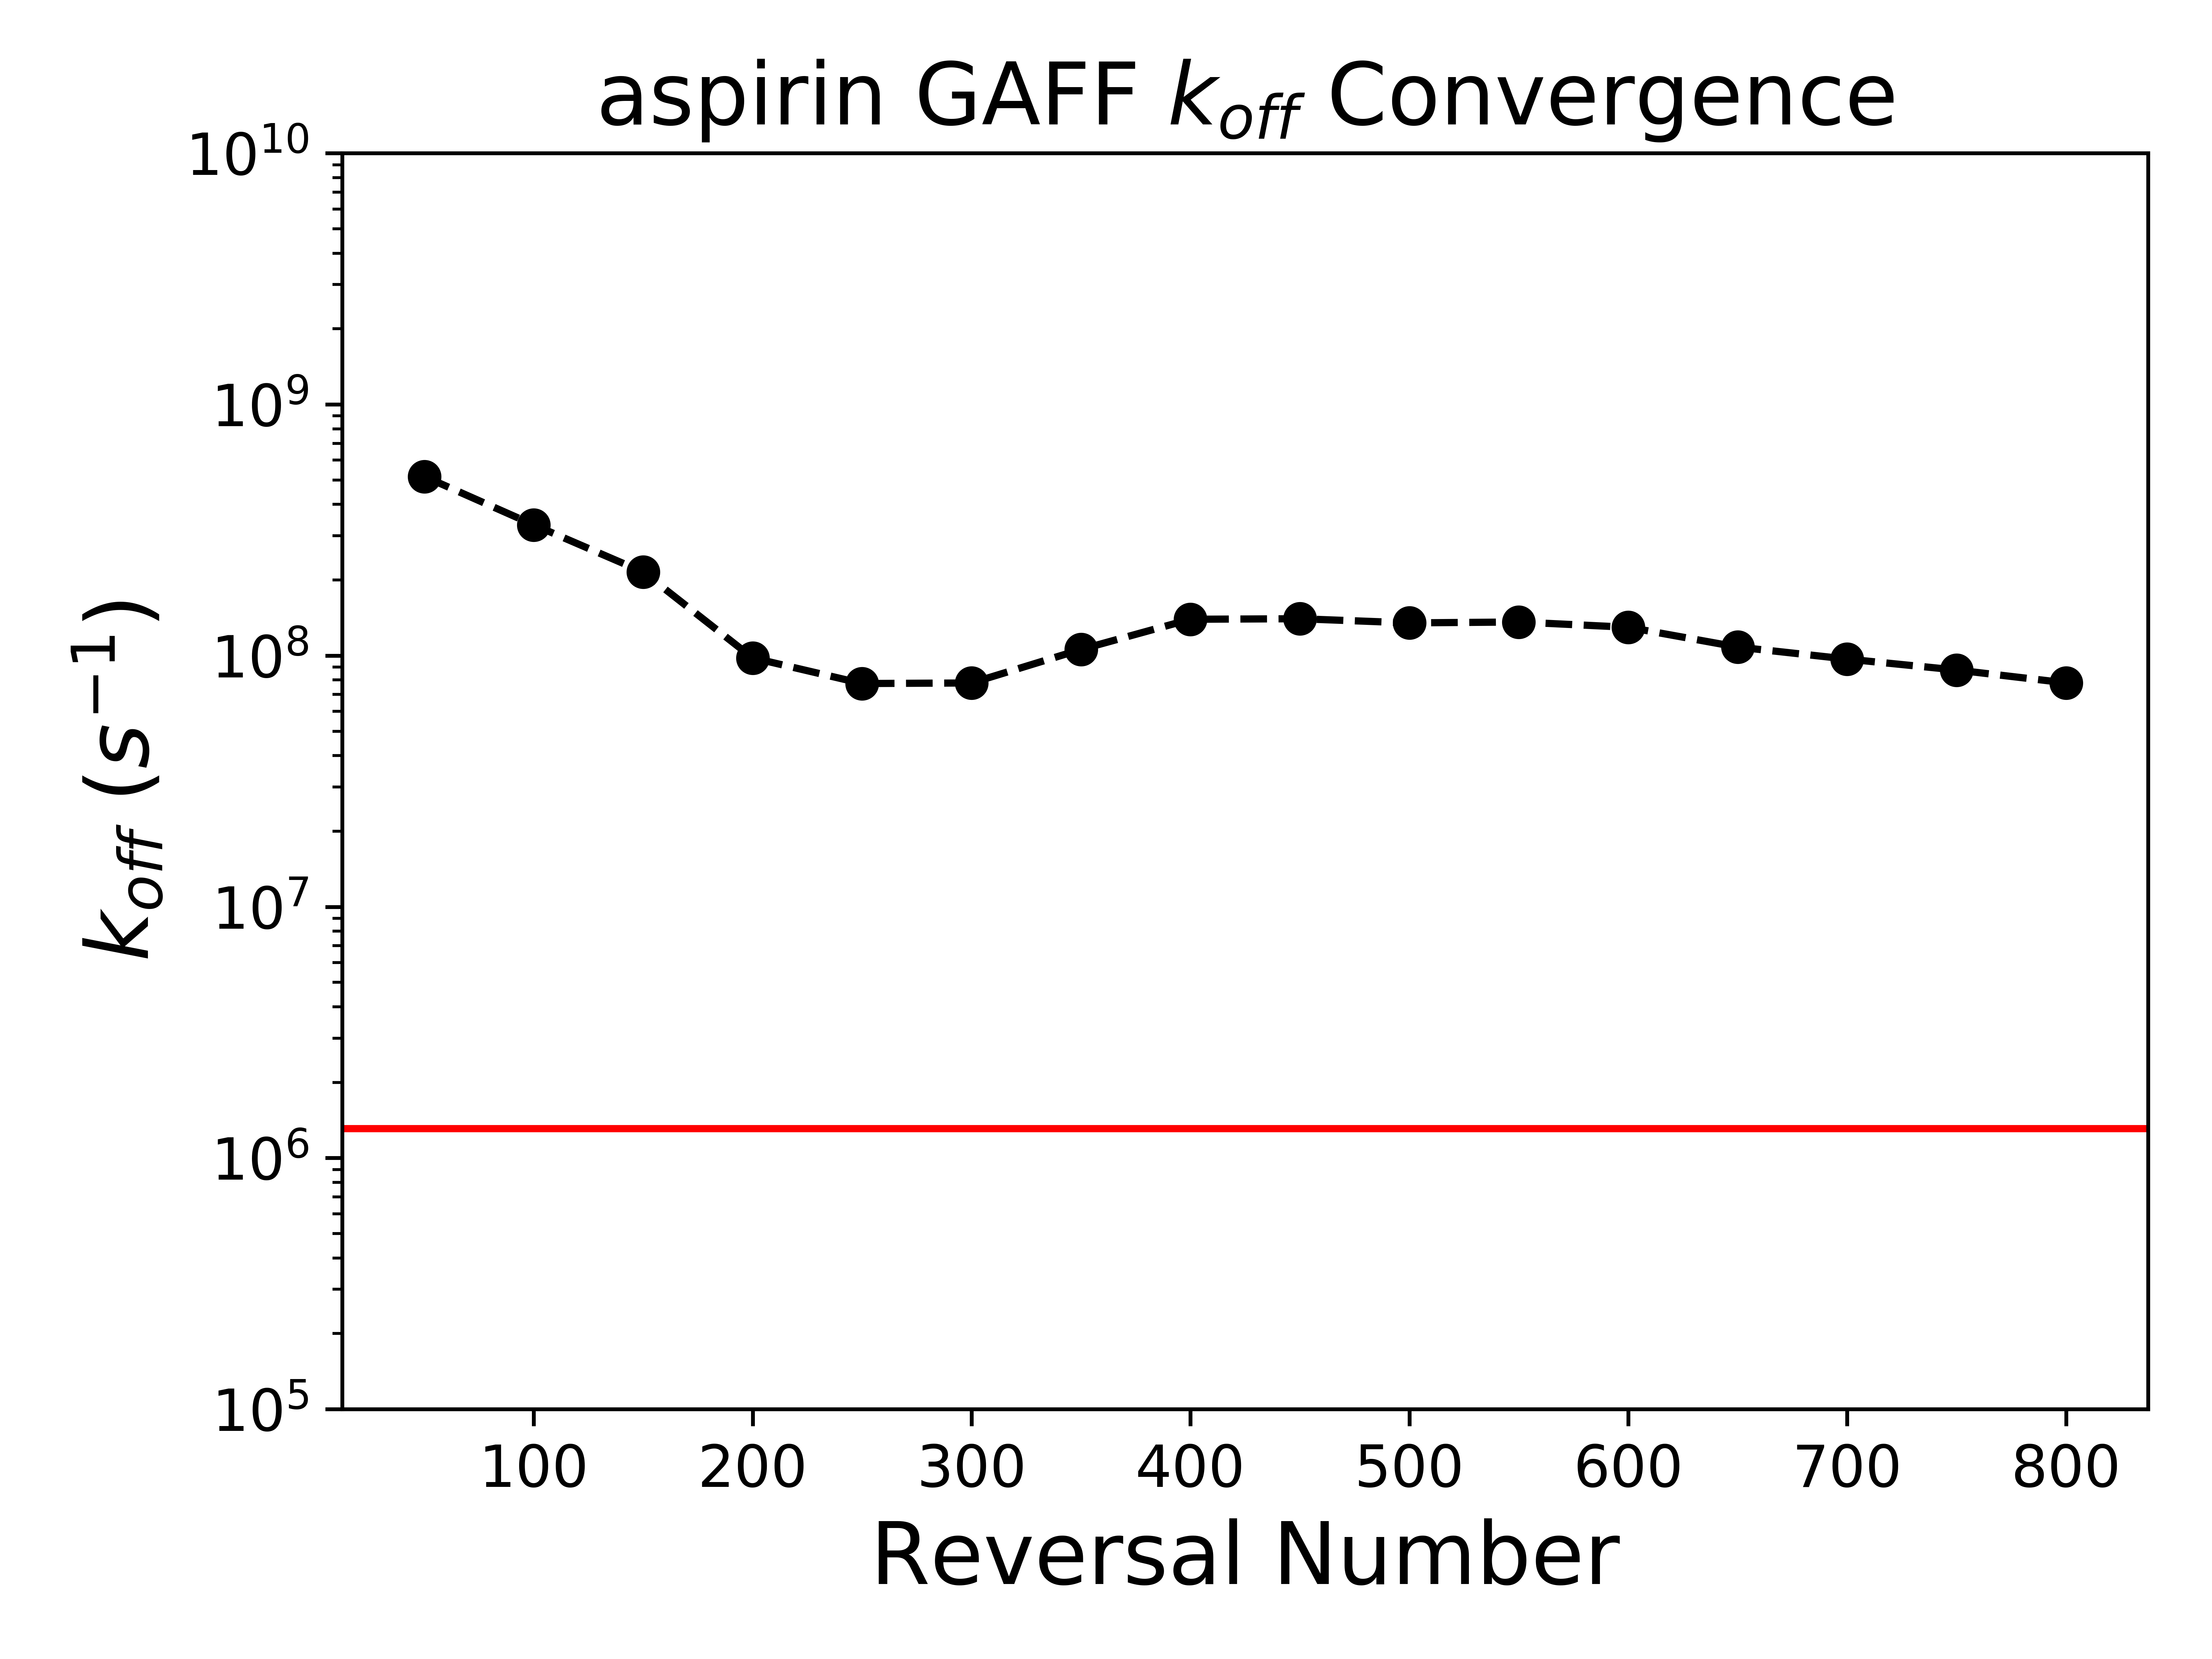
\includegraphics[width=\linewidth]{high_res_images/gaff_rate_conv_images/aspirin_gaff_off_conv.png}
	\end{subfigure}
	\caption{Convergence of off rates as a function of the number of reversals included using the GAFF forcefield}
\end{figure}
%\begin{figure}
\begin{subfigure}{0.3\linewidth}
	\centering
	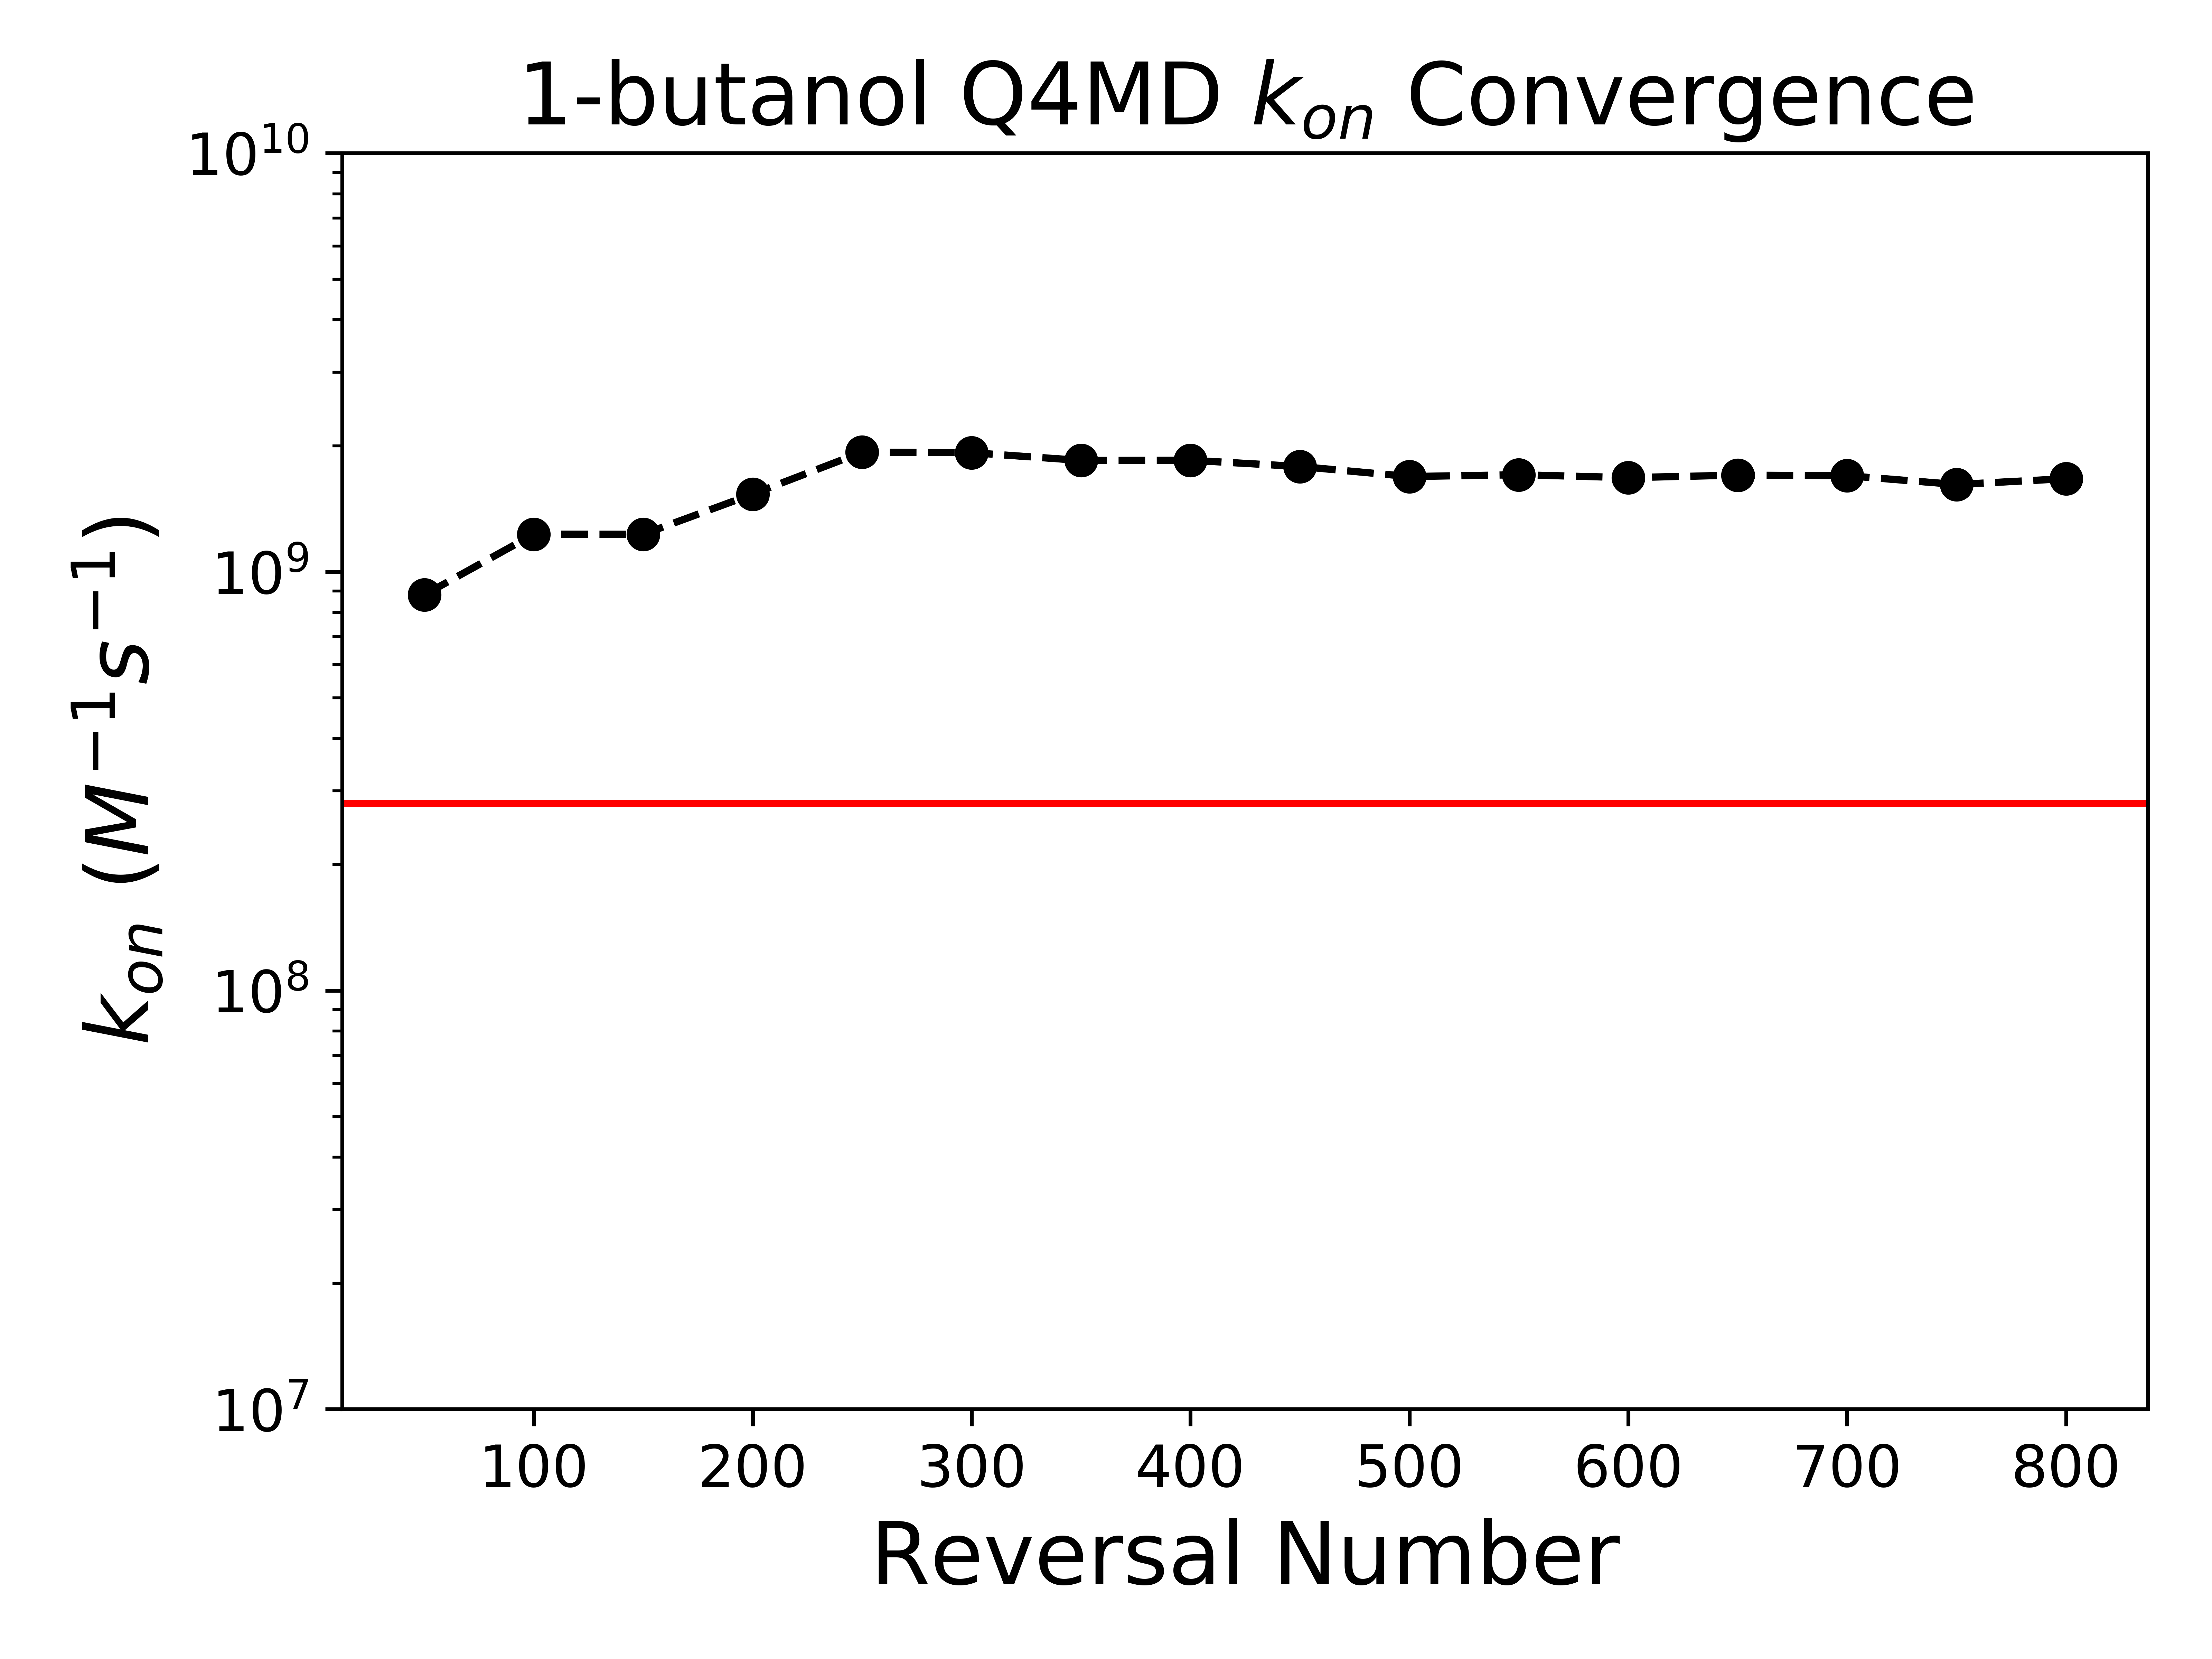
\includegraphics[width=\linewidth]{high_res_images/q4md_rate_conv_images/1-butanol_q4md_on_conv.png}
	\end{subfigure}%
\begin{subfigure}{0.3\linewidth}
		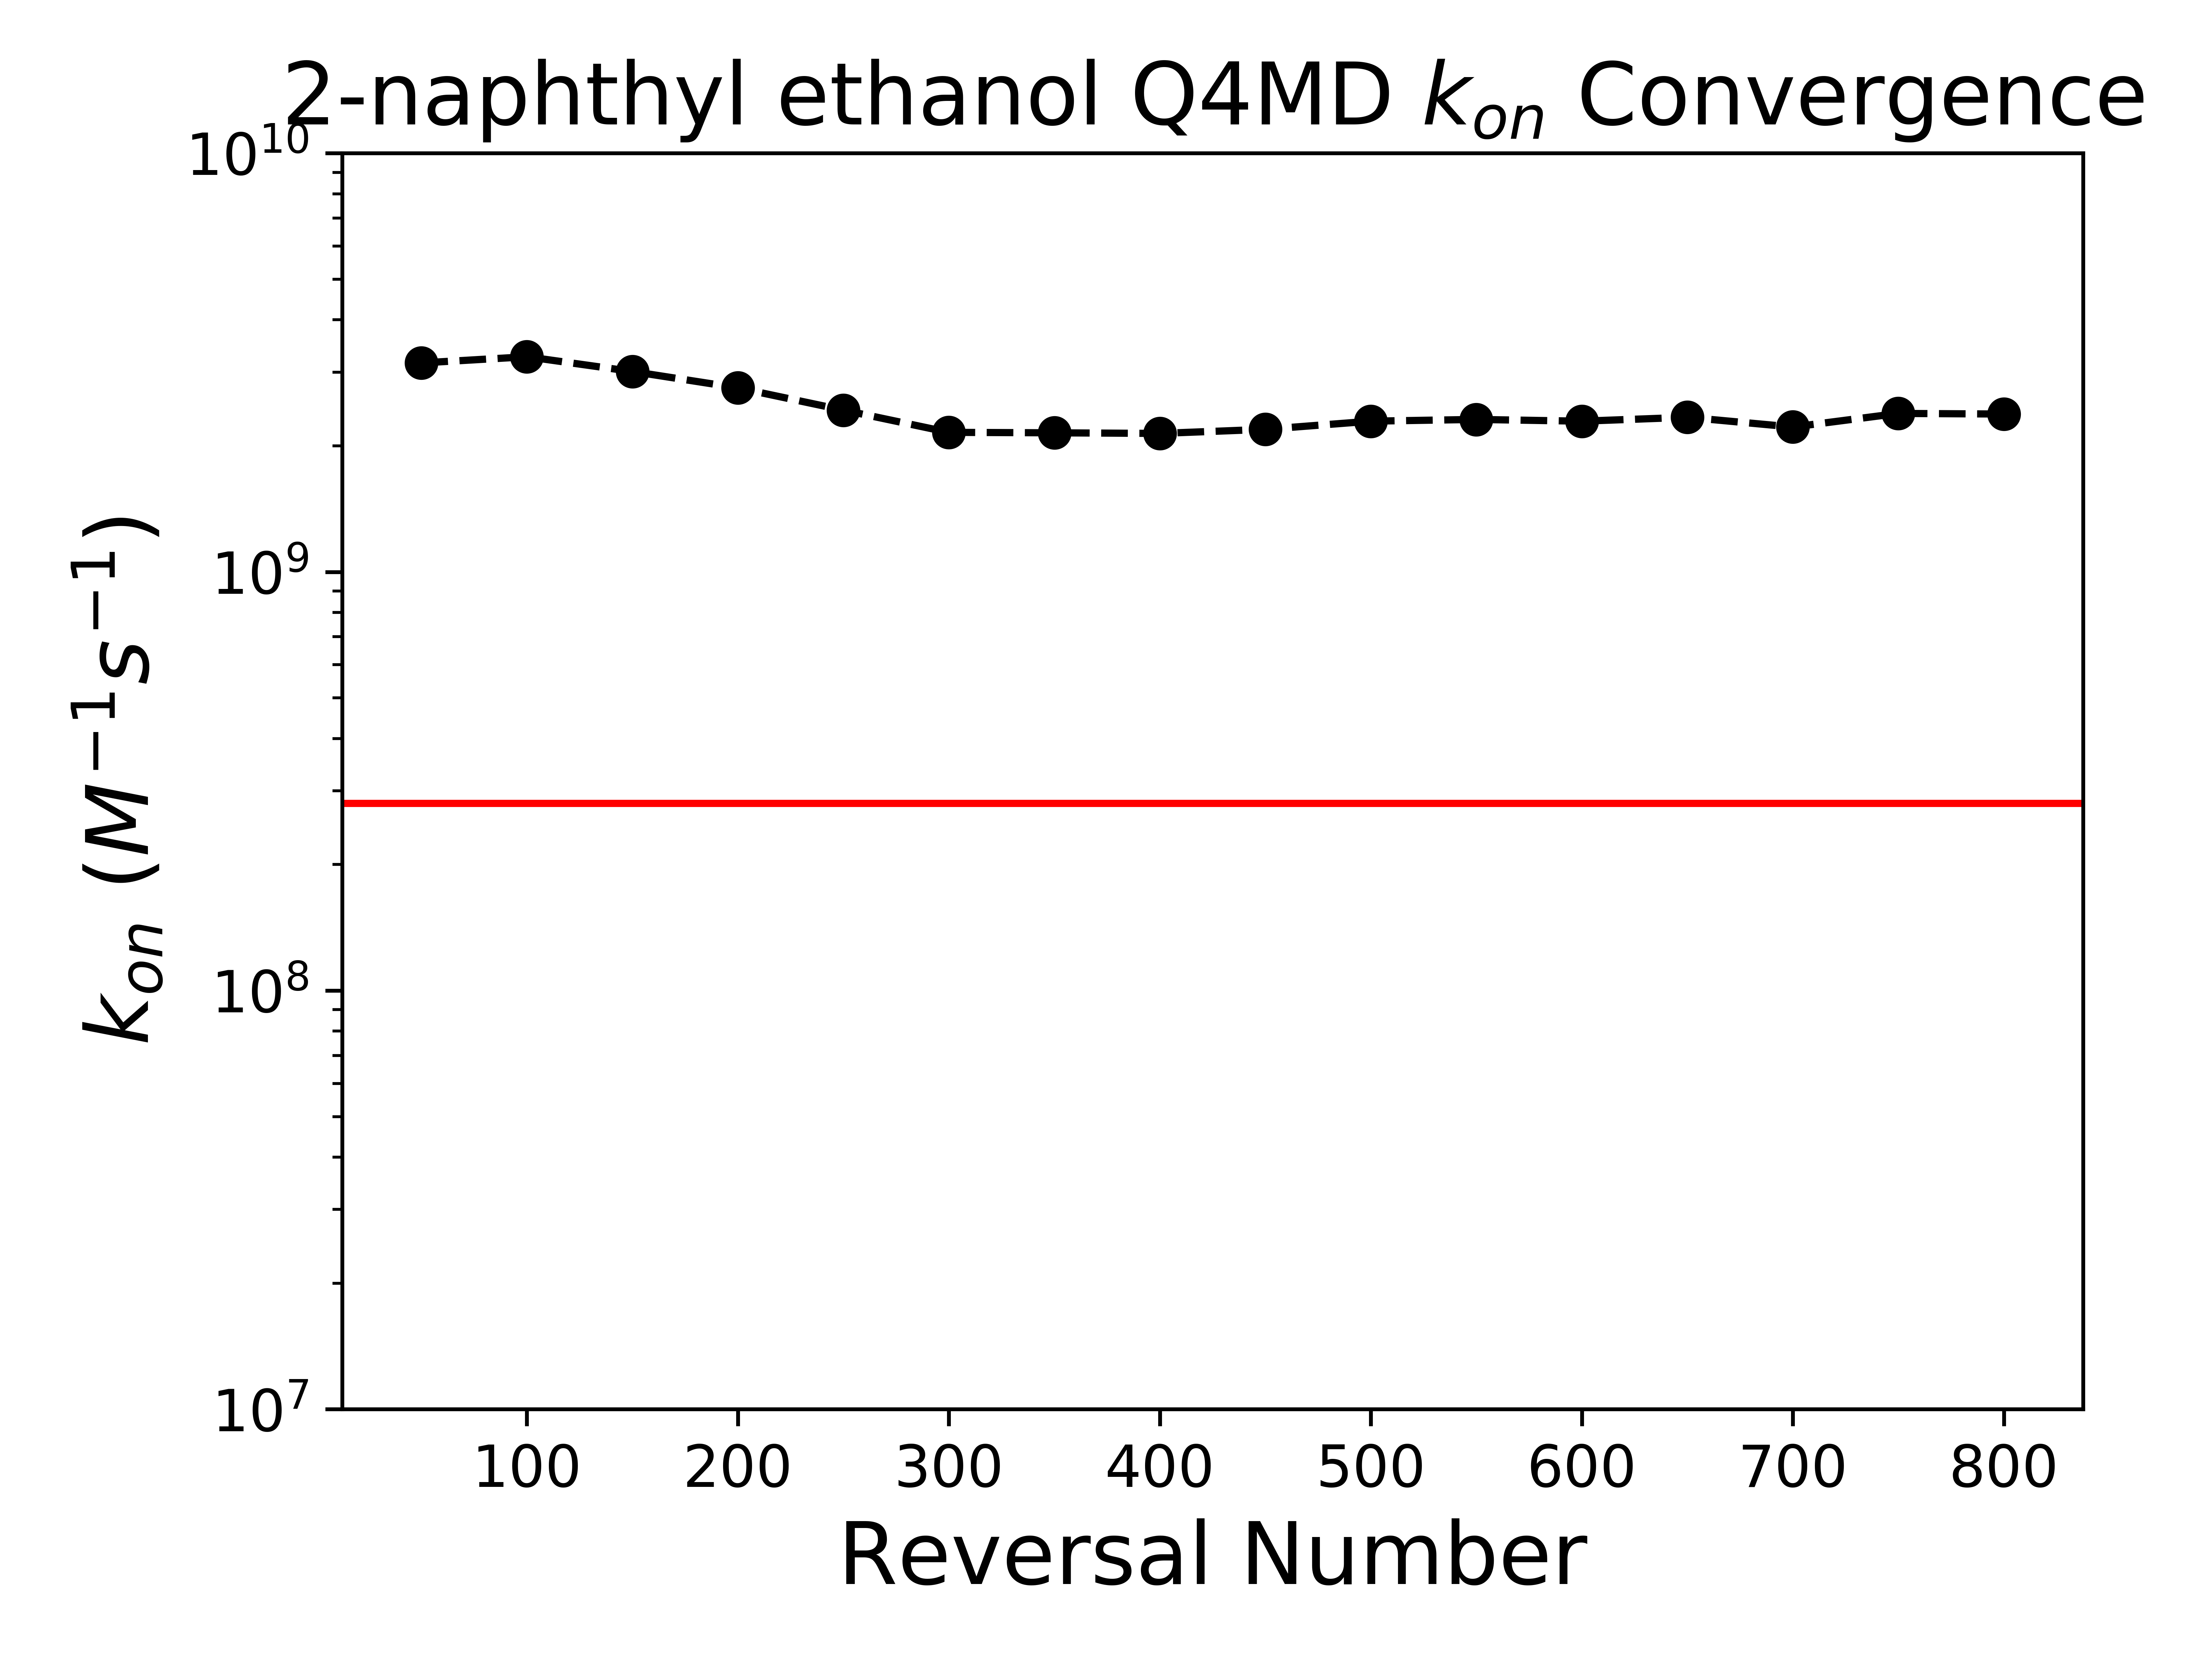
\includegraphics[width=\linewidth]{high_res_images/q4md_rate_conv_images/2-naphthylethanol_q4md_on_conv.png}
\end{subfigure}%
	\begin{subfigure}{0.3\linewidth}
		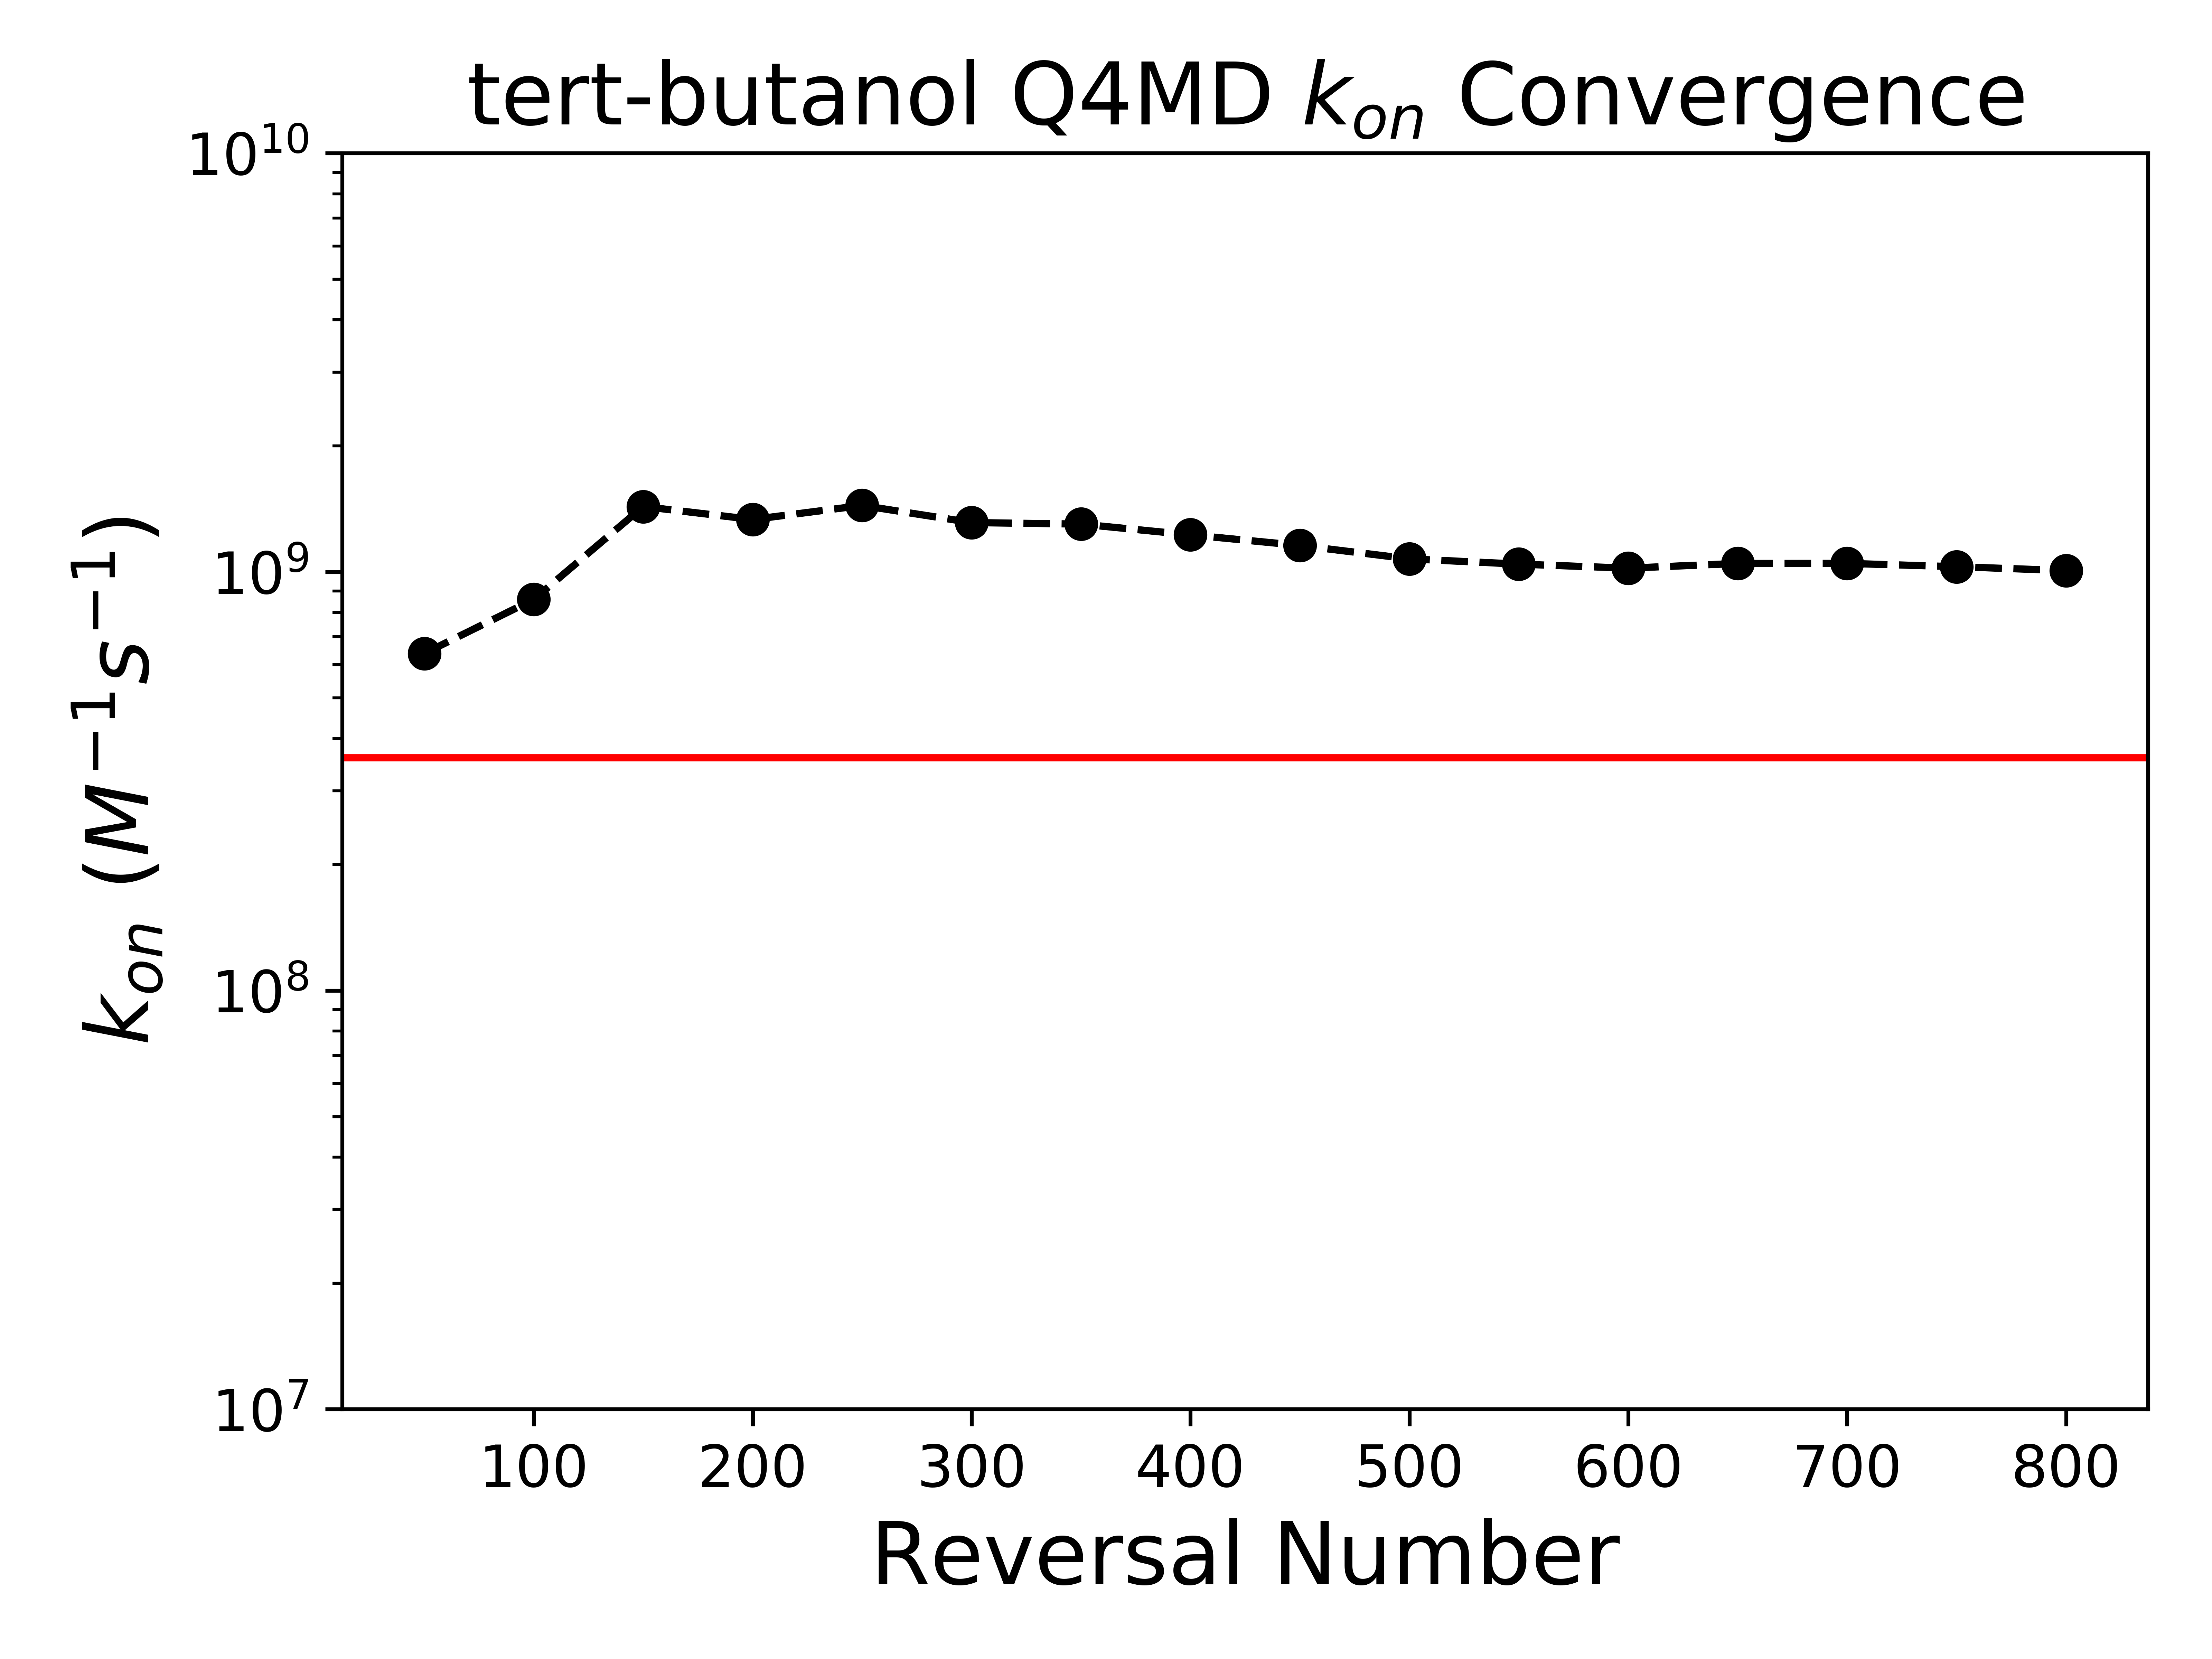
\includegraphics[width=\linewidth]{high_res_images/q4md_rate_conv_images/tert-butanol_q4md_on_conv.png}
	\end{subfigure}
	\begin{subfigure}{0.3\linewidth}
		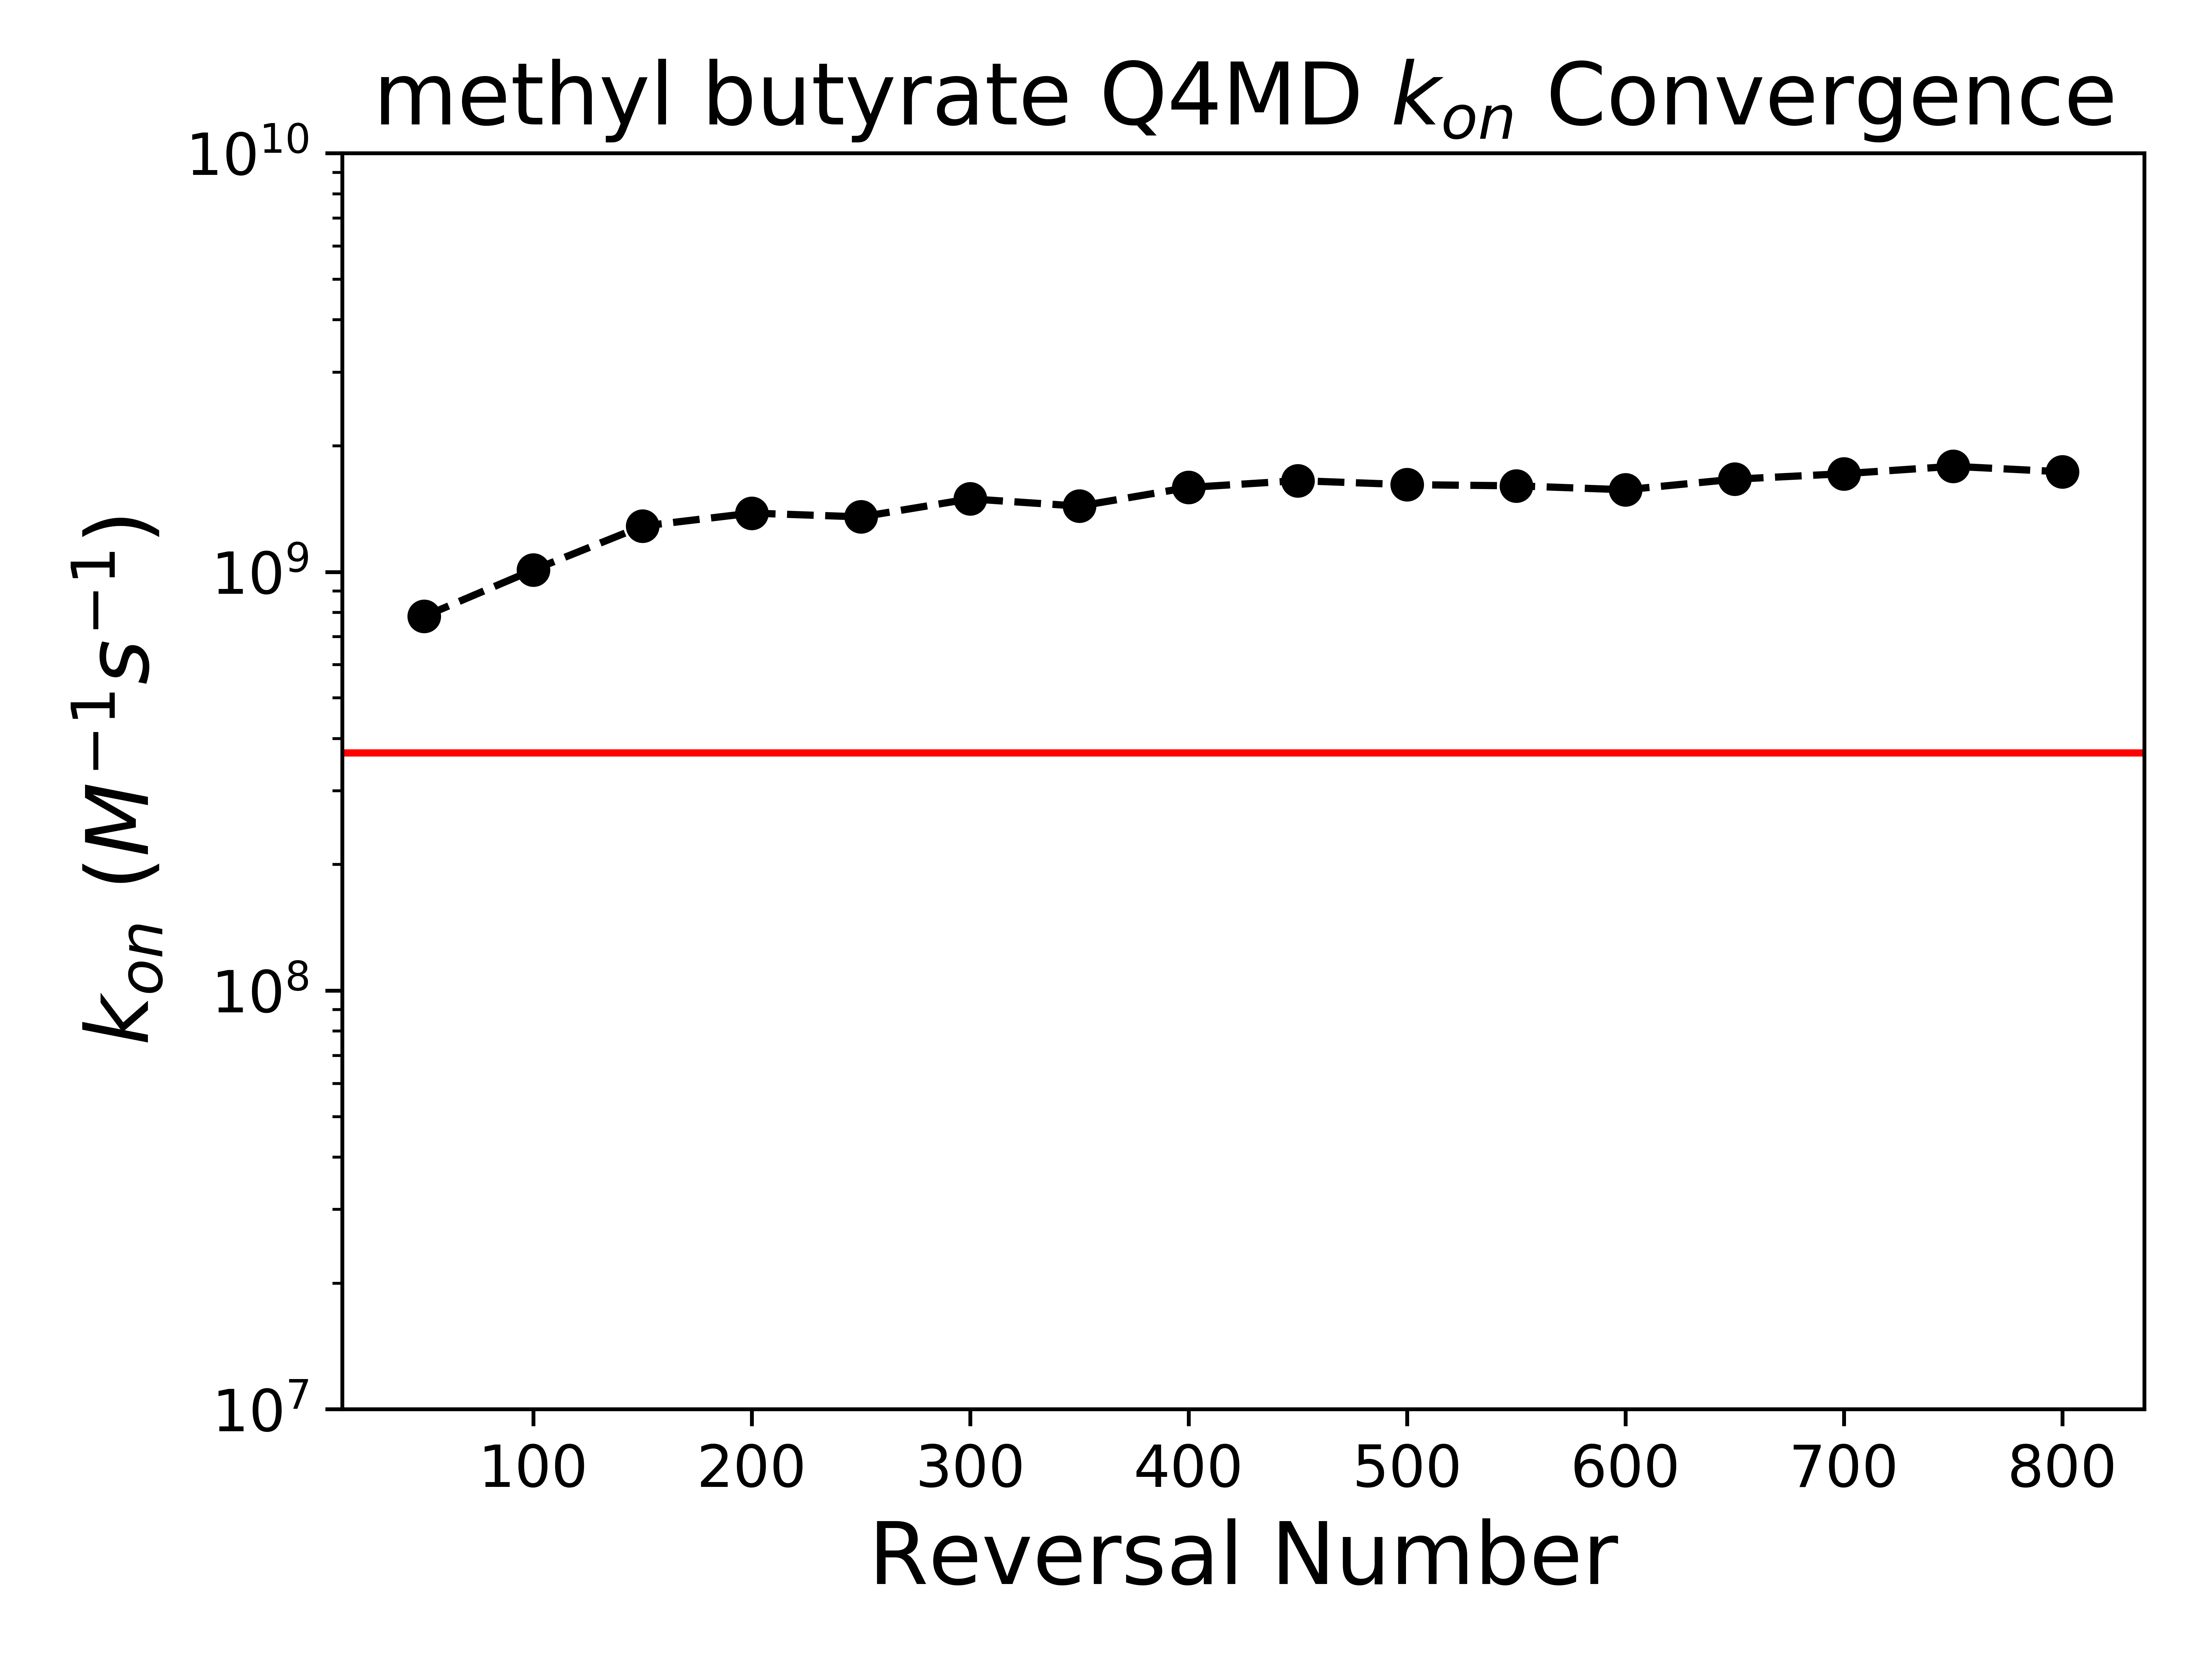
\includegraphics[width=\linewidth]{high_res_images/q4md_rate_conv_images/methylbutyrate_q4md_on_conv.png}
	\end{subfigure}
	\begin{subfigure}{0.3\linewidth}
		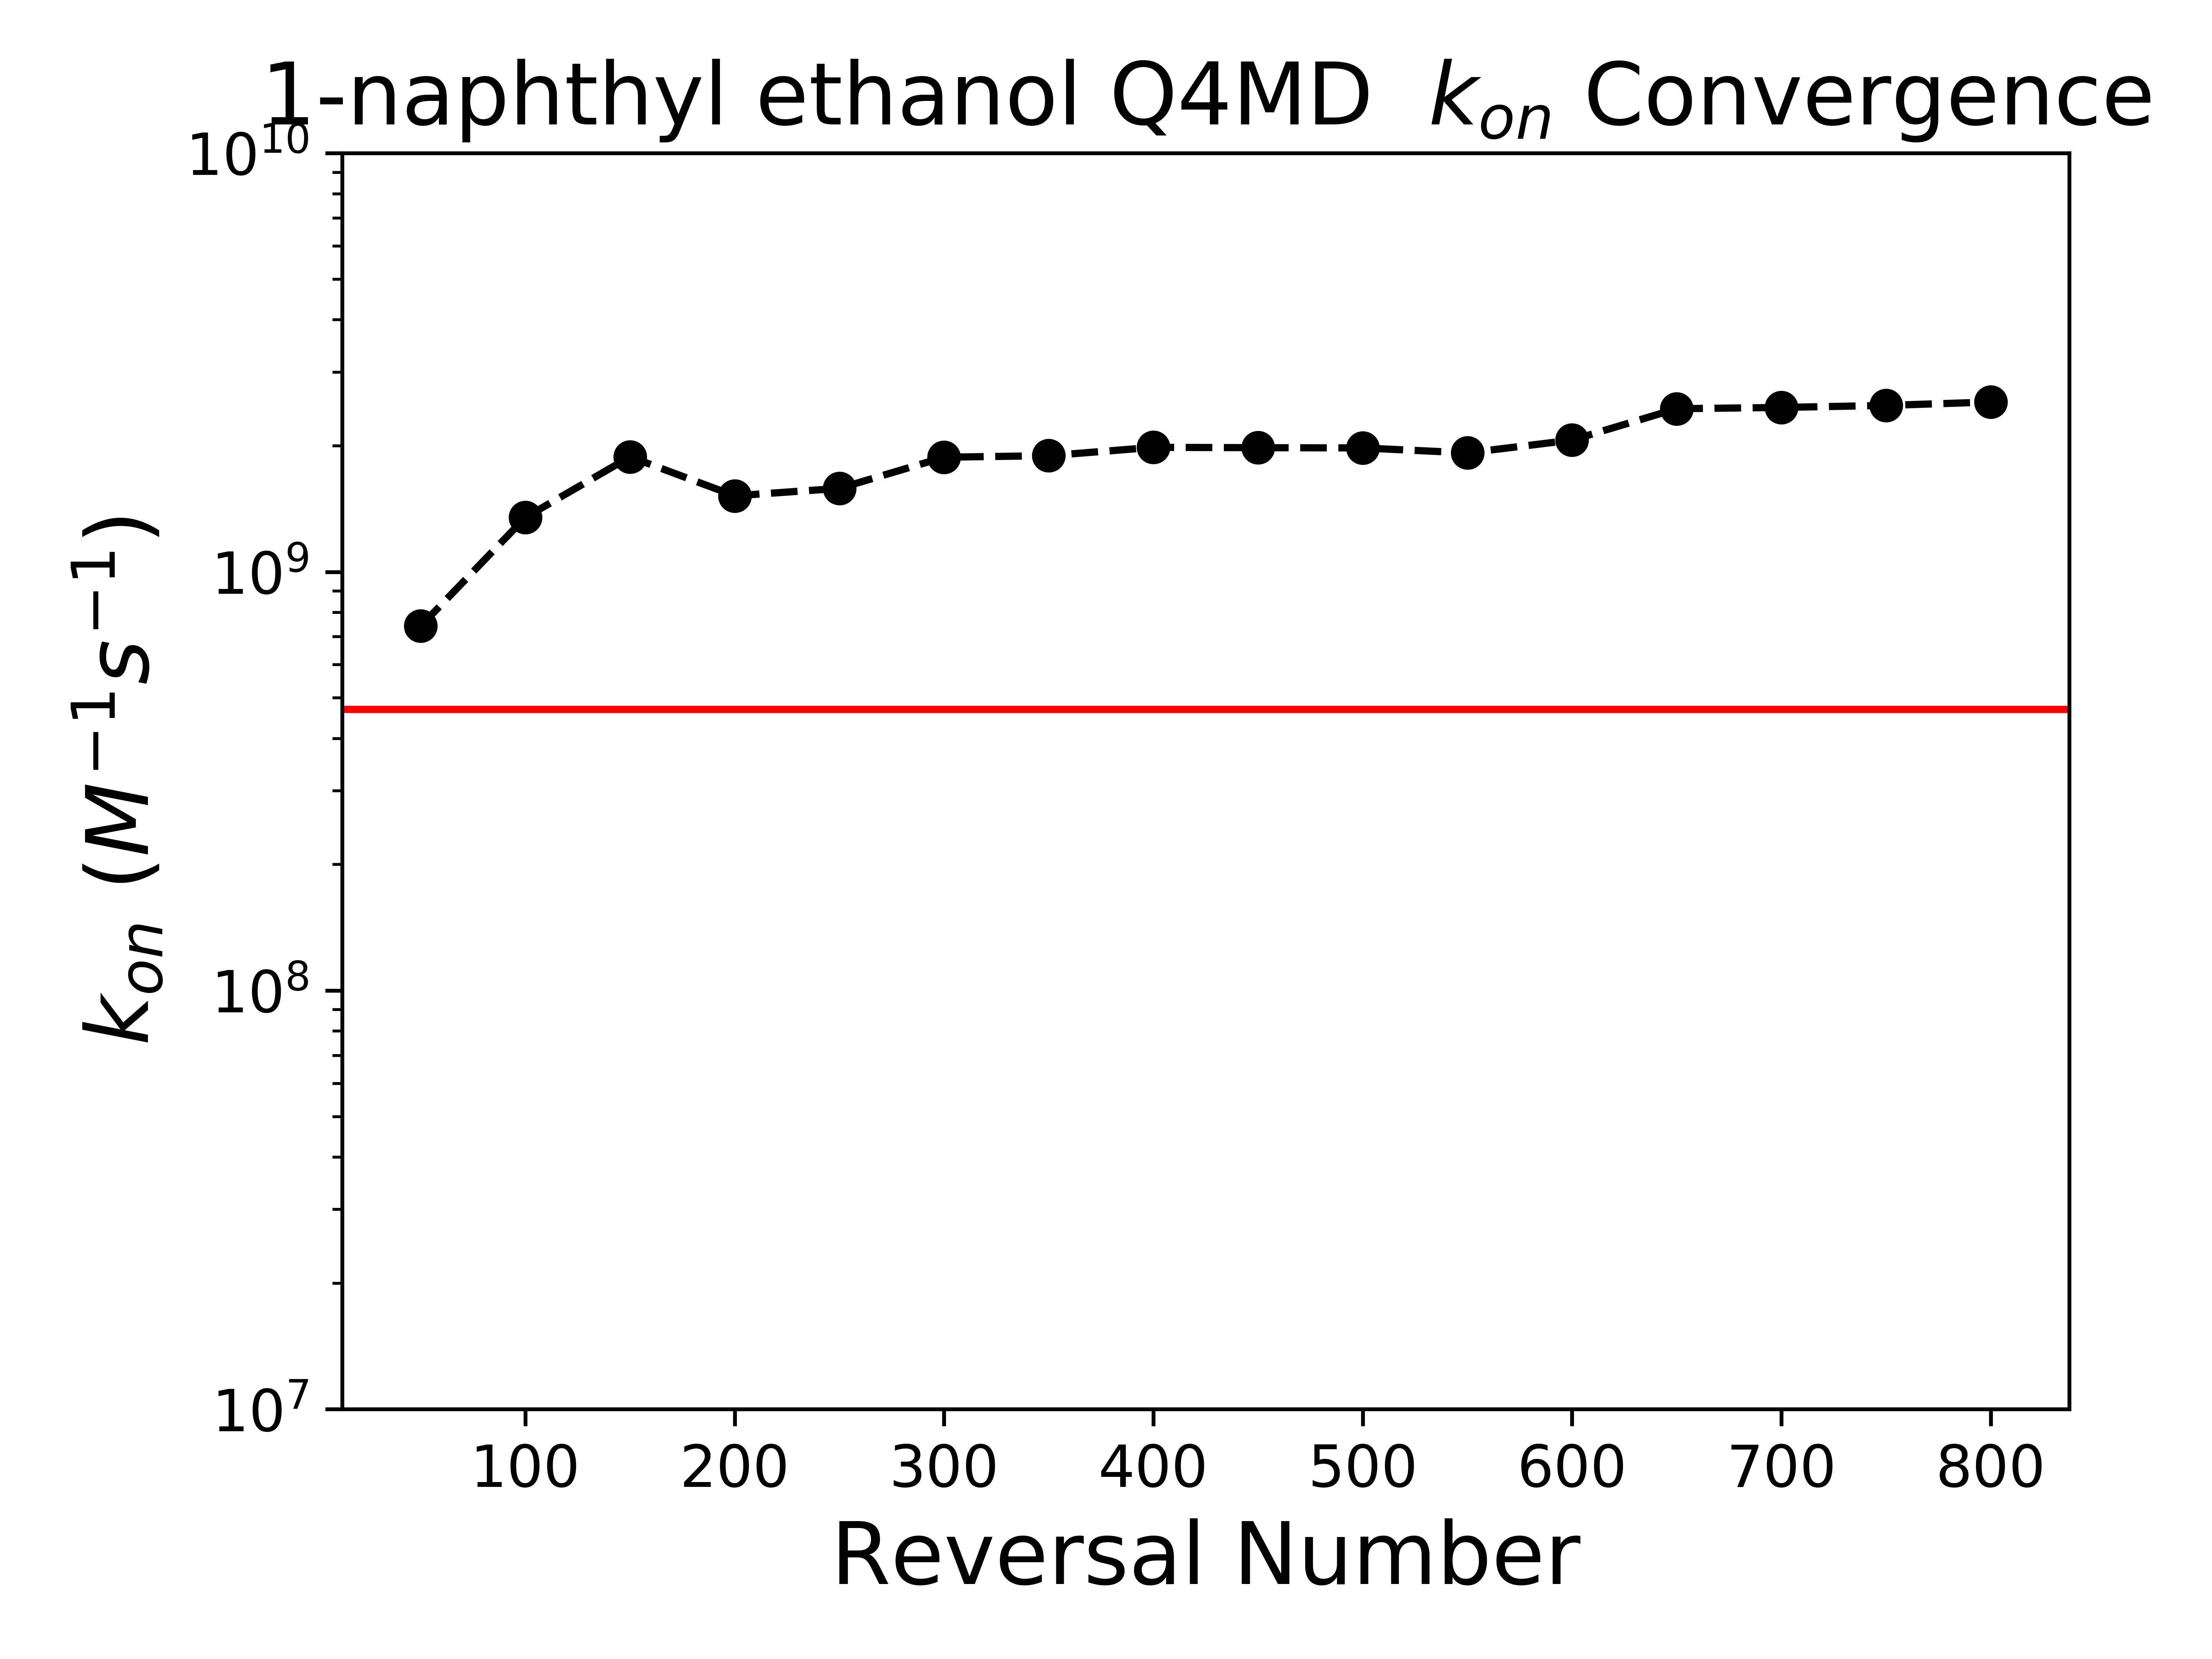
\includegraphics[width=\linewidth]{high_res_images/q4md_rate_conv_images/1-naphthylethanol_q4md_on_conv.png}
	\end{subfigure}
	\begin{subfigure}{0.3\linewidth}
		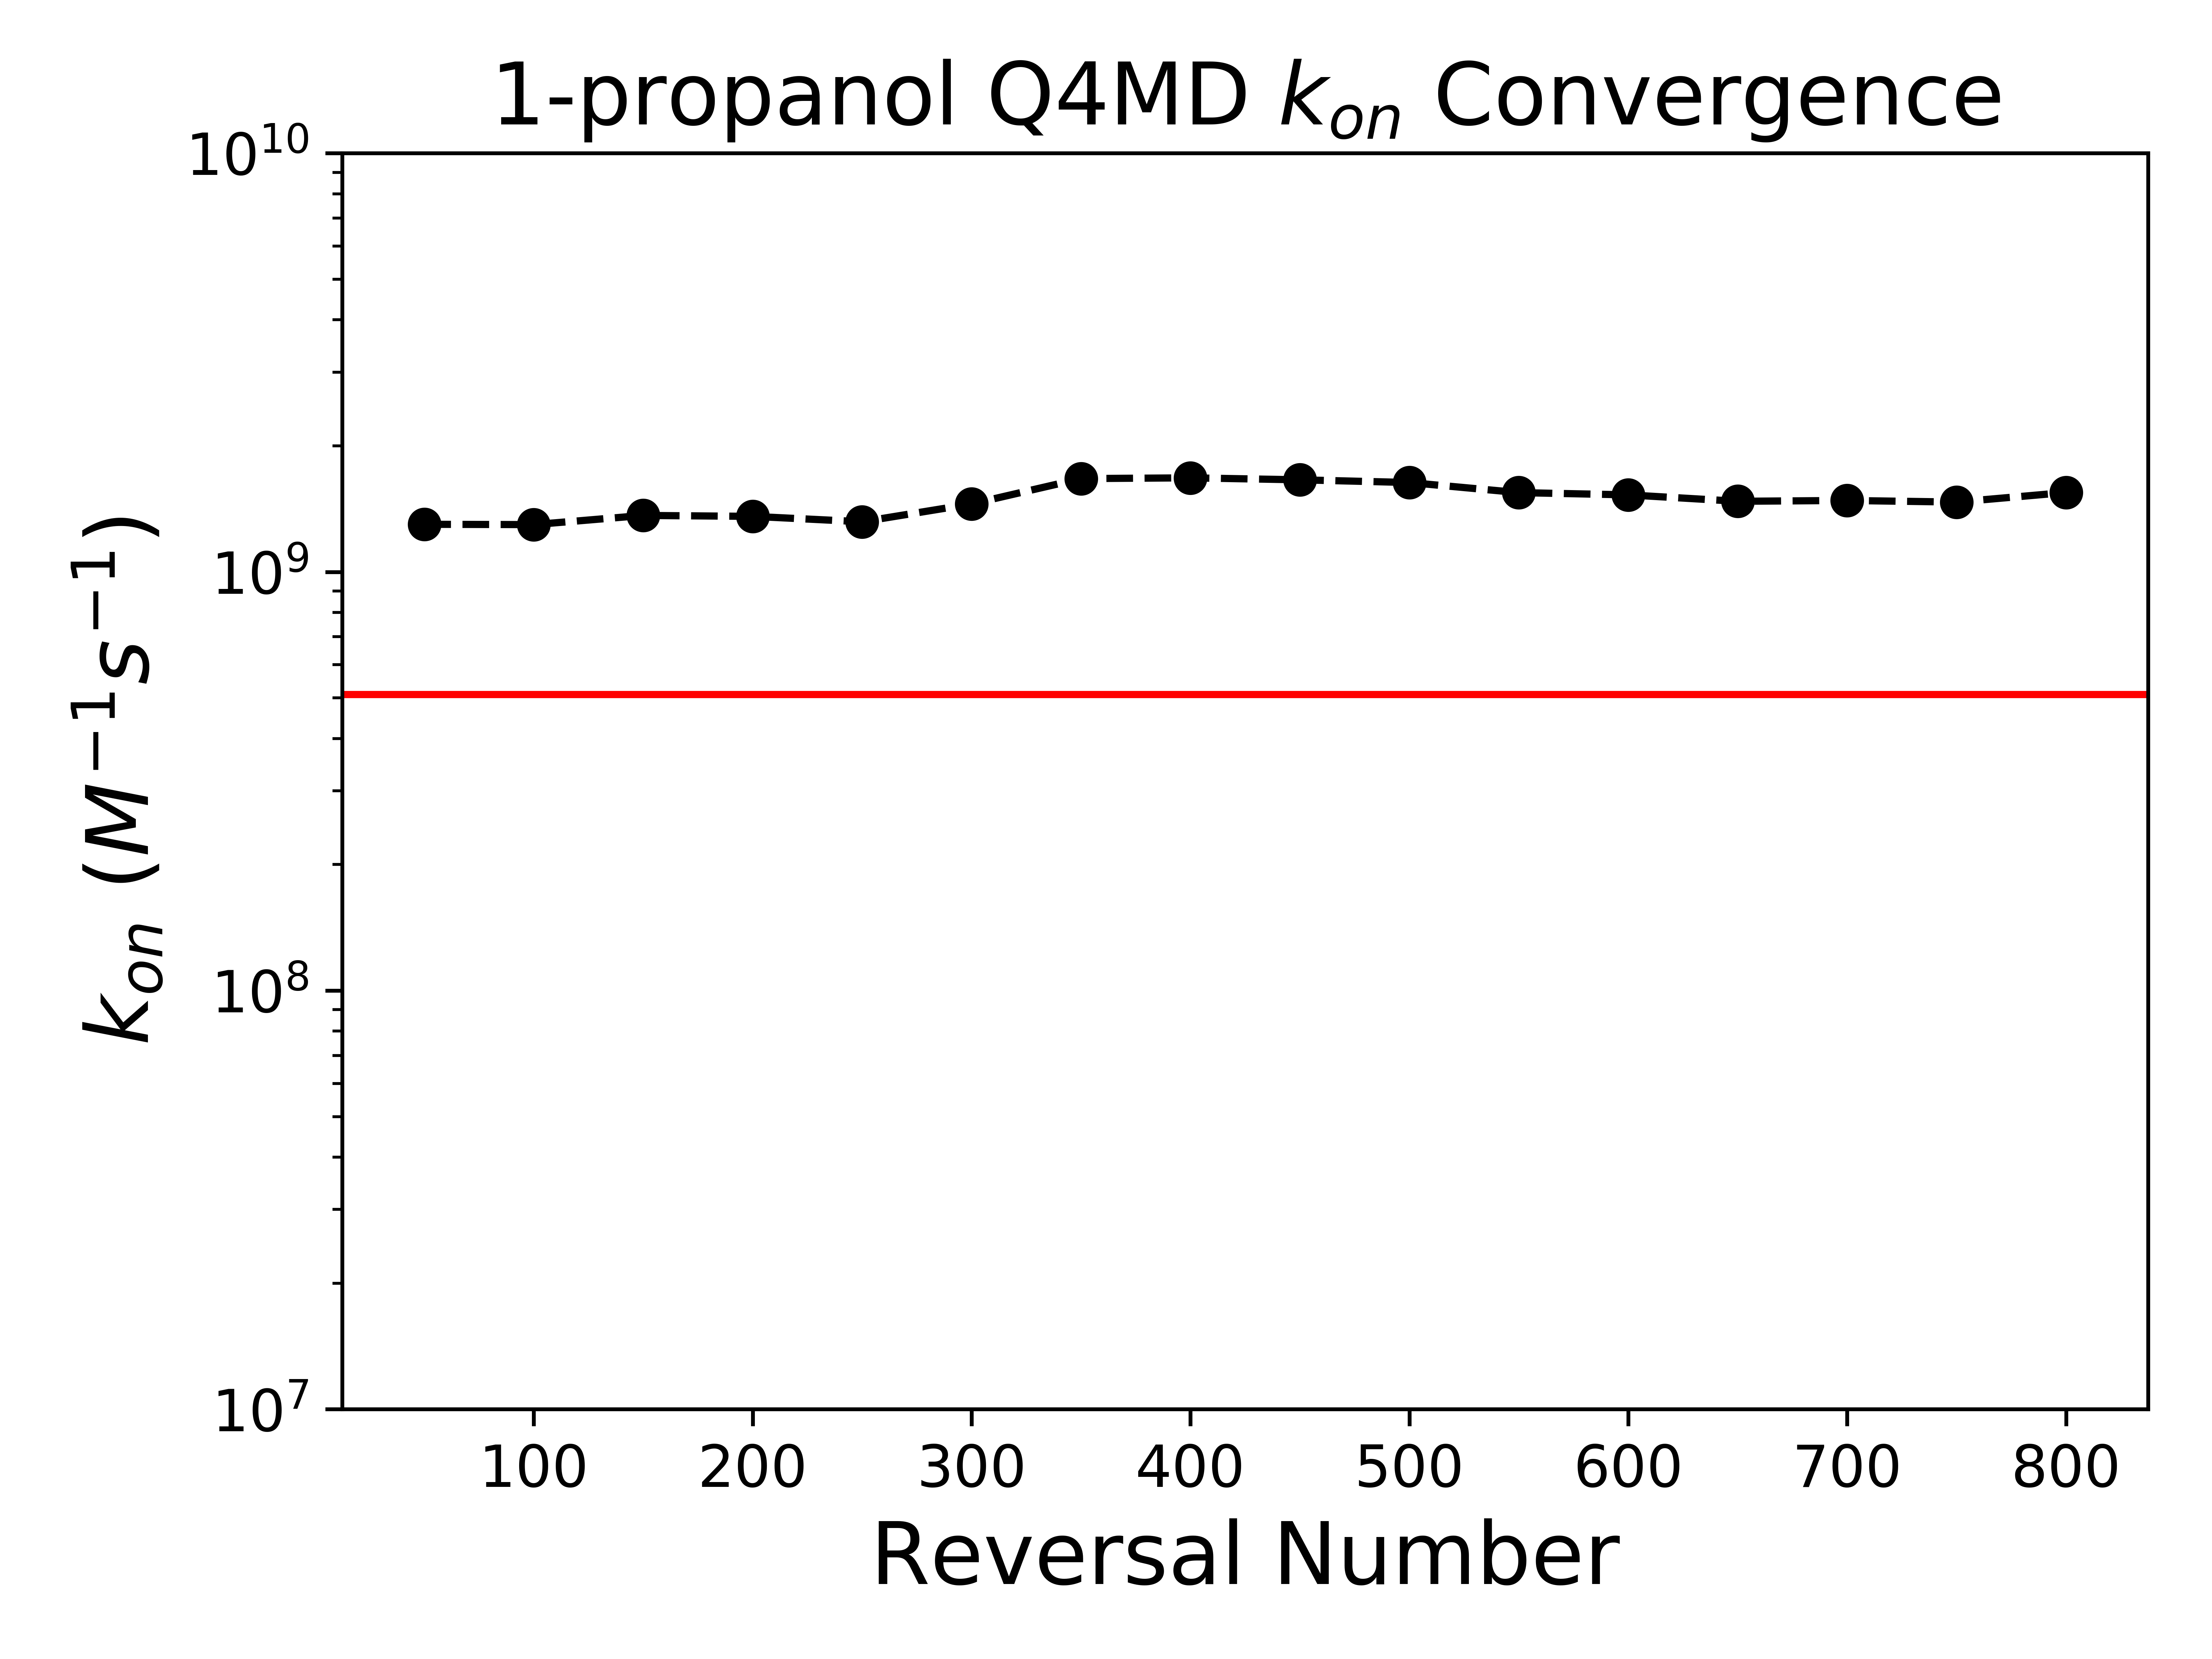
\includegraphics[width=\linewidth]{high_res_images/q4md_rate_conv_images/1-propanol_q4md_on_conv.png}
	\end{subfigure}
	\begin{subfigure}{0.3\linewidth}
		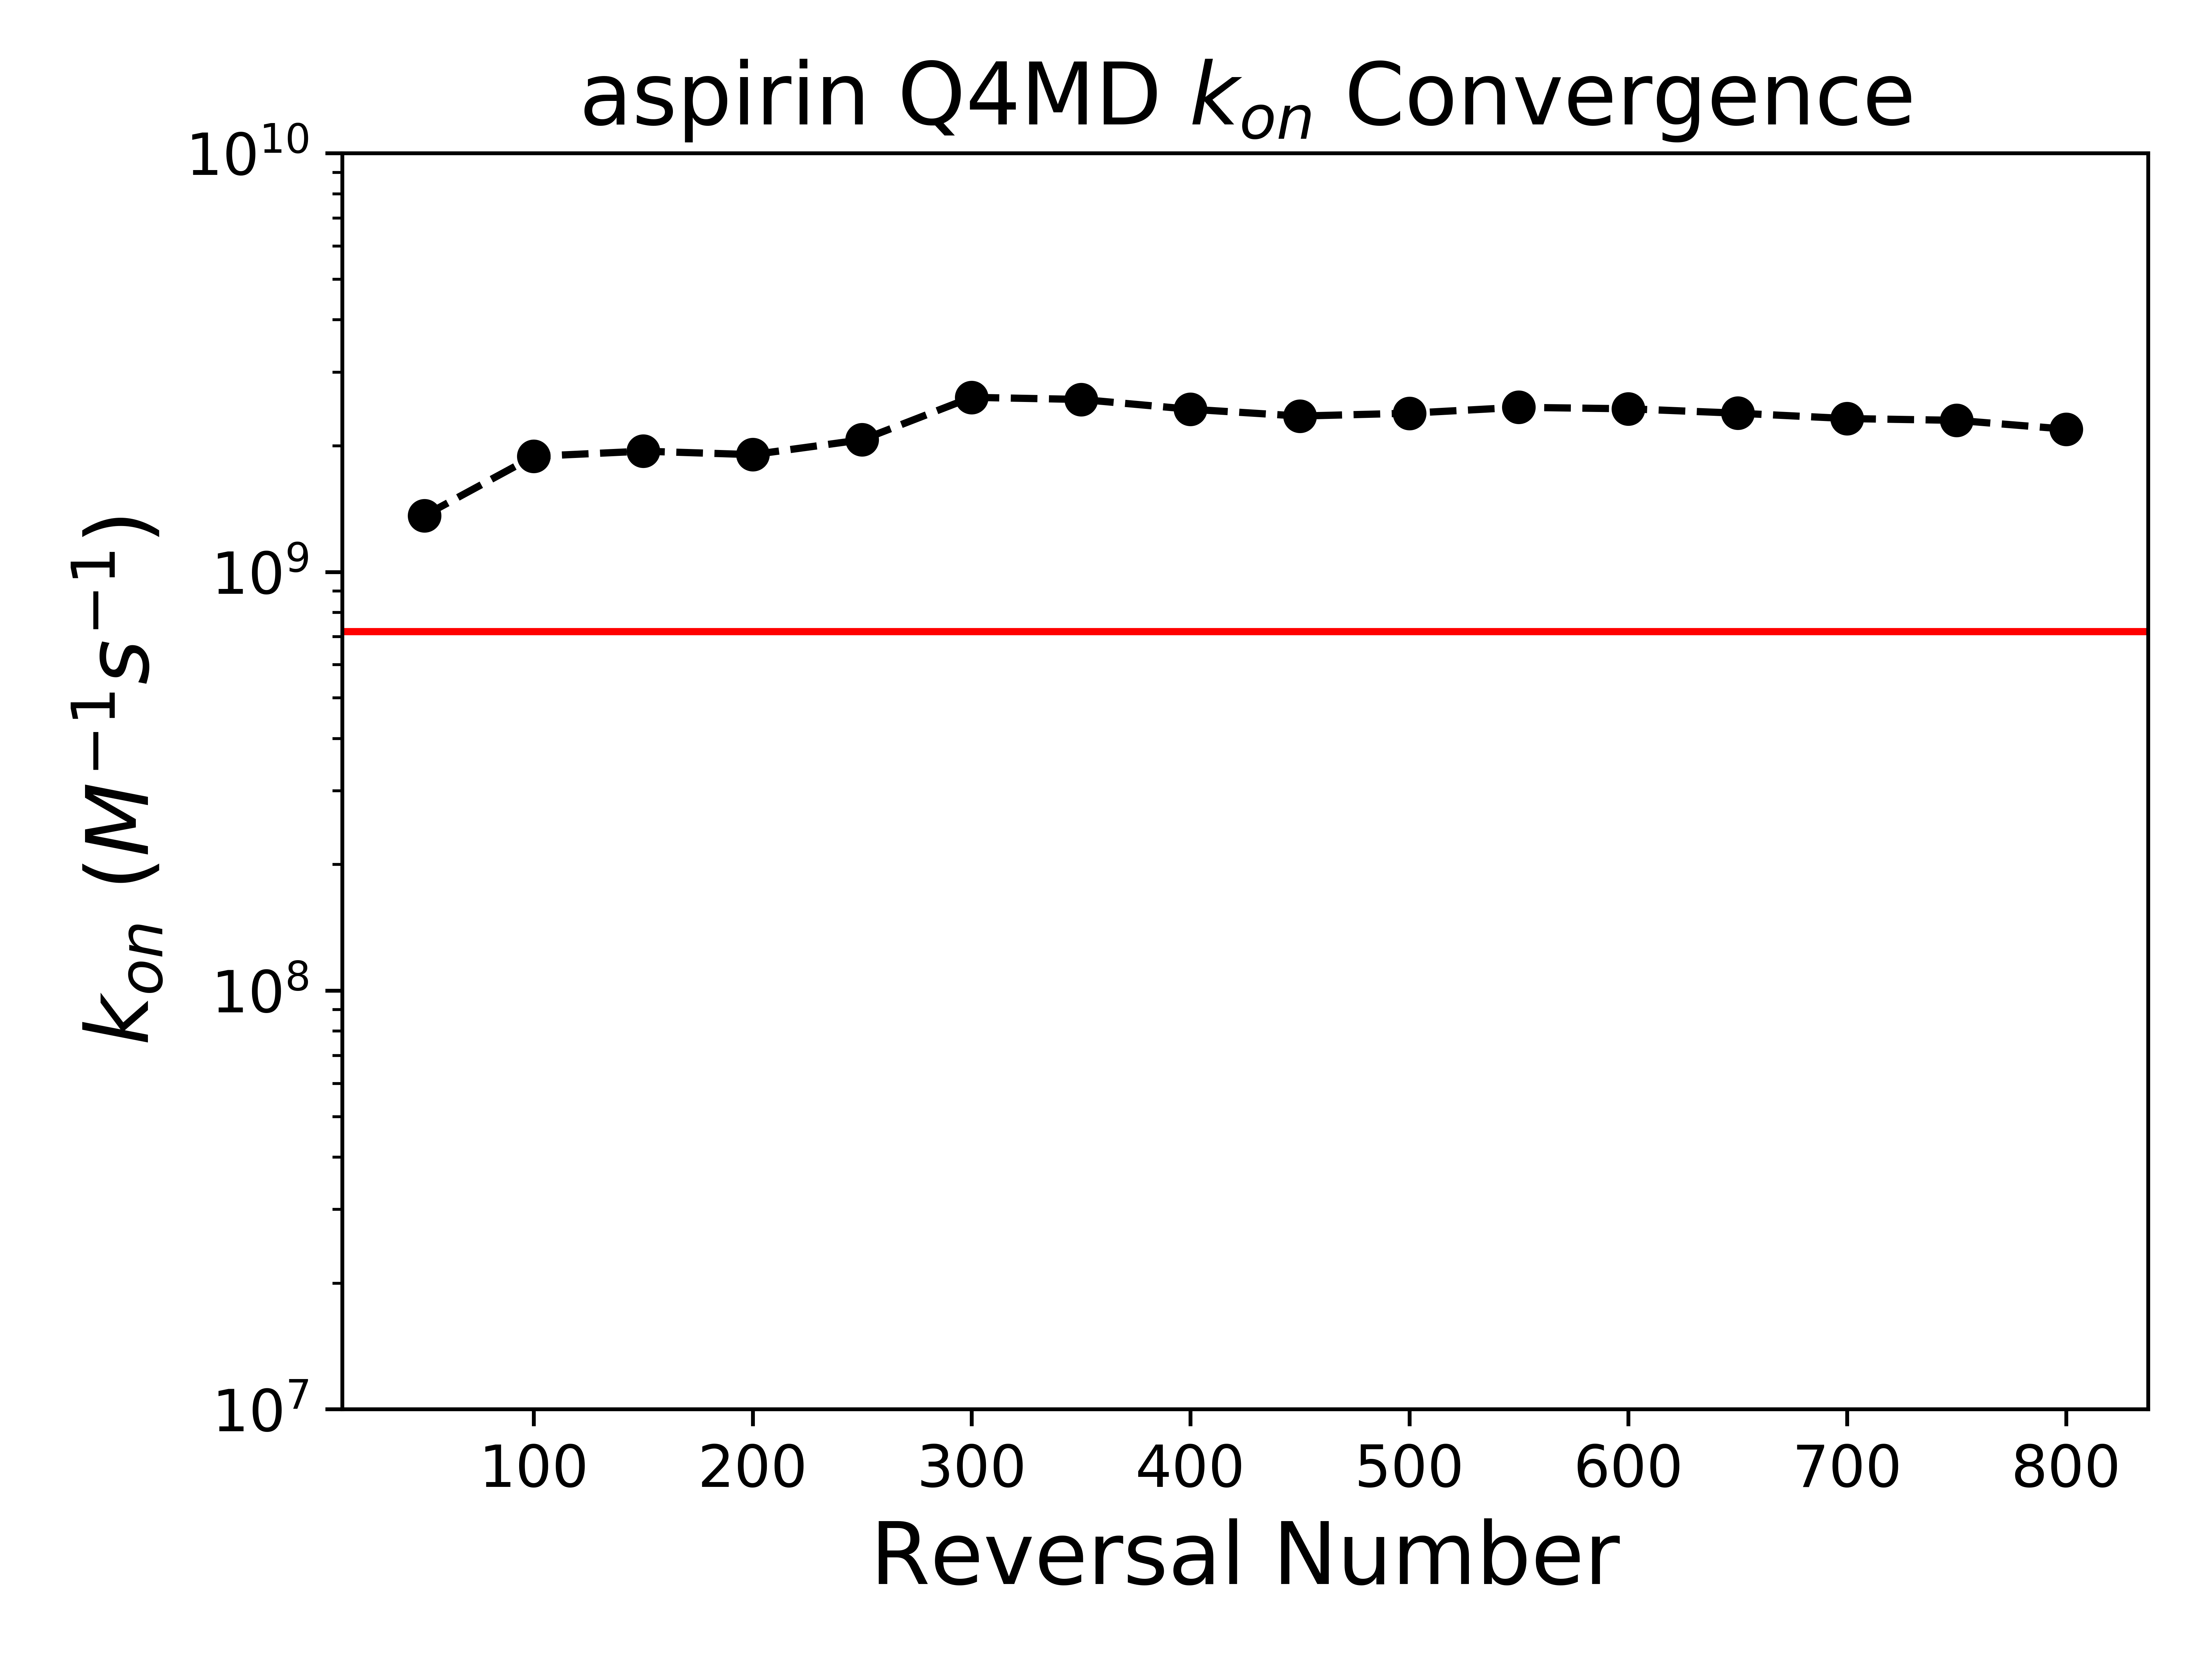
\includegraphics[width=\linewidth]{high_res_images/q4md_rate_conv_images/aspirin_q4md_on_conv.png}
	\end{subfigure}
	\caption{Convergence of on rates as a function of the number of reversals included using the Q4MD forcefield}
\end{figure}
%\begin{figure}
\begin{subfigure}{0.3\linewidth}
	\centering
	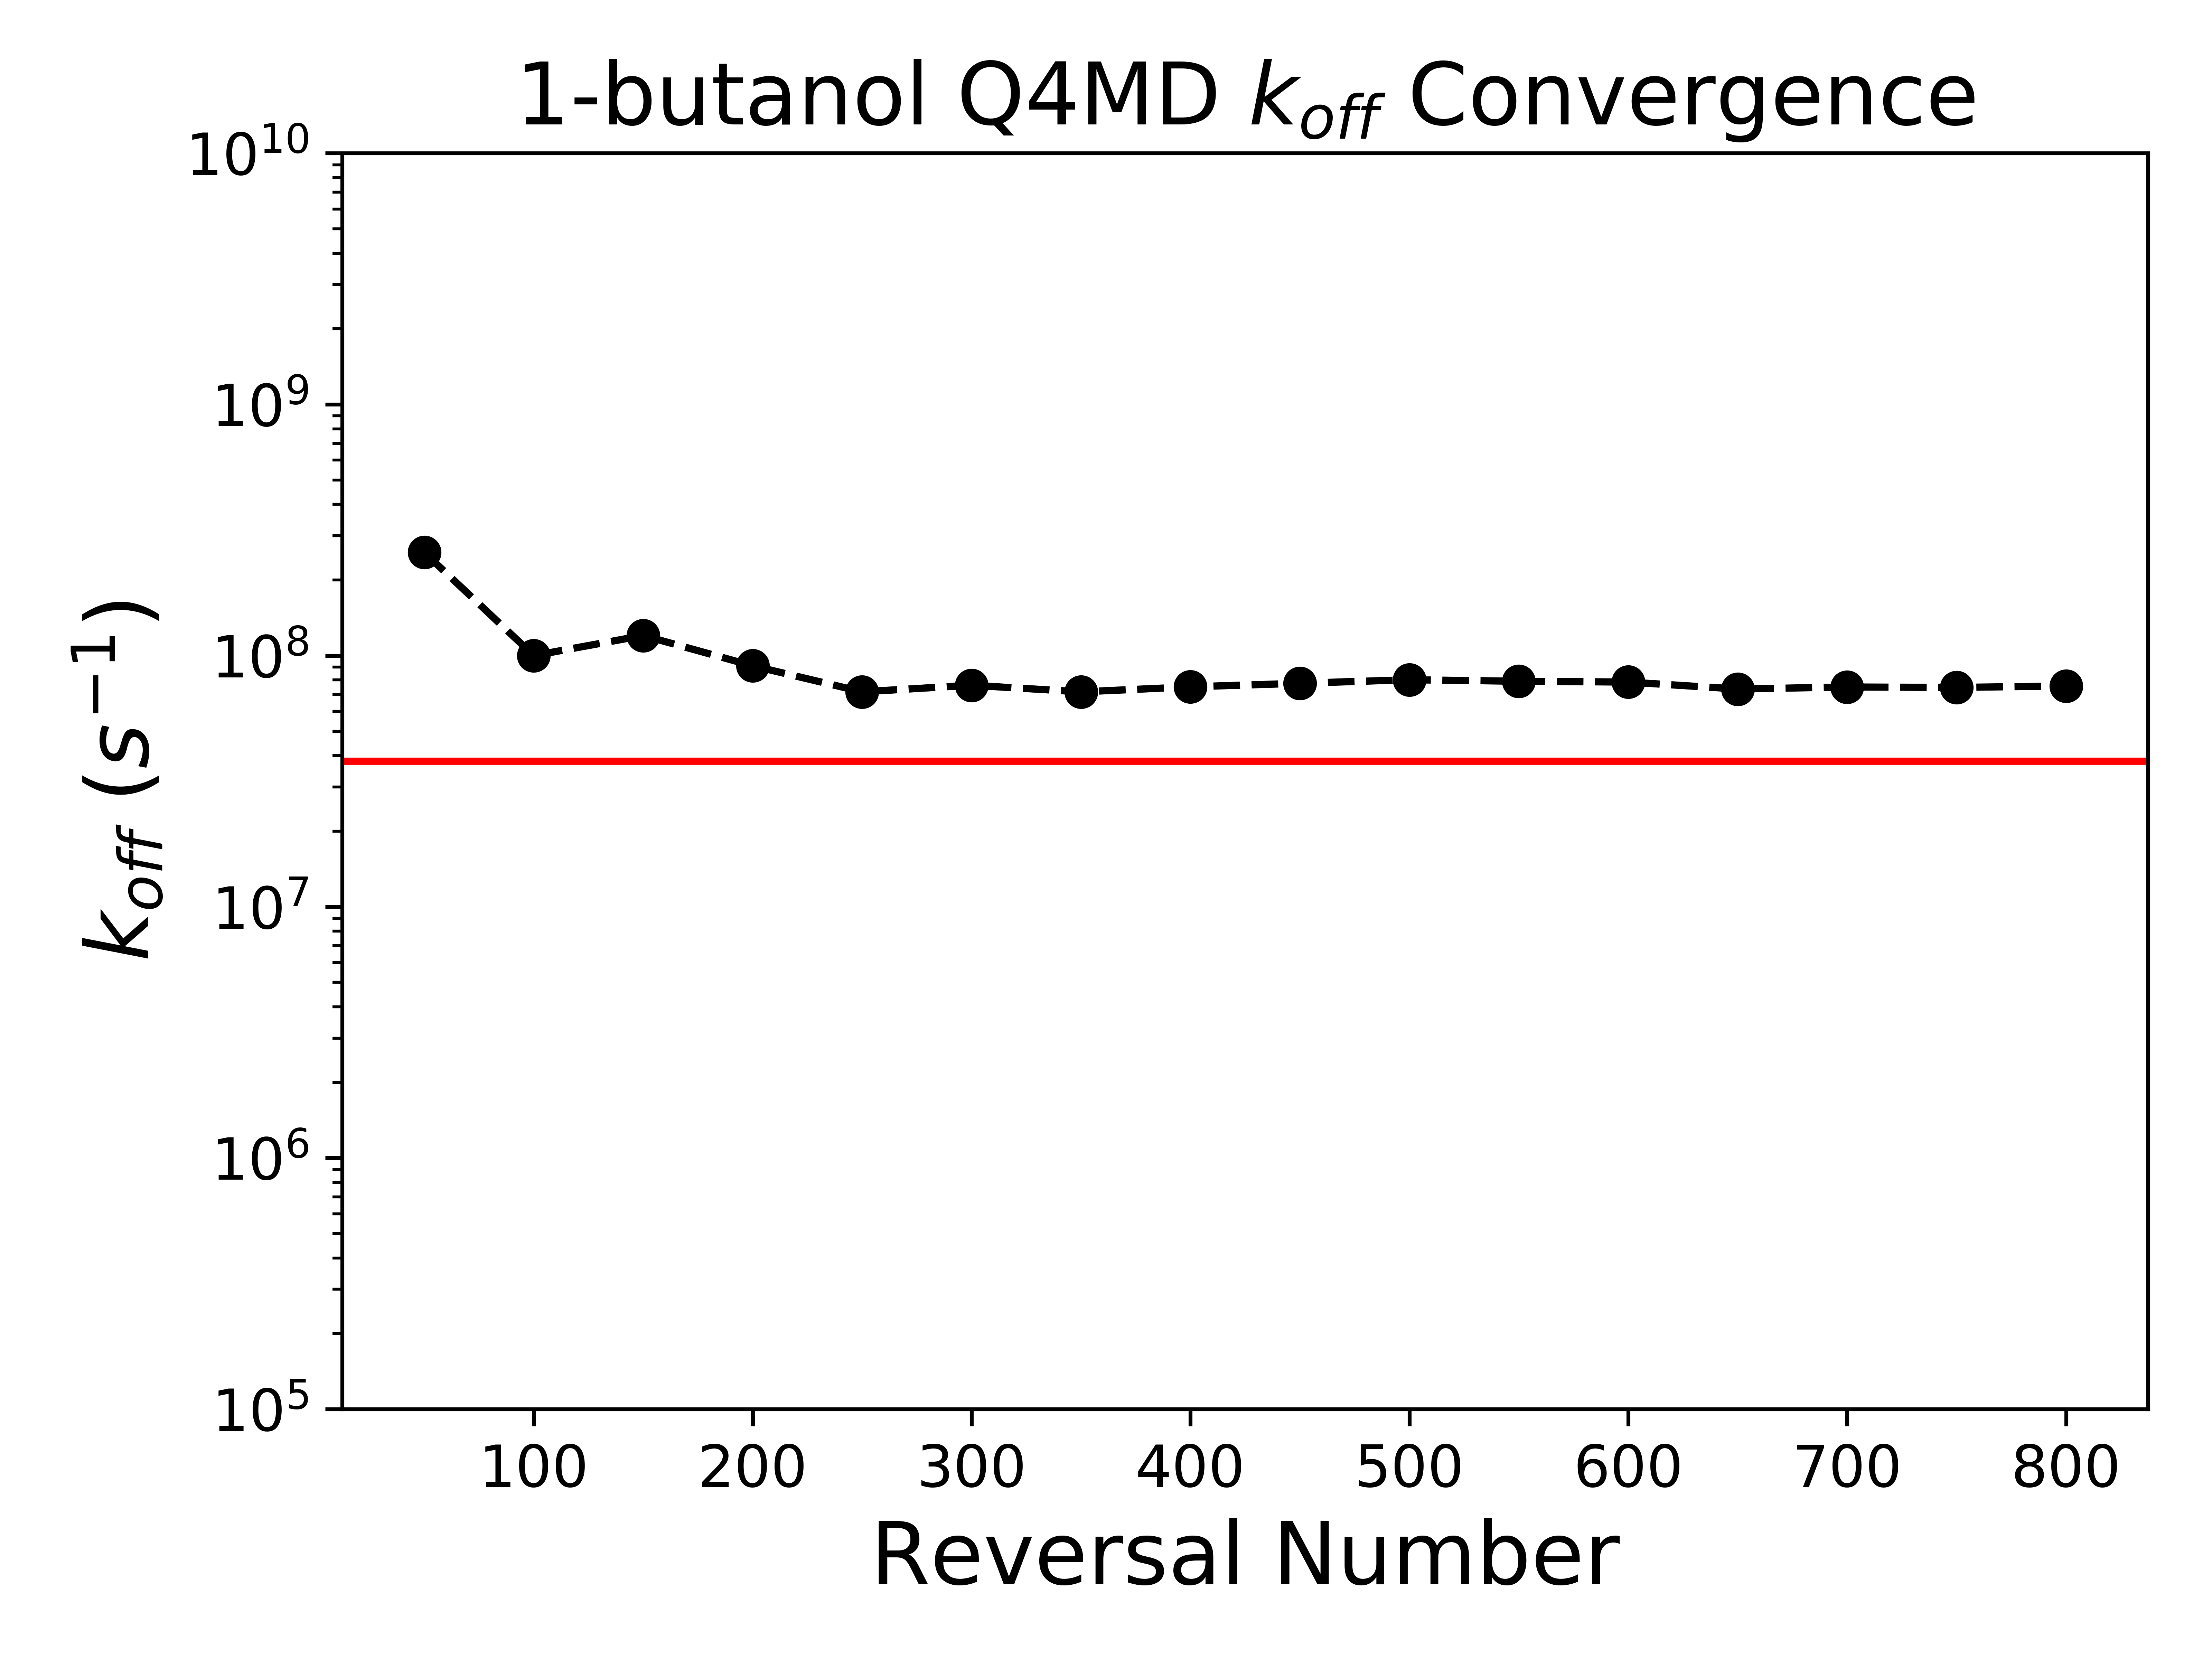
\includegraphics[width=\linewidth]{high_res_images/q4md_rate_conv_images/1-butanol_q4md_off_conv.png}
	\end{subfigure}%
\begin{subfigure}{0.3\linewidth}
		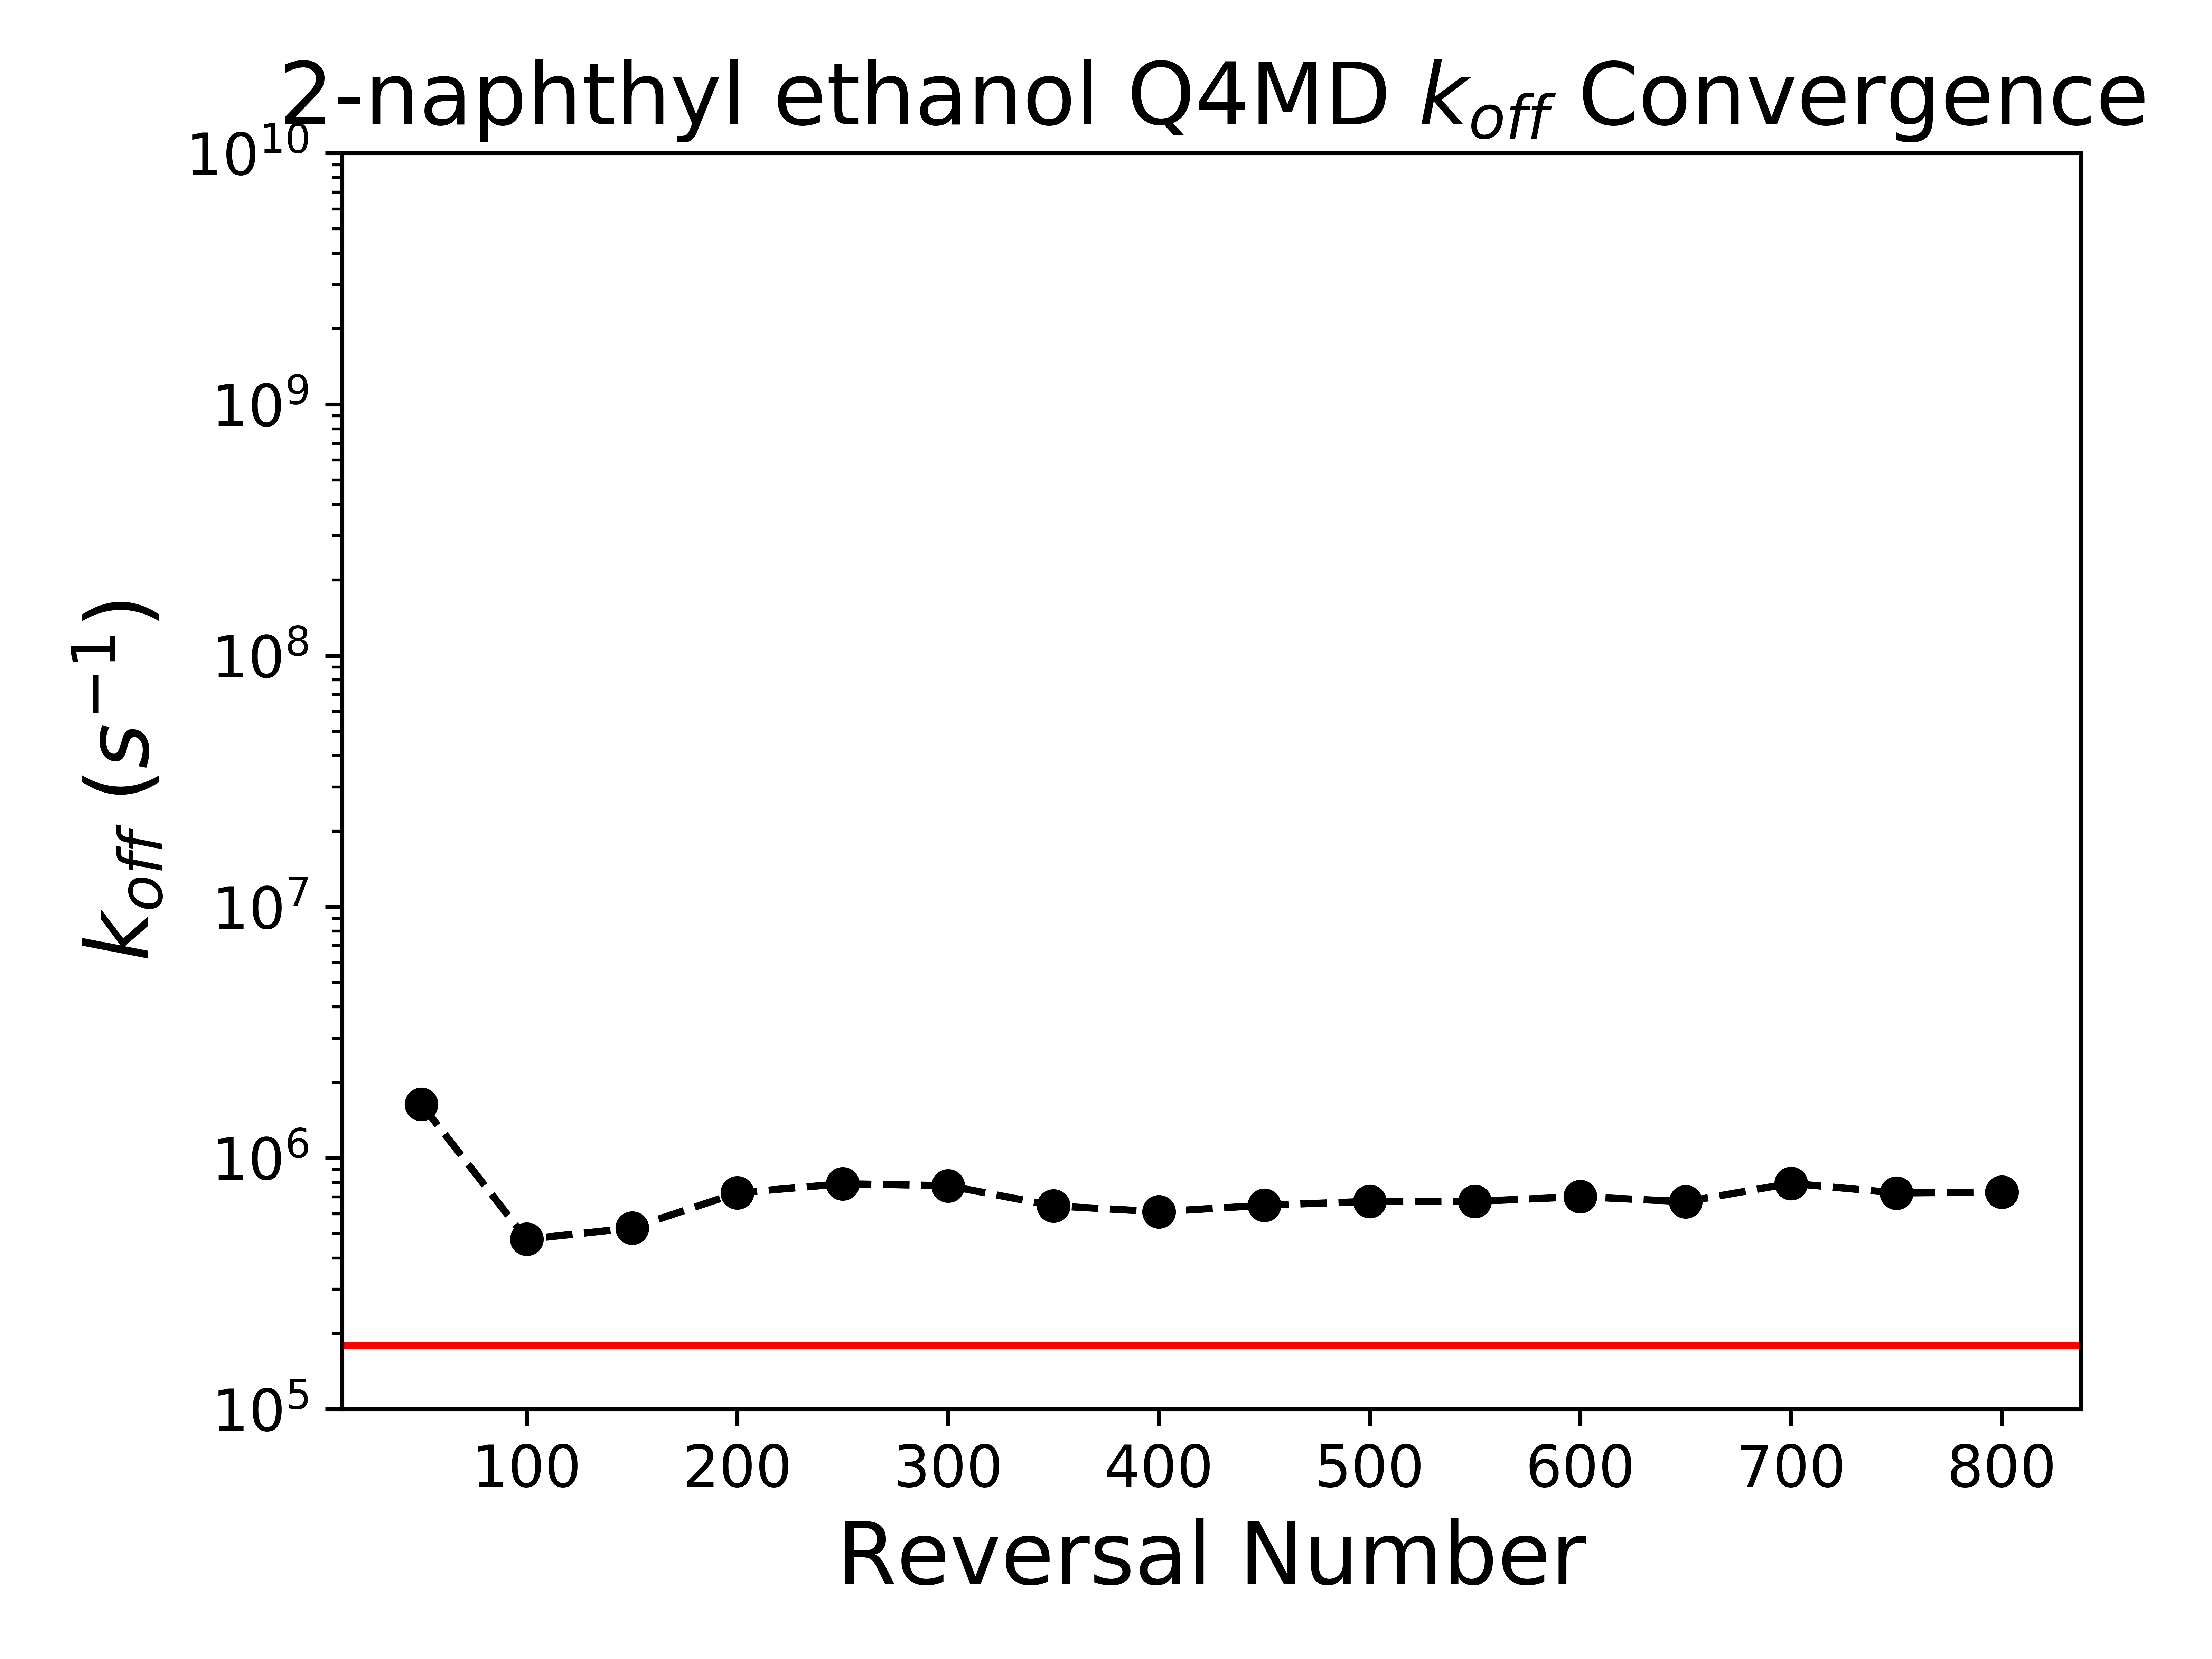
\includegraphics[width=\linewidth]{high_res_images/q4md_rate_conv_images/2-naphthylethanol_q4md_off_conv.png}
\end{subfigure}%
	\begin{subfigure}{0.3\linewidth}
		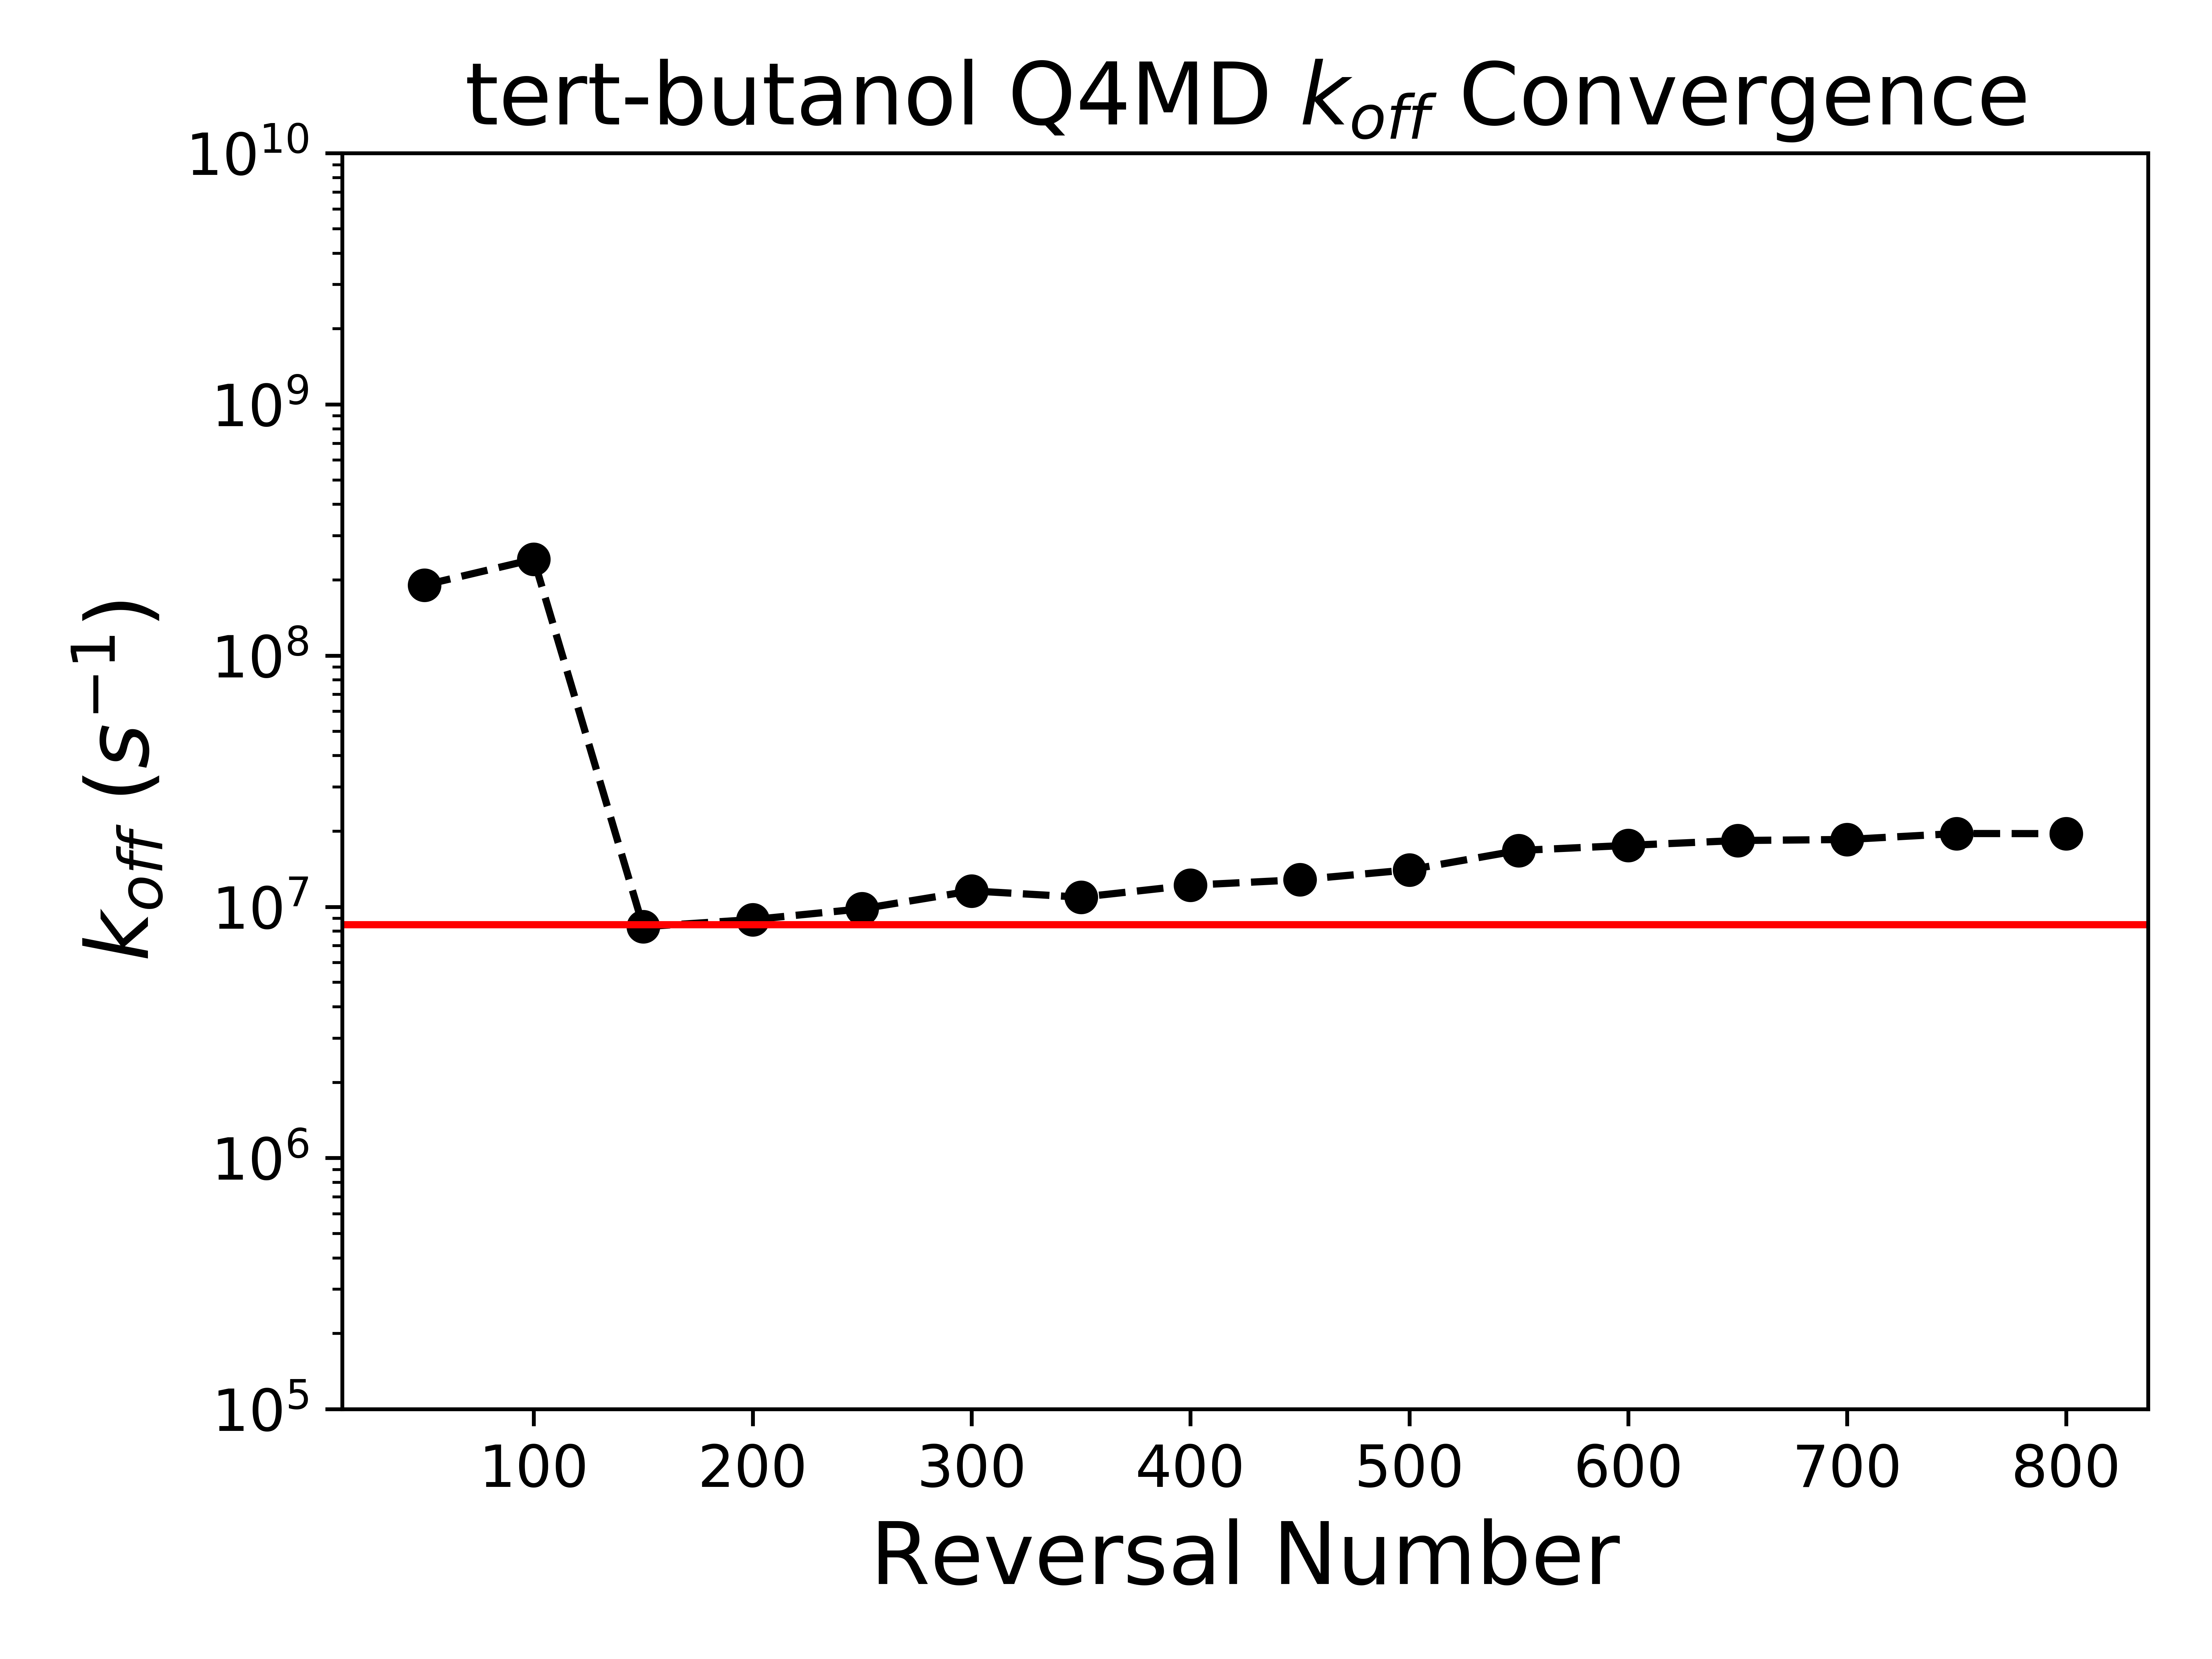
\includegraphics[width=\linewidth]{high_res_images/q4md_rate_conv_images/tert-butanol_q4md_off_conv.png}
	\end{subfigure}
	\begin{subfigure}{0.3\linewidth}
		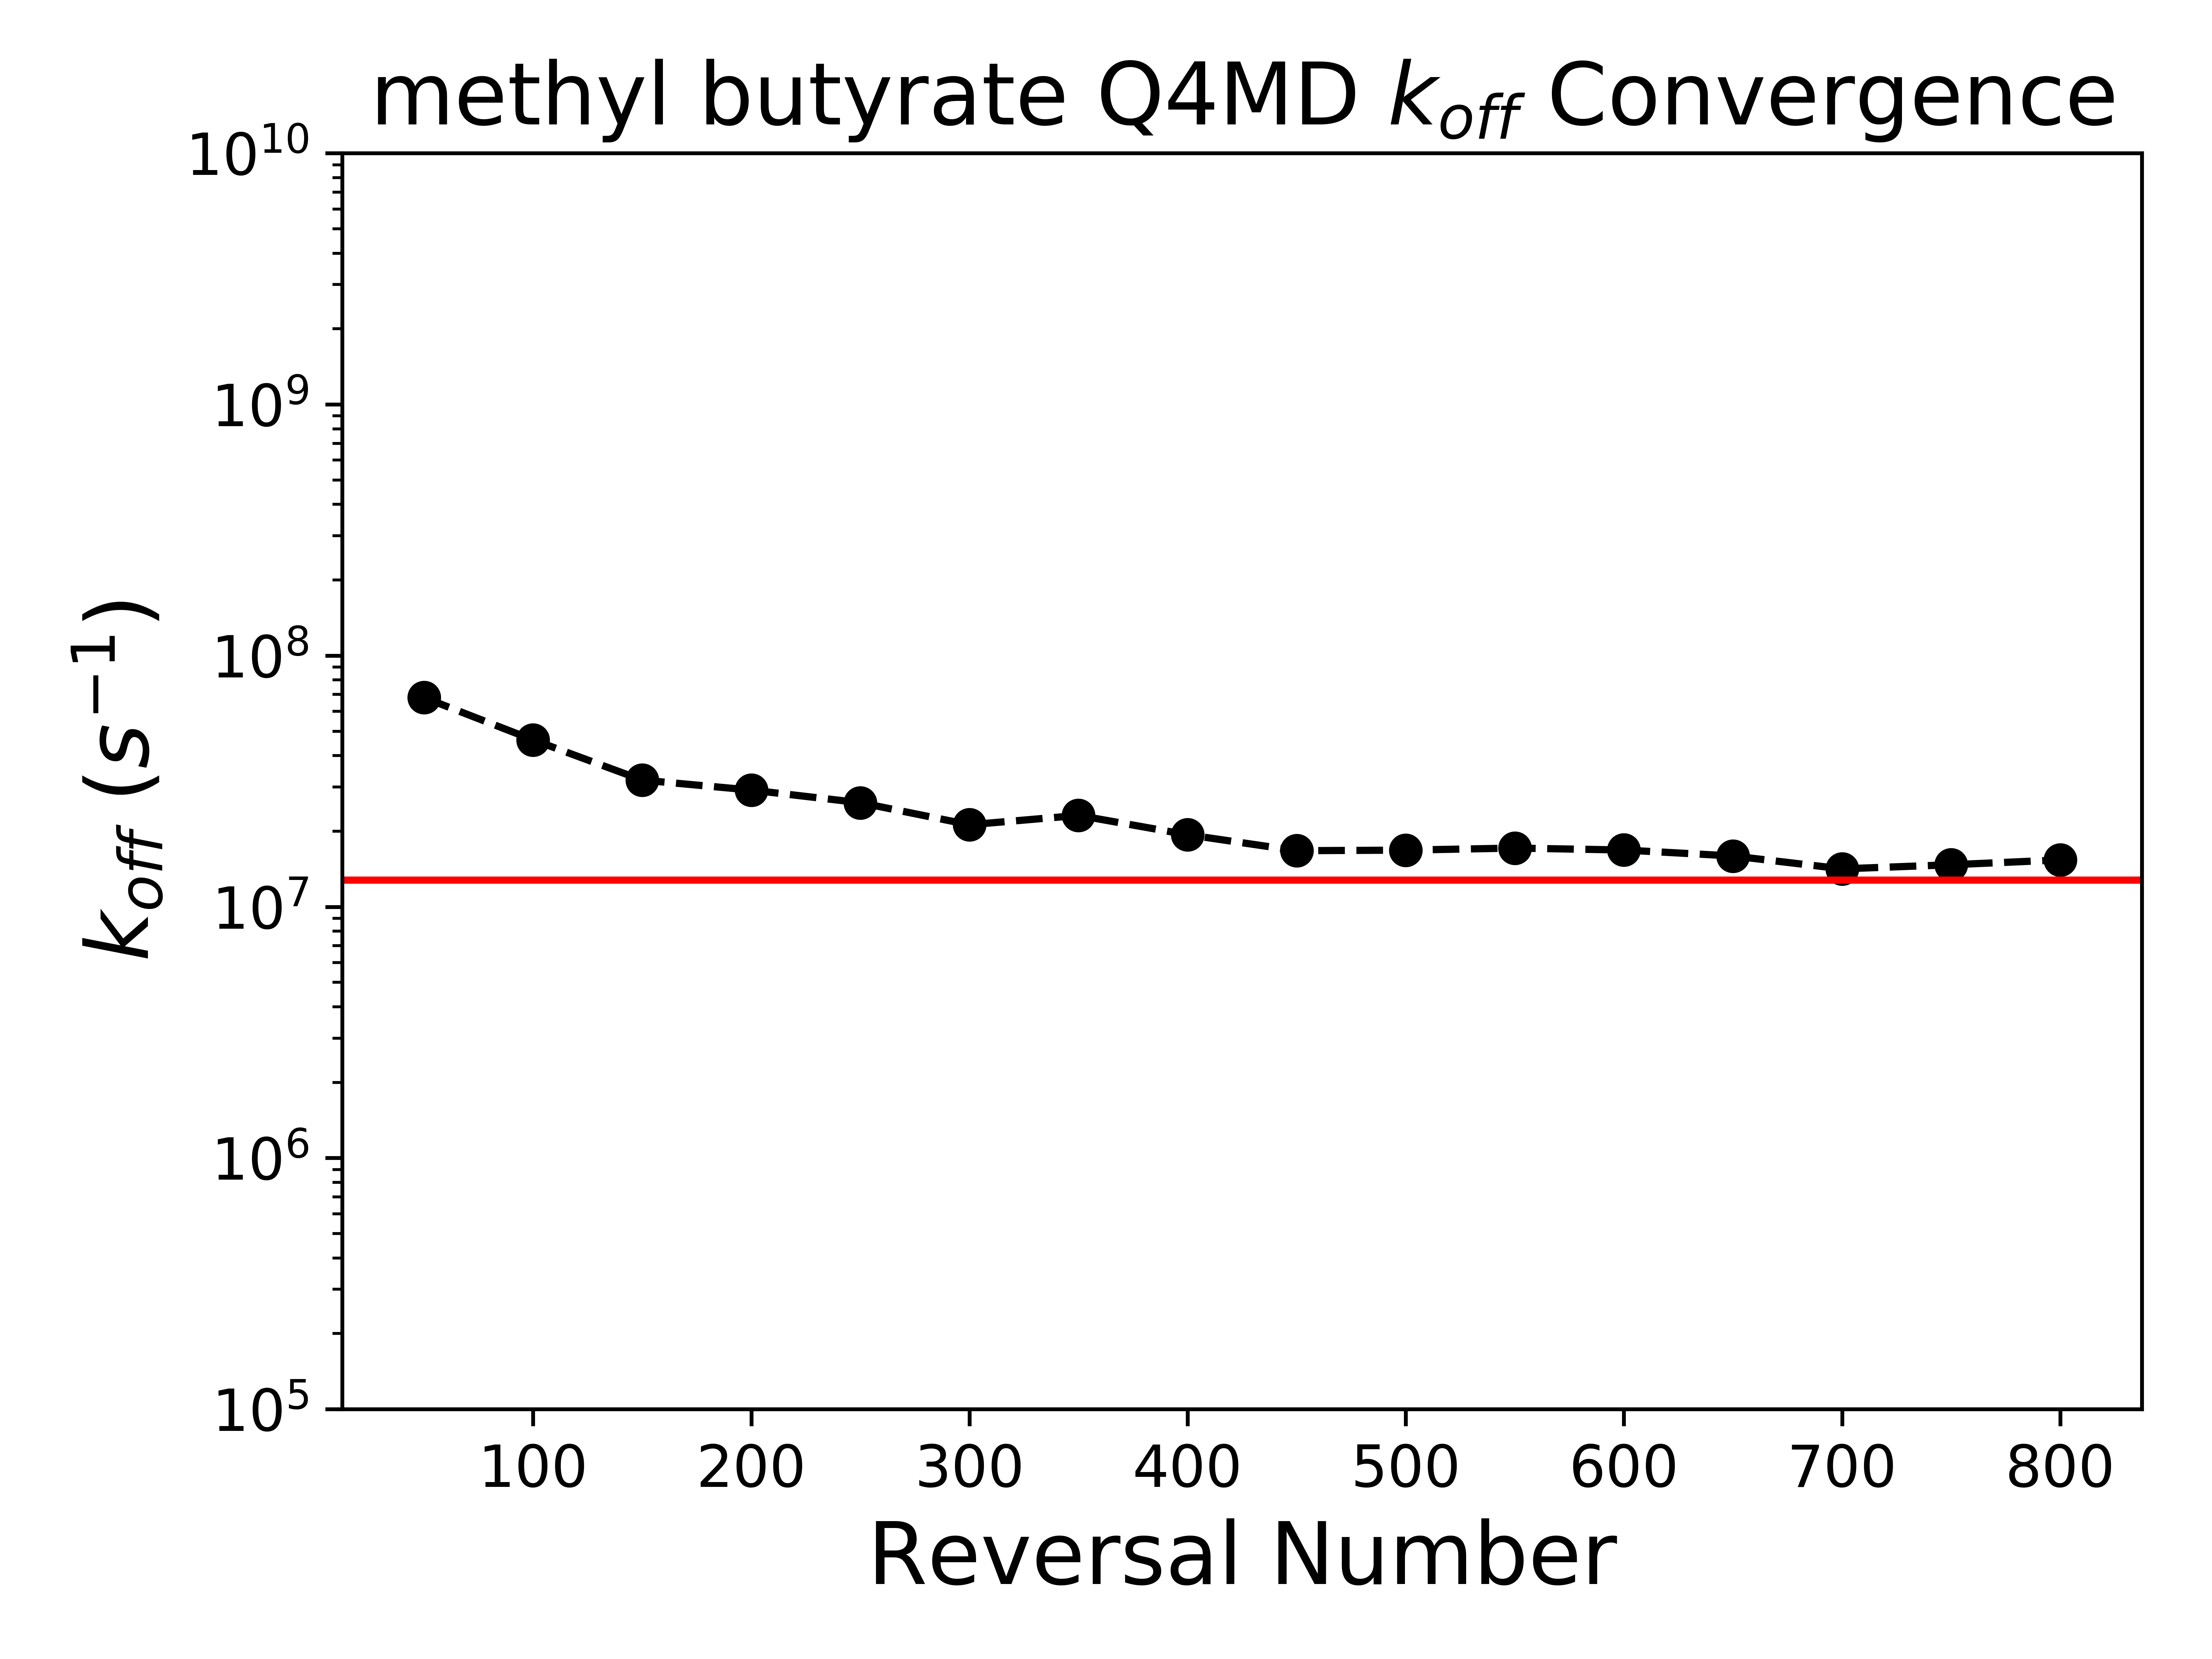
\includegraphics[width=\linewidth]{high_res_images/q4md_rate_conv_images/methylbutyrate_q4md_off_conv.png}
	\end{subfigure}
	\begin{subfigure}{0.3\linewidth}
		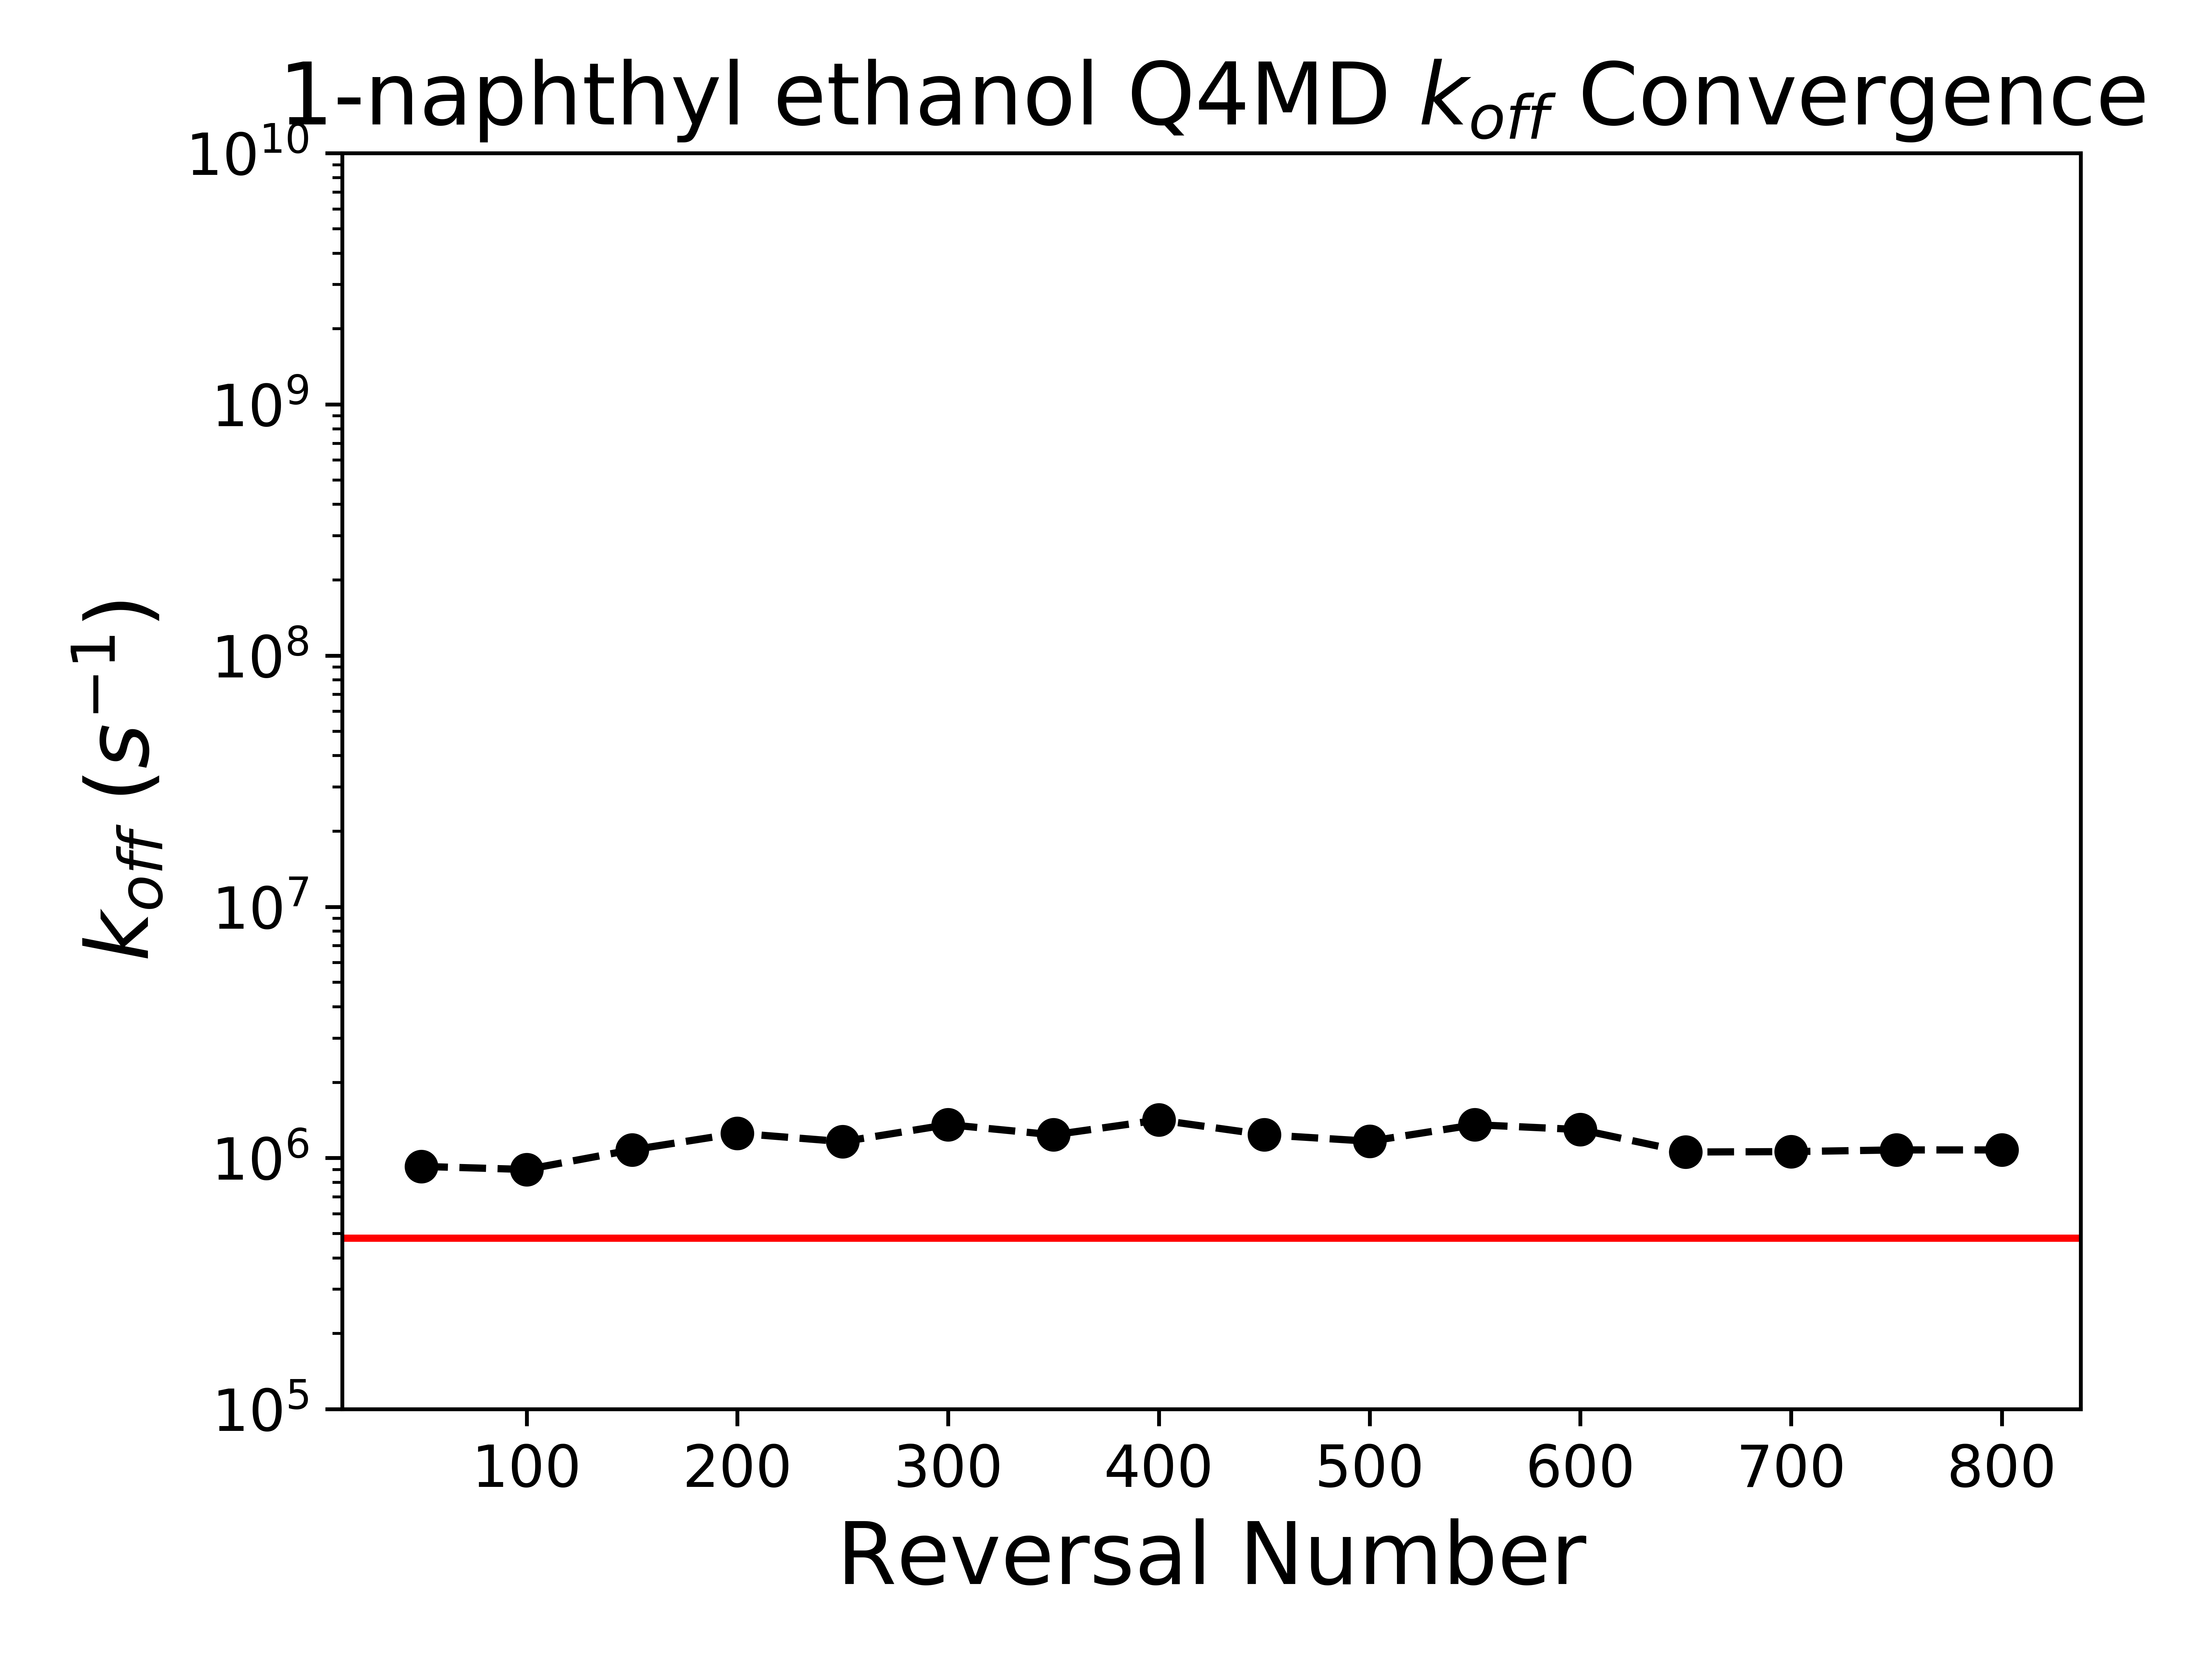
\includegraphics[width=\linewidth]{high_res_images/q4md_rate_conv_images/1-naphthylethanol_q4md_off_conv.png}
	\end{subfigure}
	\begin{subfigure}{0.3\linewidth}
		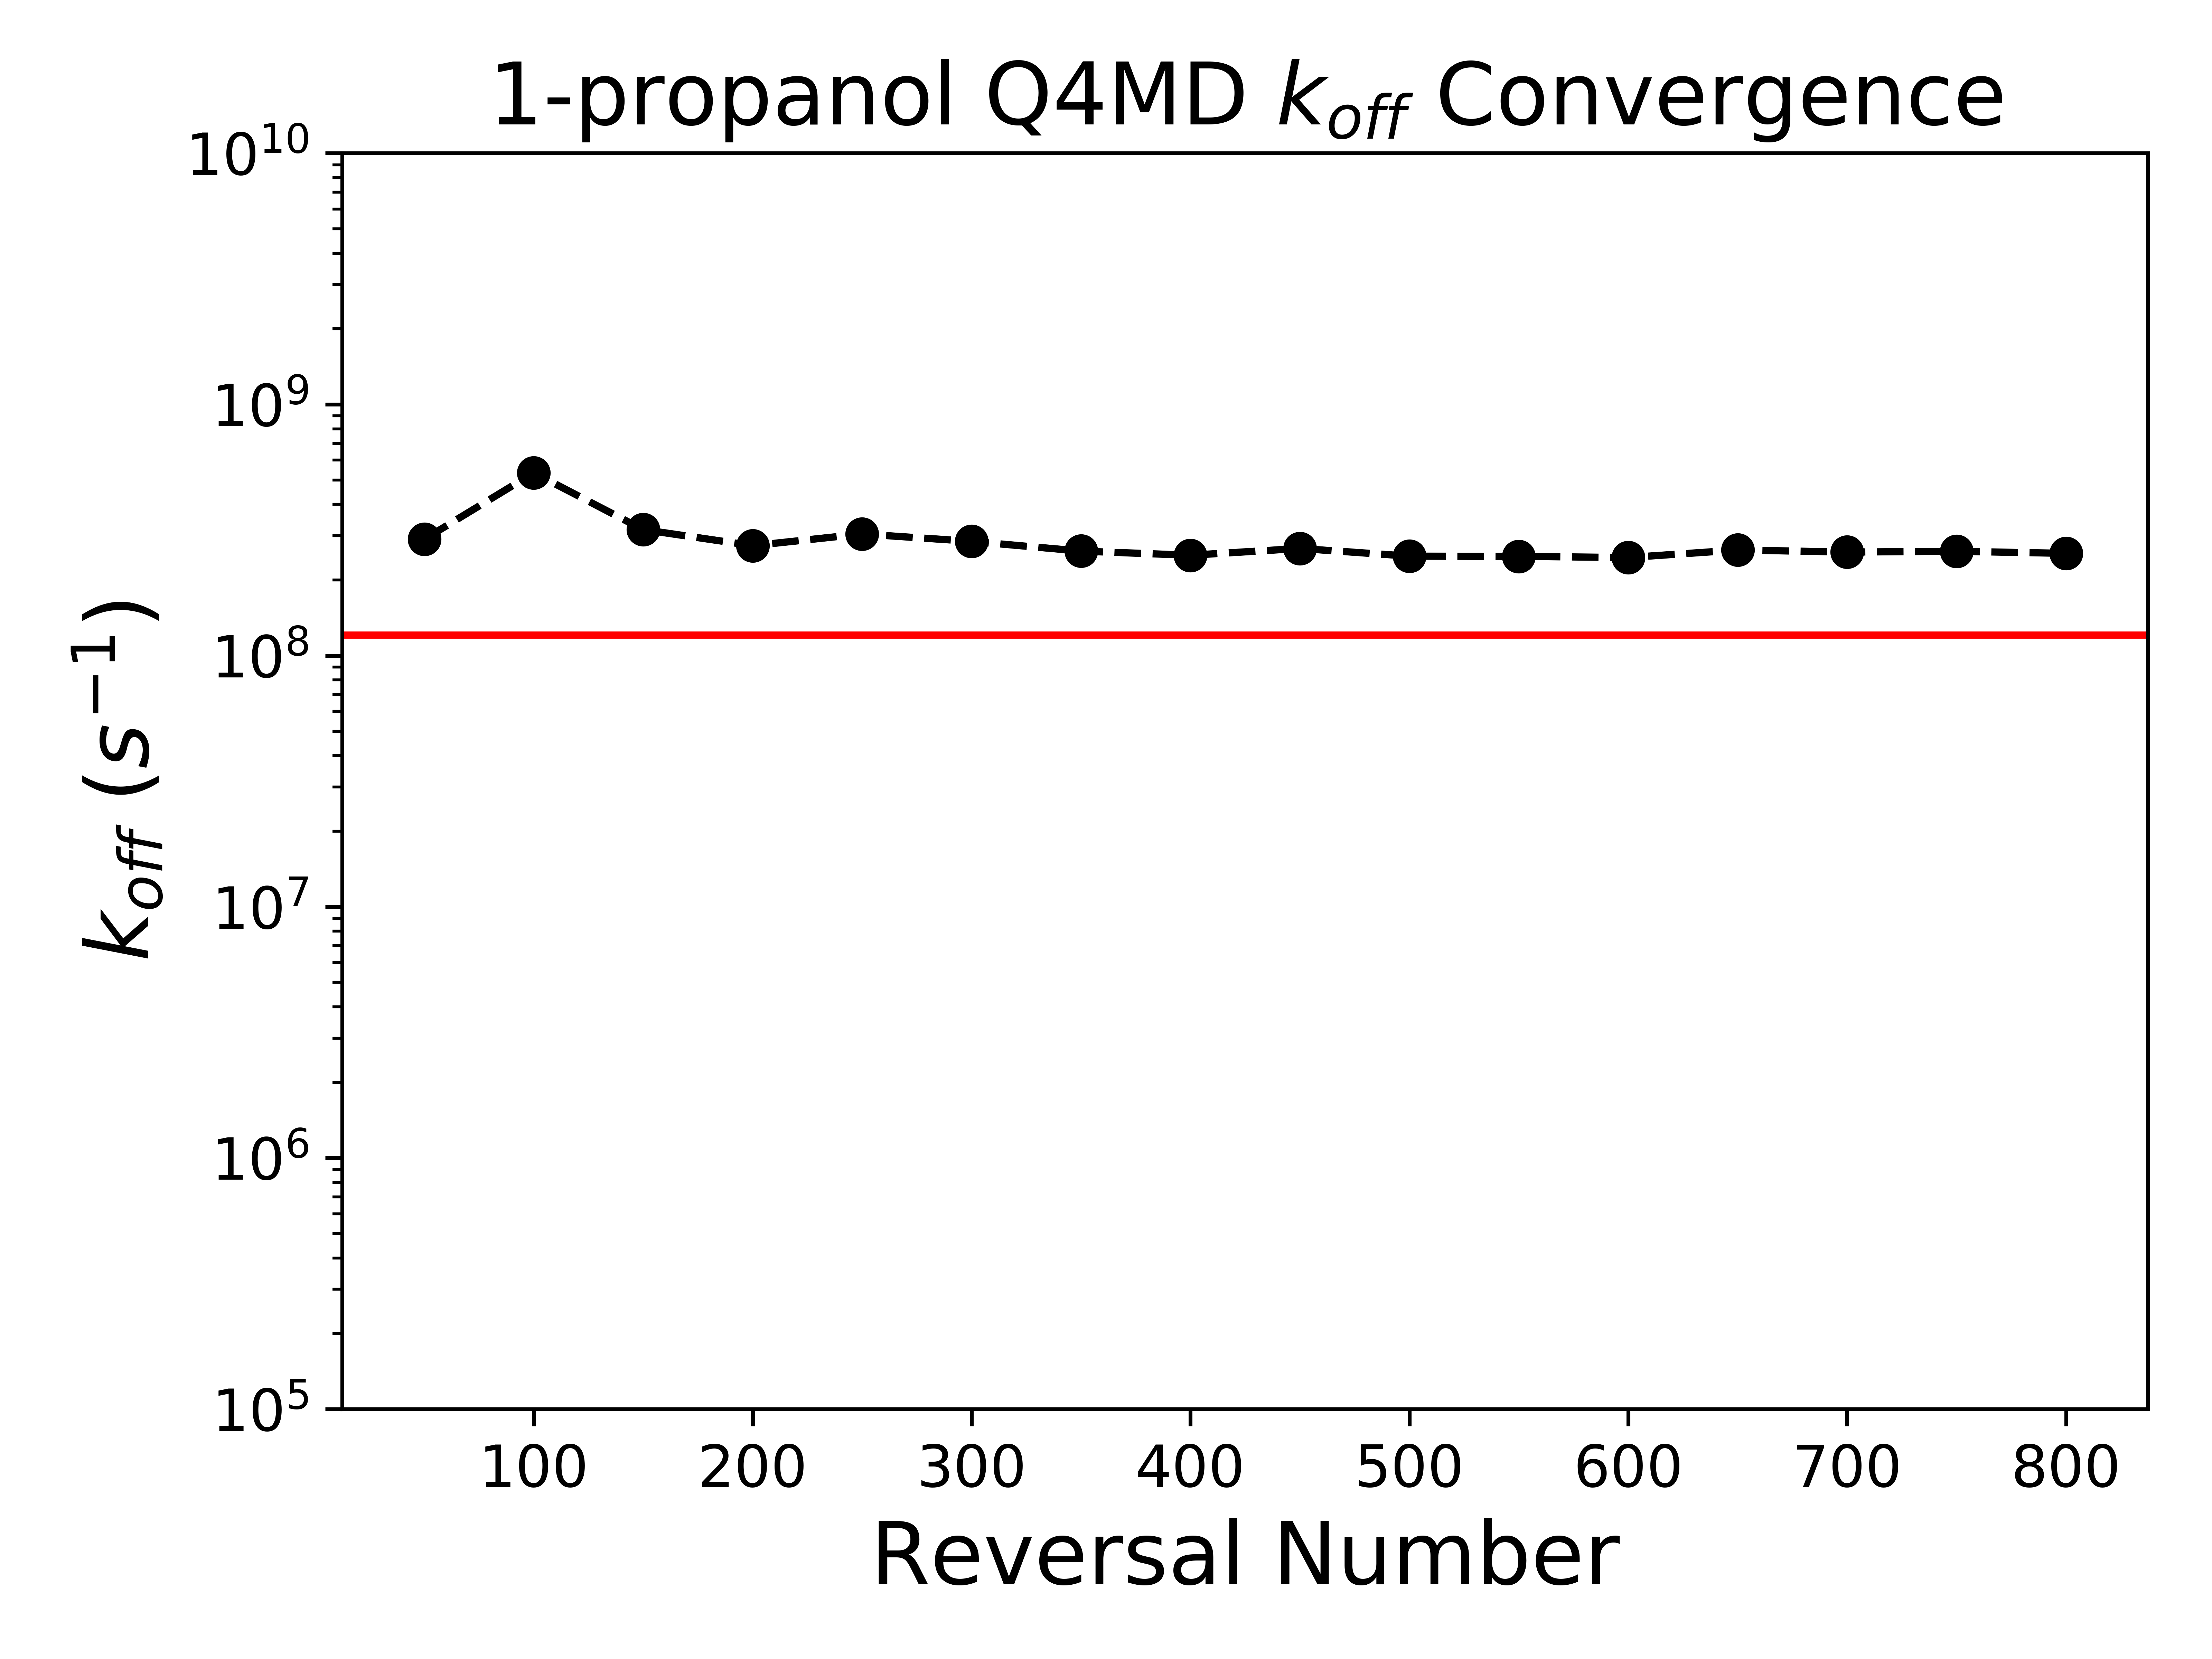
\includegraphics[width=\linewidth]{high_res_images/q4md_rate_conv_images/1-propanol_q4md_off_conv.png}
	\end{subfigure}
	\begin{subfigure}{0.3\linewidth}
		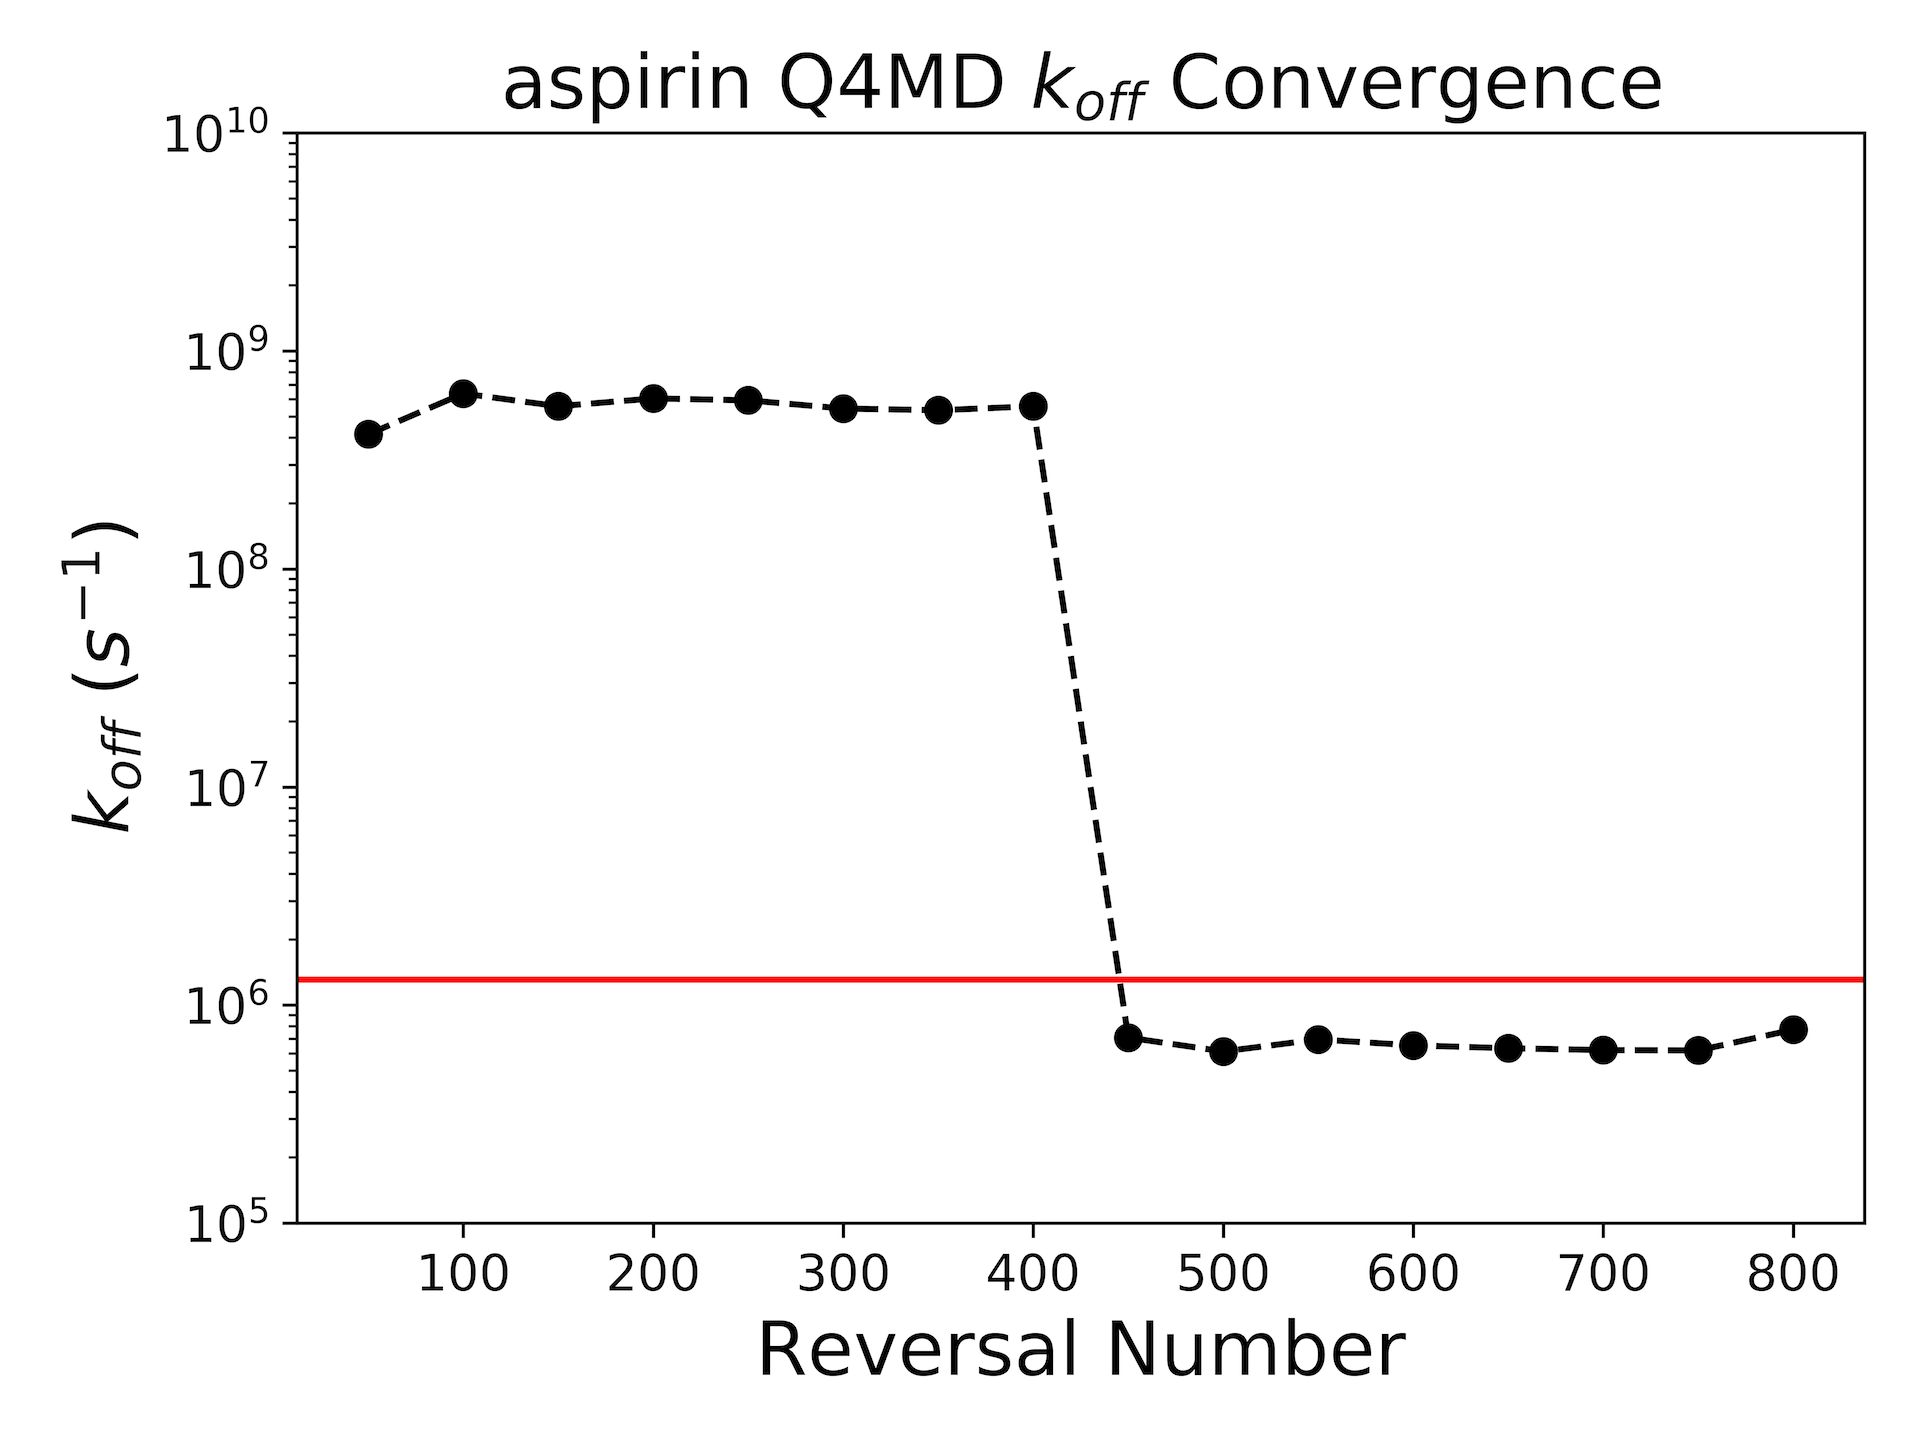
\includegraphics[width=\linewidth]{high_res_images/q4md_rate_conv_images/aspirin_q4md_off_conv.png}
	\end{subfigure}
	\caption{Convergence of off rates as a function of the number of reversals included using the Q4MD forcefield}
\end{figure}

\par Convergence of the rate constant is a highly complicated quantity dependent 
on the transition probabilities as well as the incubation times obtained from 
each milestone. Therefore, a more detailed analysis of the convergence of 
these quantities on a per milestone level can provide further insight into the 
overall convergence of a rate calculation within SEEKR. Fig.~\ref{fig:aspirin_conv_fig}a,b shows the convergence
of \kon and \koff, respectively, as a function of the number of reversals
launched for the representative system of Q4MD \bcd with aspirin. Reversal number is directly related to the length of
equilibrium sampling, the current bottleneck of a SEEKR
calculation.
While both values appear to converge in fewer than the maximum
number of reversals, the dramatic change in \koff after
reversal number 400 is of note. Further analysis of the
per-milestone transition counts (Fig.~\ref{fig:aspirin_conv_fig}c) and
incubation times (Fig.~\ref{fig:aspirin_conv_fig}d) revealed
that this change in \koff was due to poor initial sampling of
the -1.5 \AA milestone, which once sampled decreased the overall \koff. 

\begin{figure}
	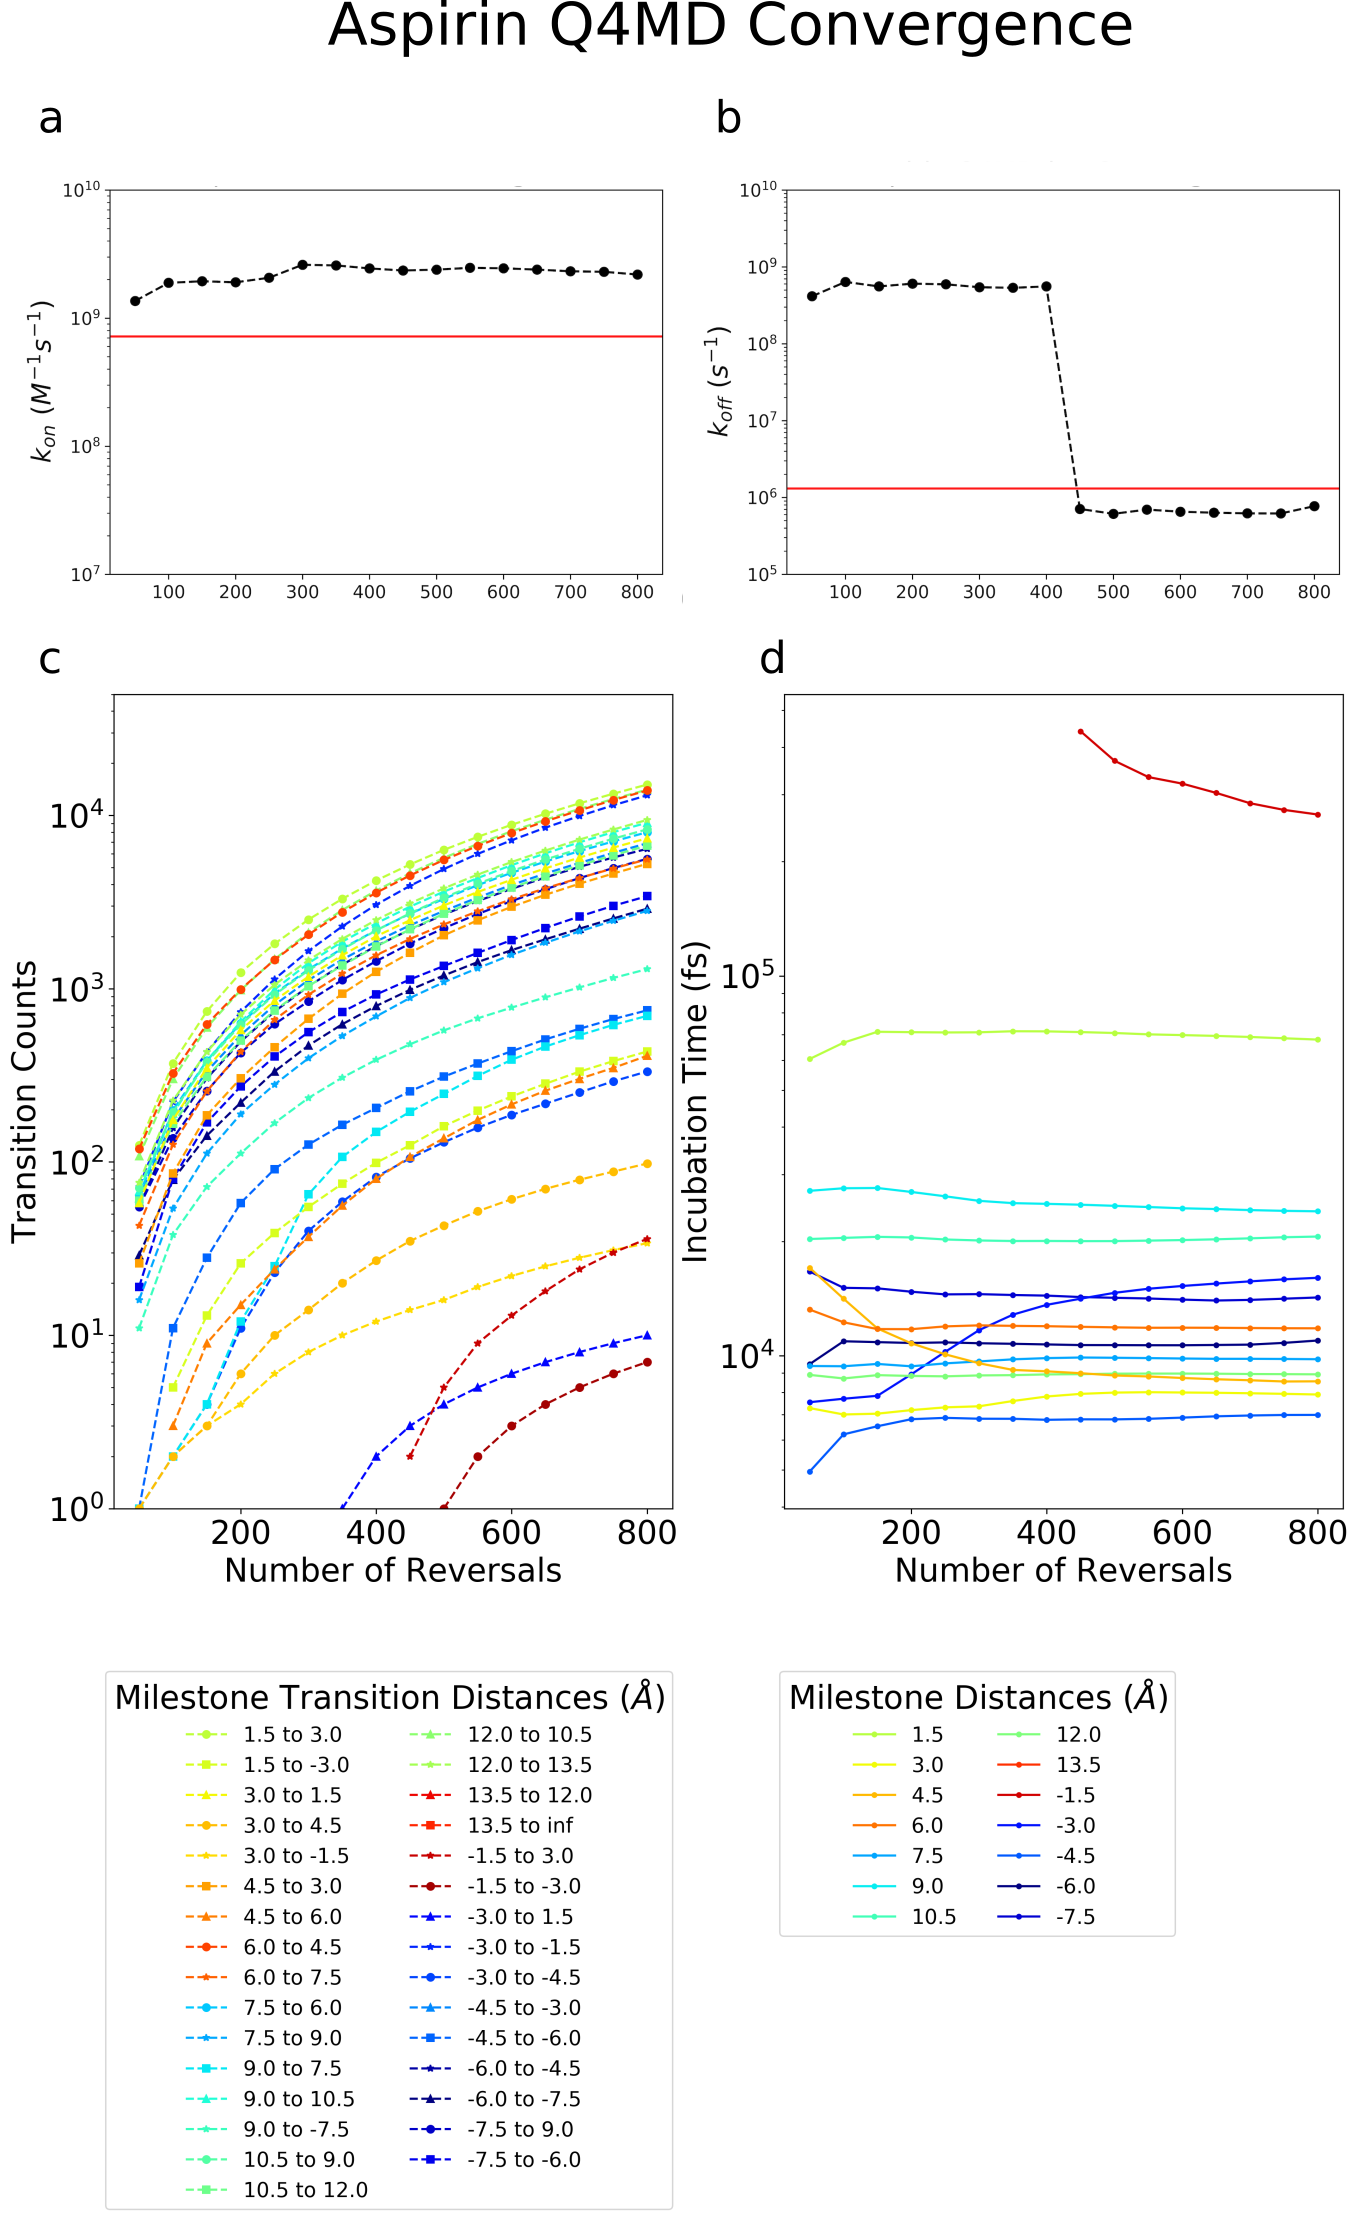
\includegraphics{images/aspirin_conv_comb.png}

	\caption{Convergence analysis for a representative ligand,  aspirin, and \bcd with the Q4MD forcefield. Convergence of a) \kon, b) \koff,  c) transition counts, and d) incubation times for each milestone are plotted as a function of the number of reversals launched.  Reversal number is directly related to the length of equilibrium sampling, as reversals were launched at 2 ns intervals from the equilibrium trajectory.}
	\label{fig:aspirin_conv_fig}
\end{figure}

This was only observed for the aspirin ligand, one of the bulkiest ligands, where it was extremely unlikely to observe transitions outward from the primary face due to steric effects. 
Evaluation of these convergence properties on a 
per milestone basis is a valuable diagnostic tool; identifying which 
milestones contribute most to the mean first passage time (and therefore \kon 
and \koff) and milestones where the ligand spends only a short time, providing 
detailed molecular insight into the binding and unbinding processes.
Furthermore, this analysis is also useful during the simulation process, 
as the convergence of each milestone can be assessed ``on the fly'' and individual simulations 
can be terminated or extended accordingly for each milestone.



%\subsubsection*{Milestoning Model}
\par We also explore the sensitivity of the calculated rate constants to the milestoning model construction. In particular, the appropriate 
spacing of milestones is critical for the calculation. Milestones must not be 
spaced so close such that the velocity of the system cannot decorrelate between 
transitions \cite{Vanden-Eijnden2008,West2007}. This assumption is typically 
valid for molecular dynamics simulations, as velocities typically decorrelate on 
the subpicosecond timescale \cite{Vanden-Eijnden2008}. However, if milestones are 
spaced far apart, transitions will require much longer simulations and 
milestioning sampling efficiency is lost.

For our systems, the incubation times of all milestones are on the order 
of multiple picoseconds or greater, which 
is longer than the sub-picosecond timescale typically necessary for decorrelation\cite{Vanden-Eijnden2008}.
When the milestone spacing was doubled to 3~\AA, simulation efficiency was 
dramatically reduced, such that few to no transitions between milestones were 
observed, precluding the calculation of rate constants. These observations suggest 
that the 1.5~\AA spacing used in our simulations was appropriate for the 
calculation of the desired kinetic parameters.

\par Our milestoning model differentiates the two faces 
of the cyclodextrin ring and therefore defines two bound states, corresponding 
to each face. Investigation into the effect of this on the resulting rate 
constants revealed that it had only minimal effects. When the two bound states 
were combined into a single milestone, only small changes to the rate were 
observed, within the error of both calculations. Furthermore, when the the two 
faces were not differentiated with unique milestones, minimal change in the 
calculated rate constants was observed. 

%\par We calculated the rates using both 
%milestoning models for the Q4MD system, where the calculated rate values are 
%smaller than the GAFF system and therefore changes in the value would be more 
%influential on the overall result.

%\par The calculated off rate values of all ligands were within the calculated 
%errors from both models. The only calculated on rate value that did not fall 
%within the error was aspirin, where the on rate increased from  
%$(2.19 \pm 0.12)\times 10^9$ $M^{-1}s^{-1}$ to $(2.90 \pm 0.14)\times 10^9$ $M^{-1}s^{-1}$.
%The minimal effect of these changes in the milestoning model on the calculated 
%rates is likely due to the extensive sampling achieved on both faces.

\par It is also important to note that our milestoning model did not explicitly 
resolve the ligand orientation in any way, and therefore any ligand orientational 
sampling was achieved entirely through simulation. This resulted in some ligand 
orientations being unsampled in the deepest milestones where the orientation was 
sterically restricted to the starting conformation on that milestone. While this 
is a limitation that will be addressed in future developments of SEEKR, it also 
highlights that a relatively simplistic model was able effectively calculate 
kinetic parameters with good agreement to experimental values.

\par The simplicity of this model has many advantages. The bound state is 
defined naturally as the innermost milestone and all other milestones can be 
defined at the same time, including what defines the unbound state. The long 
timescale MD employed a more empirical definition of the bound state where the 
ligand was only considered bound when the COM of the ligand was within 7.5~\AA 
of the COM of the $\beta$-cyclodextrin for at least 1.0~ns. Similarly the ligand 
was considered unbound when it left this 7.5~\AA bound state for at least 1.0~ns.
With the SEEKR approach, minimal prior knowledge of the system is required, as 
binding and unbinding are determined only from the milestone surfaces. No time 
cutoff is required, as short excursions that do not result in full binding and 
unbinding events are captured naturally in the milestoning model. The simplicity of SEEKR milestoning calculation setup, in conjunction with
the ability to monitor convergence for each milestone and terminate
simulations accordingly, makes this approach well-suited for
calculations with multiple ligands as would be necessary in a drug
discovery setting.